%  LaTeX support: latex@mdpi.com 
%  In case you need support, please attach all files that are necessary for compiling as well as the log file, and specify the details of your LaTeX setup (which operating system and LaTeX version / tools you are using).

%=================================================================
\documentclass[energies,article,submit,moreauthors,pdftex]{Definitions/mdpi} 

\usepackage{graphicx}
% \usepackage{subfig}
\usepackage{subcaption}
\usepackage{algorithm2e}
\usepackage{listings}

% \usepackage{}
% If you would like to post an early version of this manuscript as a preprint, you may use preprint as the journal and change 'submit' to 'accept'. The document class line would be, e.g., \documentclass[preprints,article,accept,moreauthors,pdftex]{mdpi}. This is especially recommended for submission to arXiv, where line numbers should be removed before posting. For preprints.org, the editorial staff will make this change immediately prior to posting.



%---------
% article
%---------
% The default type of manuscript is "article", but can be replaced by: 
% abstract, addendum, article, benchmark, book, bookreview, briefreport, casereport, changes, comment, commentary, communication, conceptpaper, conferenceproceedings, correction, conferencereport, expressionofconcern, extendedabstract, meetingreport, creative, datadescriptor, discussion, editorial, essay, erratum, hypothesis, interestingimages, letter, meetingreport, newbookreceived, obituary, opinion, projectreport, reply, retraction, review, perspective, protocol, shortnote, supfile, technicalnote, viewpoint
% supfile = supplementary materials

%----------
% submit
%----------
% The class option "submit" will be changed to "accept" by the Editorial Office when the paper is accepted. This will only make changes to the frontpage (e.g., the logo of the journal will get visible), the headings, and the copyright information. Also, line numbering will be removed. Journal info and pagination for accepted papers will also be assigned by the Editorial Office.

%------------------
% moreauthors
%------------------
% If there is only one author the class option oneauthor should be used. Otherwise use the class option moreauthors.

%---------
% pdftex
%---------
% The option pdftex is for use with pdfLaTeX. If eps figures are used, remove the option pdftex and use LaTeX and dvi2pdf.

%=================================================================
\firstpage{1} 
\makeatletter 
\setcounter{page}{\@firstpage} 
\makeatother
\pubvolume{xx}
\issuenum{1}
\articlenumber{5}
\pubyear{2020}
\copyrightyear{2020}
%\externaleditor{Academic Editor: name}
\history{Received: date; Accepted: date; Published: date}
%\updates{yes} % If there is an update available, un-comment this line

%% MDPI internal command: uncomment if new journal that already uses continuous page numbers 
%\continuouspages{yes}

%=================================================================
% Add packages and commands here. The following packages are loaded in our class file: fontenc, calc, indentfirst, fancyhdr, graphicx, lastpage, ifthen, lineno, float, amsmath, setspace, enumitem, mathpazo, booktabs, titlesec, etoolbox, amsthm, hyphenat, natbib, hyperref, footmisc, geometry, caption, url, mdframed, tabto, soul, multirow, microtype, tikz

%=================================================================
%% Please use the following mathematics environments: Theorem, Lemma, Corollary, Proposition, Characterization, Property, Problem, Example, ExamplesandDefinitions, Hypothesis, Remark, Definition, Notation, Assumption
%% For proofs, please use the proof environment (the amsthm package is loaded by the MDPI class).

%===============================================================
%                           TITLE & AUTHORS
%===============================================================
% Full title of the paper (Capitalized)
\Title{Impact of the COVID-19 Lockdown on Electricity System in Great Britain: a Study on Energy Demand, Generation, Pricing and Grid Stability}

% Author Orchid ID: enter ID or remove command
\newcommand{\orcidauthorA}{0000-0001-7596-0944} % Add \orcidA{} behind the author's name
\newcommand{\orcidauthorB}{0000-0002-3494-0469} % Add \orcidB{} behind the author's name

% Authors, for the paper (add full first names)
\Author{Desen Kirli $^{1,*,}$\orcidA{}, Maximilian Parzen $^{1}$ and Aristides Kiprakis $^{1,}$\orcidB{}}

% Authors, for metadata in PDF
\AuthorNames{Firstname Lastname, Firstname Lastname and Firstname Lastname}

% Affiliations / Addresses (Add [1] after \address if there is only one affiliation.)
\address{%
$^{1}$ \quad Institute for Energy Systems, School of Engineering, University of Edinburgh\\}
% $^{2}$ \quad Affiliation 2; e-mail@e-mail.com}

% Contact information of the corresponding author
\corres{Correspondence: desen.kirli@ed.ac.uk}
%; Tel.: (optional; include country code; if there are multiple corresponding authors, add author initials) +xx-xxxx-xxx-xxxx (F.L.)

% Current address and/or shared authorship
% \firstnote{Current address: Affiliation 3} 
% \secondnote{These authors contributed equally to this work.}
% The commands \thirdnote{} till \eighthnote{} are available for further notes


%===============================================================
%                           ABSTRACT & KEYWORDS
%===============================================================

% Abstract (Do not insert blank lines, i.e. \\) 
\abstract{
%Electricity is both a vital service and necessity at all times yet even more critical during a pandemic. 
The outbreak of SARS-COV-2 disease 2019 (COVID-19) abruptly changed the patterns in electricity consumption, challenging the system operations of forecasting and balancing the supply and demand. This is due to the mitigation measures that include lockdown and Work from Home (WFH) which decreased the aggregated demand and altered its profile remarkably. In this paper, we characterise these changes with various quantitative markers and compare it with pre-COVID-19 business-as-usual data using the case study of Great Britain. The ripple effects on the generation portfolio, system frequency, accuracy of forecasting and imbalance pricing are also analysed. An energy data extraction and pre-processing pipeline that can be used in a variety of similar studies is also presented.}
%  Electricity is both a vital service and necessity at all times yet even more critical during a pandemic. The ongoing outbreak of coronavirus disease 2019 (COVID-19) has abruptly changed the patterns in electricity consumption, challenging the system operators who forecast and match the electricity supply and demand. This is due to the mitigation measures that include self-isolation, lockdown and working remotely which decreased the aggregated demand and altered its profile remarkably. In this paper, we characterise the changes in the demand profile with various quantitative markers and compare it with pre-COVID-19 business-as-usual data using the case study of Great Britain. The impact on the generation portfolio and pricing is also analysed using the value factor method. We present a timeline of the pandemic mitigation actions taken and the corresponding changes in the demand profile and energy portfolio. The volume of demand-side response services is also analysed against the historic data that shows (?) an increase. ?maybe include frequency services and comment on it as a grid stability measure? + the main conclusions or interpretations - once we have them :)

% A single paragraph of about 200 words maximum. For research articles, abstracts should give a pertinent overview of the work. We strongly encourage authors to use the following style of structured abstracts, but without headings: (1) Background: Place the question addressed in a broad context and highlight the purpose of the study; (2) Methods: Describe briefly the main methods or treatments applied; (3) Results: Summarize the article's main findings; and (4) Conclusion: Indicate the main conclusions or interpretations. The abstract should be an objective representation of the article, it must not contain results which are not presented and substantiated in the main text and should not exaggerate the main conclusions

% Keywords (list 3 to 10 pertinent keywords specific to the article, yet reasonably common within the subject discipline.
\keyword{electricity system, COVID-19, electricity demand, demand-side response}


%===============================================================
%                           MAIN TEXT
%===============================================================

\begin{document}
% \tableofcontents
%===============================================================
%                           INTRO
%===============================================================
% \textbf{***ENERGIES -SPECIAL ISSUES ON COVID-19***}

% (1) \textbf{Special Issue COVID-19 Pandemics: Energy, Economic, Environmental, Social, Policy and Health Impacts}
% \url{https://www.mdpi.com/journal/energies/special\_issues/covid\_energy\_economic\_environmental\_social\_policy\_health}


% (2) \textbf{Special Issue Coronavirus Crisis, Energy Markets and Policies and Their Macro-Financial Implications}
% \url{https://www.mdpi.com/journal/energies/special_issues/Coronavirus_Crisis_Energy_Markets_Policies_Their_Macro_Financial_Implications}




% \textcolor{blue}{\textbf{***SIMILAR ANALYSIS - COVID-19 \& Elect Demand***}}

% (1) \textbf{UKERC Report: Electricity demand during week one of COVID-19 lockdown}
% \url{http://www.ukerc.ac.uk/news/covid-lockdown-electricity-demand.html}

% (2) \textbf{EPRI Report: COVID-19 Bulk System Impacts Demand Impacts and Operational and Control Centers}
% \url{http://mydocs.epri.com/docs/public/covid19/3002018602R2.pdf}

% (3) \textbf{Aurora Report: Impact of Coronavirus on European energy markets}
% \url{https://www.auroraer.com/wp-content/uploads/2020/04/Aurora-COVID-19-weekly-impact-tracker-090420-.pdf}

% (4) \textbf{HIGHEST SYSTEM PRICE SINCE}
% \url{https://www.elexon.co.uk/article/elexon-insight-highest-system-price-in-19-years/}

% (5) \textbf{The 'lockdown effect' on TV viewing habits and the electricity grid}
% \url{https://www.nationalgrideso.com/news/lockdown-effect-tv-viewing-habits-and-electricity-grid}


% (6) \textbf{NEW UN REPORT ON THE COVID-19 IMPACT ON THE SDG - includes low-carbon generation goals.}
% \url{bit.ly/2WZI3I4}


% \url{https://www.elexon.co.uk/article/coronavirus-temporary-derogations-to-improve-settlement-accuracy/}

\section{Introduction}
%%%%%%%%%%%%%%%%%%%%%%%%%%%%%%%%%%%%%%%%%%%
% 1. Provide background information and set the context.
% 2. Introduce the specific topic of your research and explain why it is important.
% 3. Mention past attempts to solve the research problem or to answer the research question.
% 4. Conclude the Introduction by mentioning the specific objectives of your research.
%%%%%%%%%%%%%%%%%%%%%%%%%%%%%%%%%%%%%%%%%%%%%%%%%%%%%%%%%
% No.1
The outbreak of coronavirus disease 2019 (COVID-19) lead in UK on 23rd of March to a lockdown. Prime Minister Boris Johnson addressed on this day to the nation that Britons should only go outside to buy food, to exercise, or to go to work if home office was not possible. Citizens would face police fines for failing the new measures \cite{BritishForeignPolicyGroup2020COVID-19Timeline}. 
% No.2
These drastic measures lead to disruptive change in the demand and influenced the wider energy sector. The analysis of this high impact and low probability event is important, as with the insights one could possibly anticipate any adverse effects on the electricity sector in future pandemic situations. 
% No.3
%Small literature study of attempts to analyse the impacts on the electricity sector.(Share love, mention many papers and summarise how our work extend previous work)
% No.4
As result this study seeks to quantify the changes in demand, generation, grid stability and market prices.

% Electricity is a vital service at all times. In the UK, the utilities sector was identified as critical for the continuation of essential public services by the government. As it is essential to meet the heat and lighting demand for 
% homes, businesses to function and for the NHS to care for the sick.

%The outbreak of coronavirus disease 2019 (COVID-19) decoupled the electricity demand from its fundamental prediction elements which are namely the weather conditions and periodicity or time. In other words, the electricity demand forecasting methods mainly rely on the correlation with weather data (temperature in specific) and recurrence or periodical habits (e.g. evening demand peak after 5pm or expected increase on the Christmas Eve). [!ref]

%...

 %In response to the increase in the number of COVID-19 cases, the UK government announced new rules that included lockdown, closure of businesses and remote working to mitigate the spread of the coronavirus on 23rd March 2020. The massive shift to home and remote working and closure of office spaces, schools, factories and similar resulted in a different electricity consumption profile.




%===============================================================
%                           METHODS
%===============================================================
 %CHANGED
\section{Methodology\label{section:Methodology}}
In order to analyse the impact of the COVID-19 lockdown on the electricity market, a systematic approach is used which involved creating an efficient pipeline to extract the target data, pre-process, analyse and visualise. In this section, the methodology used in the pipeline is explained. The instructions for future use are detailed using a flow diagram. The actual Python code employed can be accessed at the GitHub repository\footnote{https://github.com/desenk/Electricity-Data-Pipeline} \cite{KirliElectricityPipeline} and in Appendix \ref{section:PipelineCode}. Both .py and .ipynb formats are made available on \cite{KirliElectricityPipeline}.

%What the code does%
\subsection{Function of the Data Pipeline Code}
As this study involves a comparative analysis, various actions, such as cleaning the data and calculating the percentage differences, had to be repeated for different data sets like frequency and demand. In order to minimise the time spent from the import of the data to the analysis and visualisation stages, a data pipeline on Python is programmed to fetch the data directly using the application programming interface (API) of the provider - see \cite{KirliElectricityPipeline} and Appendix \ref{section:PipelineCode}. This process is also commonly referred to as scripting, extracting and scraping the data. This pipeline is used for analysing the system frequency, demand, generation and other types of data and all results are presented in Section \ref{section:Results}.  It performs the following steps listed below. 


% \begin{enumerate}
%     \item Import the data from the source webpage using the API user key
%     \item Identify the keywords and group the data
%     \item Create weekly data frames (according to the Monday-to-Sunday convention (i.e. ISO 8601))
%     \item Check for zeros ,invalid or duplicate data
%     \item Label and discard the columns that are not of interest
%     \item Adjust the date and time format (e.g. change from half-hourly settlement period convention (where 01:00 is denoted by 2) to time)
%     \item Save the adjusted data in CSV format with an automated title  (\texttt{$DataLabel$\_Week\_starting\_$StartDate$.csv})
%     \item Calculation of statistical and other quantitative descriptors such as mean, peak-to-mean ratio, etc.
%     \item Comparative visualisation of the data
% \end{enumerate}


\begin{algorithm}[H]
\SetAlgoLined
\KwResult{Extraction, pre-processing, analysis and visualisation of the GB electricity data}
\begin{enumerate}
    \item Import the data from the source webpage using the API user key
    \item Identify the keywords and group the data
    \item Create weekly data frames (according to the Monday-to-Sunday convention (i.e. ISO 8601))
    \item Check for zeros, invalid or duplicate data
    \item Label the columns and discard any that are not of interest
    \item Adjust the date and time format (e.g. change from half-hourly settlement period convention (where 01:00 is denoted by 2) to time)
    \item Save the pre-processed data in the CSV format with an automated title  (\texttt{$DataLabel$\_Week\_starting\_$StartDate$.csv})
    \item Calculation of statistical and other quantitative descriptors such as mean, peak-to-mean ratio, etc.
    \item Comparative visualisation of the data
\end{enumerate}
 
 \caption{The Electricity Data Pipeline}
\end{algorithm}

%How can my code can be used for other projects%
\subsection{Using the Data Pipeline for other research}
In most of our analysis cases, the data source is the Balancing Mechanism Reporting Service (BMRS) \cite{Elexon2019BMRSArchitecture}. The website \cite{ElectricityBMRS} provides open-source data that is used for the balancing and settling the GB electricity system.

The data provided (e.g. system  demand, frequency, generation by fuel type, etc.) is used for reaching trading decisions and analysing the dynamics of market volumes and pricing. Hence, we believe that this pipeline may be useful for both academic and industrial researchers who are interested in electricity market dynamics, regulation, trading and forecasting as it enables easy data extraction, pre-processing and visualisation. The flowchart in Figure \ref{fig:pipeline_flowchart}, displays the steps required to replicate the results.


\begin{figure}[H]
\centering
\hspace{-25pt}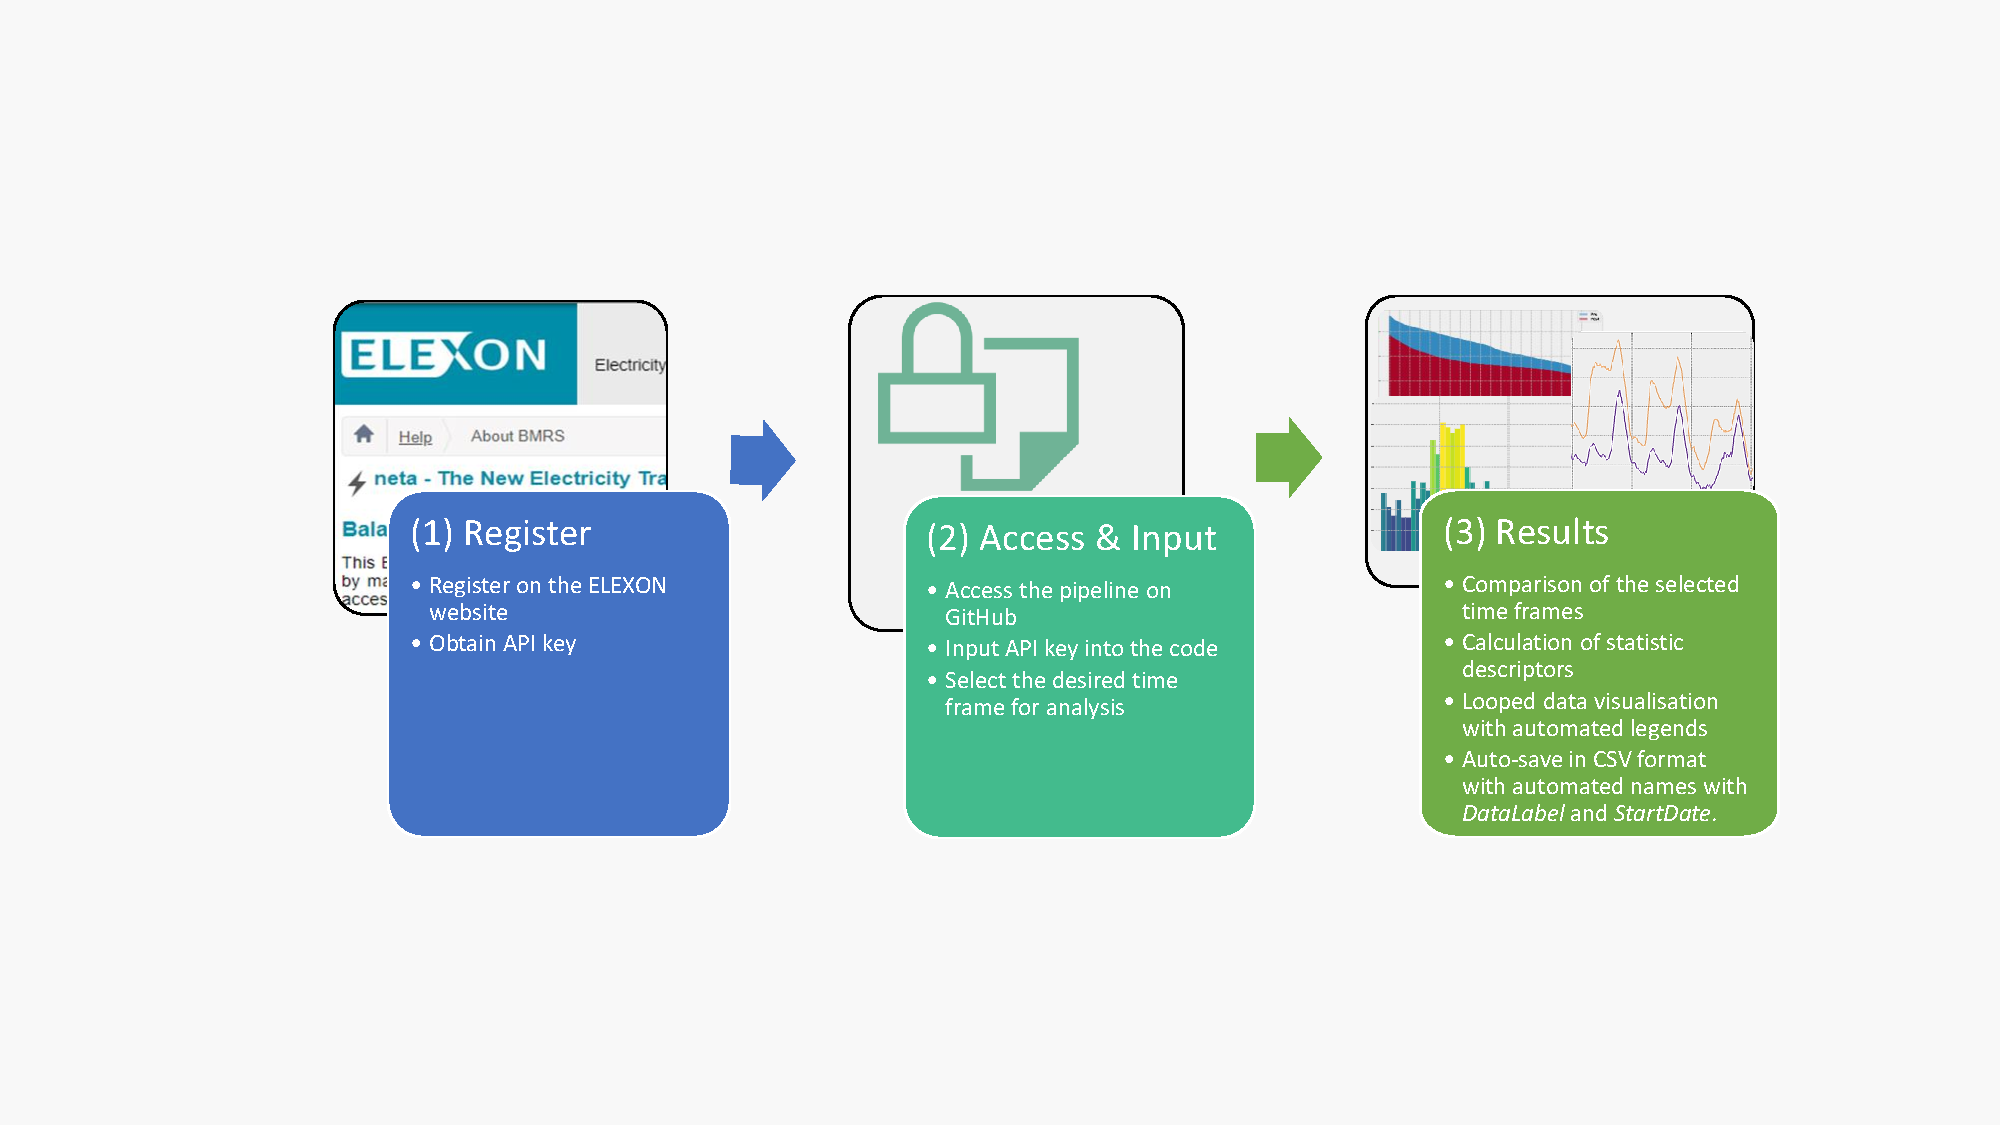
\includegraphics[trim={4cm 2.5cm 3cm 3cm}, clip, width=15 cm]{Graphics/Flowchart_pipeline.pdf}
\caption{The flowchart displaying the steps for employing the data pipeline.}\label{fig:pipeline_flowchart}
\end{figure}  

As shown in Figure \ref{fig:pipeline_flowchart}, there are 2 prior steps to reaching the results stage where the quantitative data descriptors are calculated and the results are visualised in a comparative manner. The first step is to obtain an API key by registering on the Elexon website \cite{ElectricityBMRS} - a more detail guidance on this is provided by Elexon \cite{Elexon2019BMRSArchitecture}. Then, the pipeline can be accessed from the GitHub website \cite{KirliElectricityPipeline} or Appendix \ref{section:PipelineCode} and the API key obtained by the user should be input. The default time frames are set to the pre and post-COVID-19 weeks used for this analysis which are weeks commencing on 2\textsuperscript{nd} and 23\textsuperscript{rd} of March 2020. However, these can be adjusted to the time frame of interest. In addition to the system demand, this pipeline can be used for all other data types provided by Elexon which are listed in \cite{Elexon2019BMRSArchitecture}. The code can also be modified to refer to any other website to execute a direct data extraction using API.





% \begin{theorem}
% \KwResult{Write here the result }
%      initialization\;
%      \While{While condition}{
%       instructions\;
%       \eIf{condition}{
%       instructions1\;
%       instructions2\;
%       }{
%       instructions3\;
%       }
%      }
%      \caption{How to write algorithms}
% \end{theorem}


%===============================================================
%                           RESULTS
%===============================================================

\section{Results \label{section:Results}}
In order to effectively present the impact of the COVID-19 lockdown on the GB electricity system, four main categories are identified and analysed: (1) the changes in demand profile and volume, (2) generation portfolio; renewable and conventional generation shares, (3) forecasting and grid stability indicators, and lastly (4) market prices, including day-ahead wholesale market, system imbalance and variable prices for the distributed consumers. Furthermore, the grid stability subsection inspects imbalance volume, system frequency and the loss of load probability. 

% Wherever possible, the results are presented in a quantitative manner. However, as it is often questionable or leading to distorted conclusion, when comparing only single weeks with completely different weather conditions (i.e. solar radiation, wind speed and temperature), a qualitative approach was chosen to complement the results.

%%%%%%%%%%%%%%%%%%%%%%%%%%%%%%%%%%%%%%%%%%

\subsection{Demand Profiles}\label{section: Effect on demand profile}

This subsection analyses and quantifies the changes in the electricity consumption caused by the COVID-19 mitigation actions such as the lockdown. On the 23rd of May, the UK Government recommended work from home (WFH) and closed public spaces such as pubs, restaurants and sport facilities \cite{GovernmentGOV.UK}. The impact on the electricity demand is shown by the purple profile and compared to a pre-COVID-19 week in Figure \ref{fig:demand_profiles}. The figure illustrates that the overall demand decreased as majority of the commercial users (e.g. factories, businesses, etc.) shut down.
Besides the demand reduction, the lock-down also influenced the consumption pattern which results in a changed load profile shape.
%Old alternative: Nevertheless, this increased the influence of the domestic consumption pattern that resulted not only in a decreased electricity consumption but also a changed profile shape.

\begin{figure}[H]
\centering
\hspace{-25pt}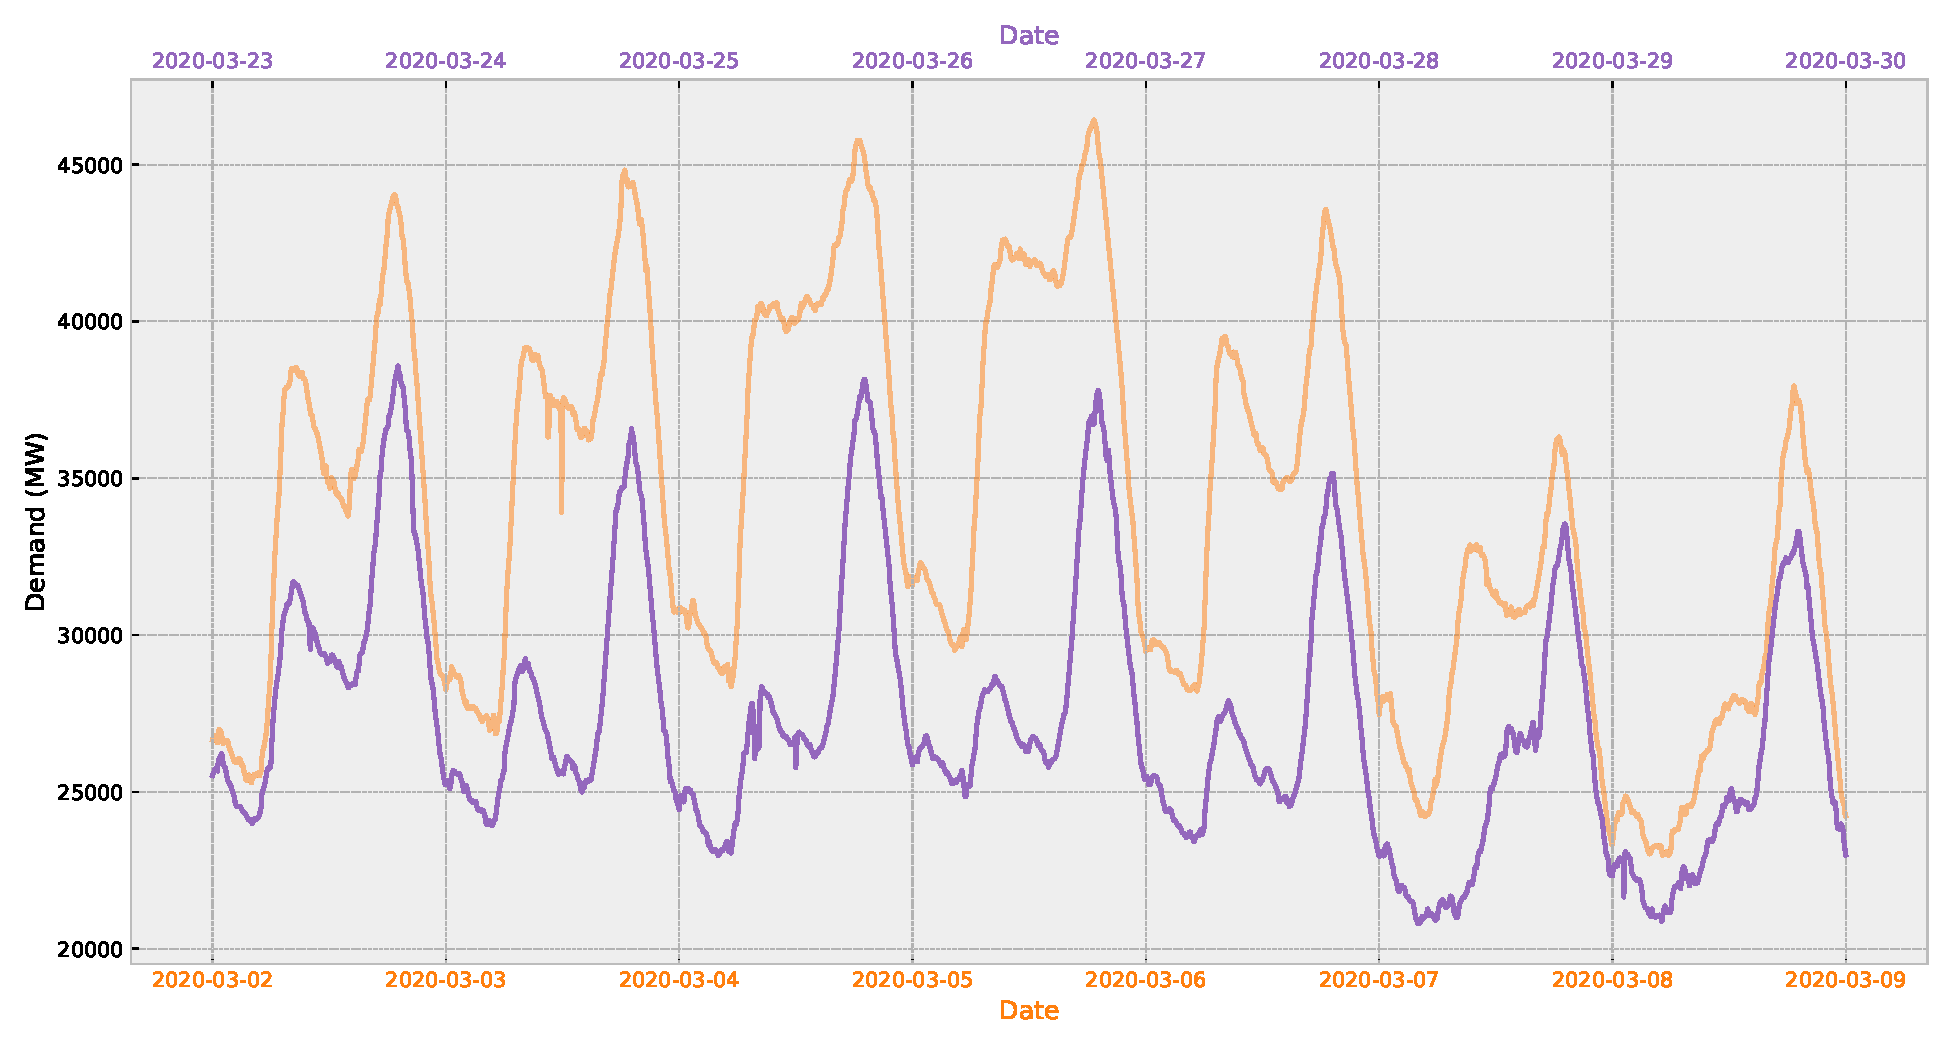
\includegraphics[width=15 cm]{Graphics/Demand_profiles.pdf}
\caption{Aggregated system demand before and after the COVID-19 actions}\label{fig:demand_profiles}
\end{figure}  

As displayed in Figure \ref{fig:load_duration}, load duration curves show the base and peak demand by visualising the relationship between sorted demand (i.e. ranked descending) and exceedence. Whilst the base demand decreases 10\%, the peak and mean demand drastically drop by 20\% and 24\% respectively, following the start of the lockdown. The changes in the demand profile for peak, mean and base load are shown in Table \ref{table:load-duration}. The decrease in the energy demand can also be observed as the area of the red plot (i.e. post-COVID-19) is smaller than the blue plot (i.e. post-COVID-19). If the demand constant that would result in a flat load duration curve. In Figure \ref{fig:load_duration}, the post-lockdown plot (in red) is flatter than the previous one. This is also supported by the higher decrease in peak values in comparison to the base. This indicates a significant change in the emand profile and that it is flatter than the pre-action one. Flattening the demand curve means the prime time peaks such as the morning pick-up and the evening demand surge are now less pronounced. Such peaks increase the difficulty of matching demand and supply, puts the grid under stress and also increases the stress on thermal generation and storage to meet the demand. The ripple effects include congestion and high imbalance and transmission charges. 
%General Note: visualise the relationship between sorted demand (i.e. ranked descending) and time. %It is used to analyse the variation in energy (i.e in Figure \ref{fig:load_duration}, the area of the graph gives the energy used in MWh) and choose baseload and peak load power for generators. 

\begin{figure}[H]
\centering
\hspace{-25pt}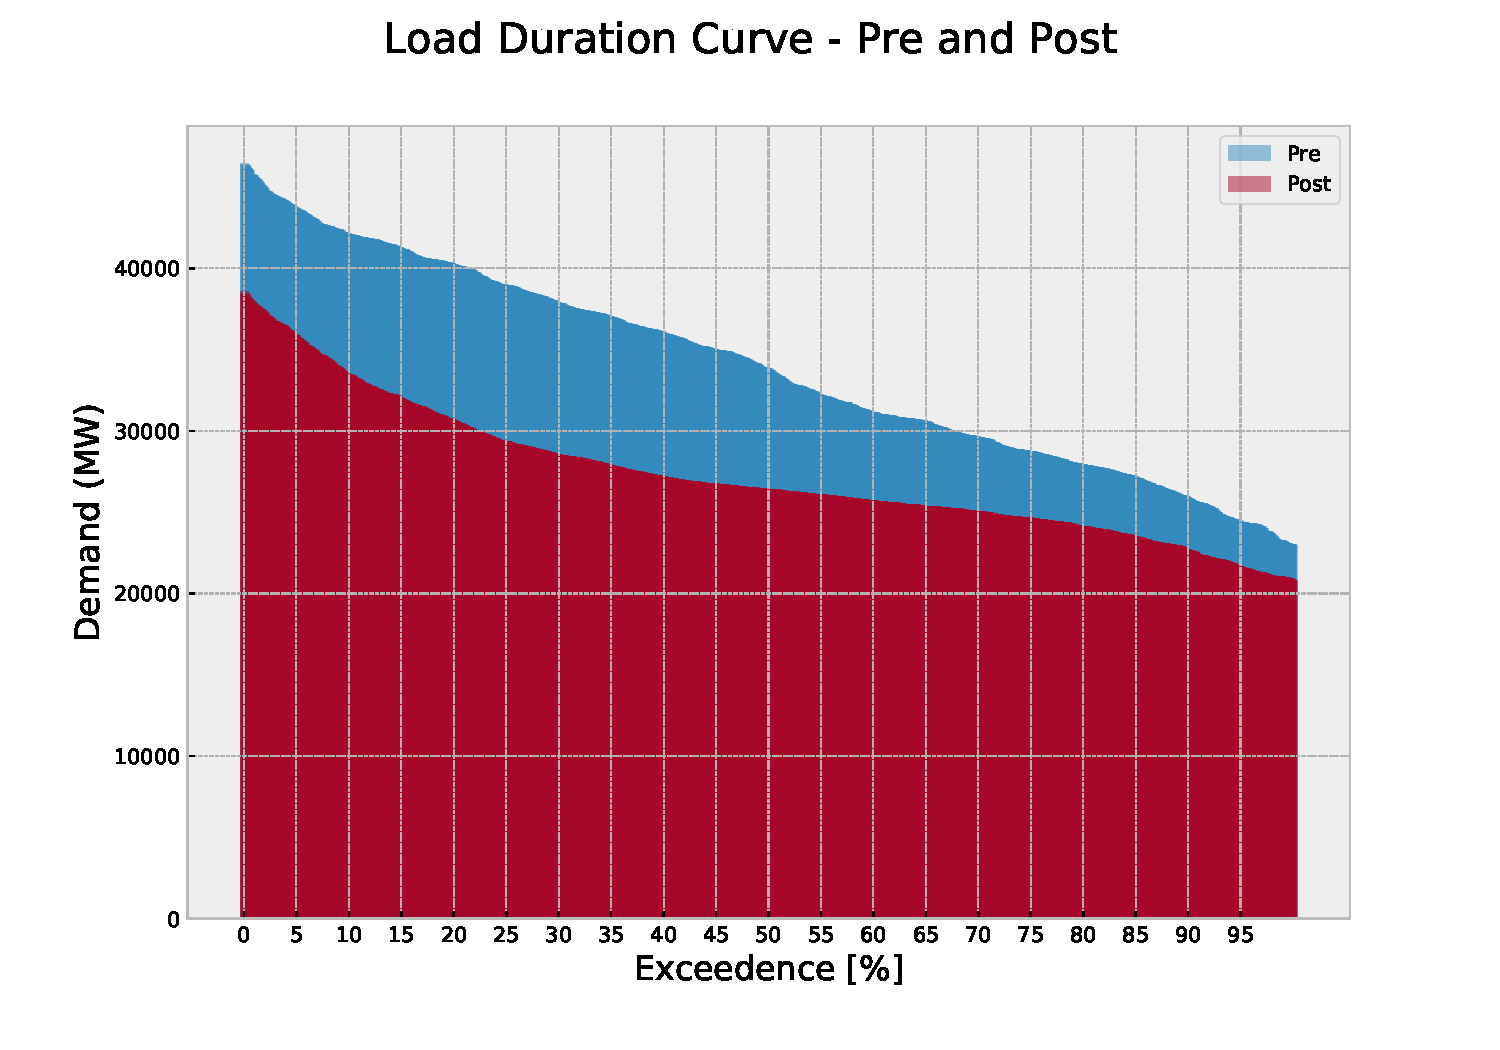
\includegraphics[width=13 cm]{Graphics/Load_duration_curve.pdf}
\caption{Load duration curve for pre- and post-COVID-19 actions.}\label{fig:load_duration}
\end{figure}  

\begin{table}[H]
\caption{Changes in demand profile using the data from the load duration curves. }
\centering
%% \tablesize{} %% You can specify the fontsize here, e.g., \tablesize{\footnotesize}. If commented out \small will be used.
\begin{tabular}{ccccccc}
\toprule
\textbf{Profile} & \textbf{Peak Load (MW)}	& \textbf{\%} & \textbf{ Mean Load (MW)}	& \textbf{\%}	& \textbf{ Base Load (MW)}	& \textbf{\%}\\
\midrule
Pre	& 46425 & & 33868 & & 22982 &  \\
Post & 38585 & \textcolor{red}{-20.31\%} & 27294 & \textcolor{red}{-24.08\%} & 20795 & \textcolor{red}{-9.5\%} \\

\bottomrule
\end{tabular}
\label{table:load-duration}
\end{table}






T, Figure \ref{fig:Demand_hist} shows the demand histogram shifted to the left, indicating lower loads. The lighter colour (i.e.mostly yellow) peak for the post-action demand show that the range of most occurring demand values is now narrower, meaning there is less variation. Otherwise, the pre-action demand shows a more disperse and even occurrence profile which looks slightly bi-modal. The bi-modality, meaning that two occurrence centres exist. 

% DKComment: not sure if this is written about the right figure. While during non-work hours the profile is levelled on the base load and work-hours show another load centre. In conclusion, the effects taken after the COVID-19 actions denoting a higher occurrence of lower demands which results in a smoother load profile.



\begin{figure}[H] 
\centering
\hspace{-25pt}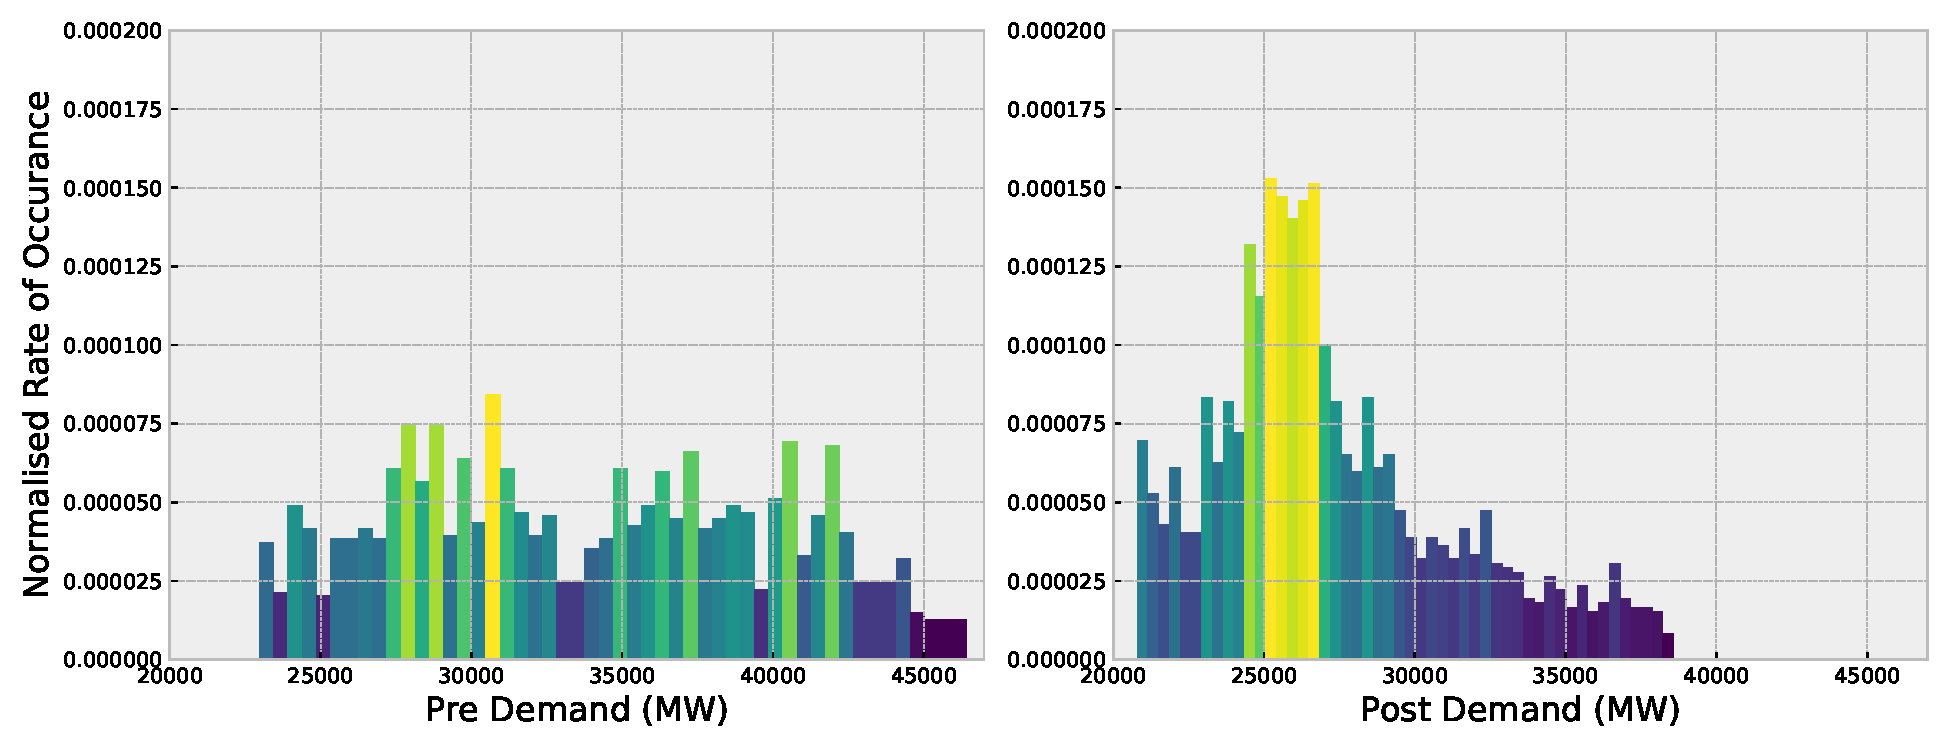
\includegraphics[width=16.5 cm]{Graphics/Demand_hist_coloured_sidebyside.pdf}
\caption{Comparison of pre- and post-COVID-19 demand histograms with normalised occurrences. The range of colours from yellow to dark blue correspond to the highest and lowest values.}\label{fig:Demand_hist}
\end{figure}  


% \textcolor{purple}{
% \textbf{Quick Results so far}
% \begin{itemize}
%     \item 1 hour shift in "morning peak" - 9 am to 8 am and "evening peak" - 6 pm to 7 pm
%     \item Steeper climb to the "evening peak" - used to be 7500 MW increase over 4 hours, now it is 9500 MW increase in 5 hours.
%     \item Overall decrease in Peak-to-Mean ratio -except  7, 8, 9 am. However, it seems to follow the same morning trend as the pre data which had its max PtM value at 6 am at 0.18. This peak is delayed to 8 am and decreased by 1. 
%     \item Speculation: People wake up later, cook earlier - change in heating demand.
%     \item Standard deviation is smaller by a third of its original value (i.e. 6085). Presumably, this could explain the better performance of forecasting algorithms.
% \end{itemize}
% }
Figure \ref{fig: var_dem} uses a ratio of standard deviation to mean in order to quantify the variation in the consumption profile. It suggests an overall lower variation in the post-COVID-10 profile with a largest variation in the morning with respect to the mean. The evening variation coefficient is also remarkably lower. The overall standard deviation of the post-lockdown week is a third of the pre-lockdown week. Hence, it also connotes to the discussion of the flatter demand profile. Figure \ref{fig: var_dem} also reflect an hour delay in the morning peak (i.e. 8 to 9 a.m.) and a changed evening profile. Regarding the evening demand surge, it should also be noted the Figure \ref{fig:demand_profiles} also the post evening peaks are steeper in comparison as the morning peaks become less pronounced. For instance, on average the pre demand used to have a 7500 MW increase over 4 hours to the evening peak whereas the post-action demand escalates by 9500 MW in 5 hours. Despite the longer increase time, the relative increase is higher.


\begin{figure}[H]
\centering
\hspace{-25pt}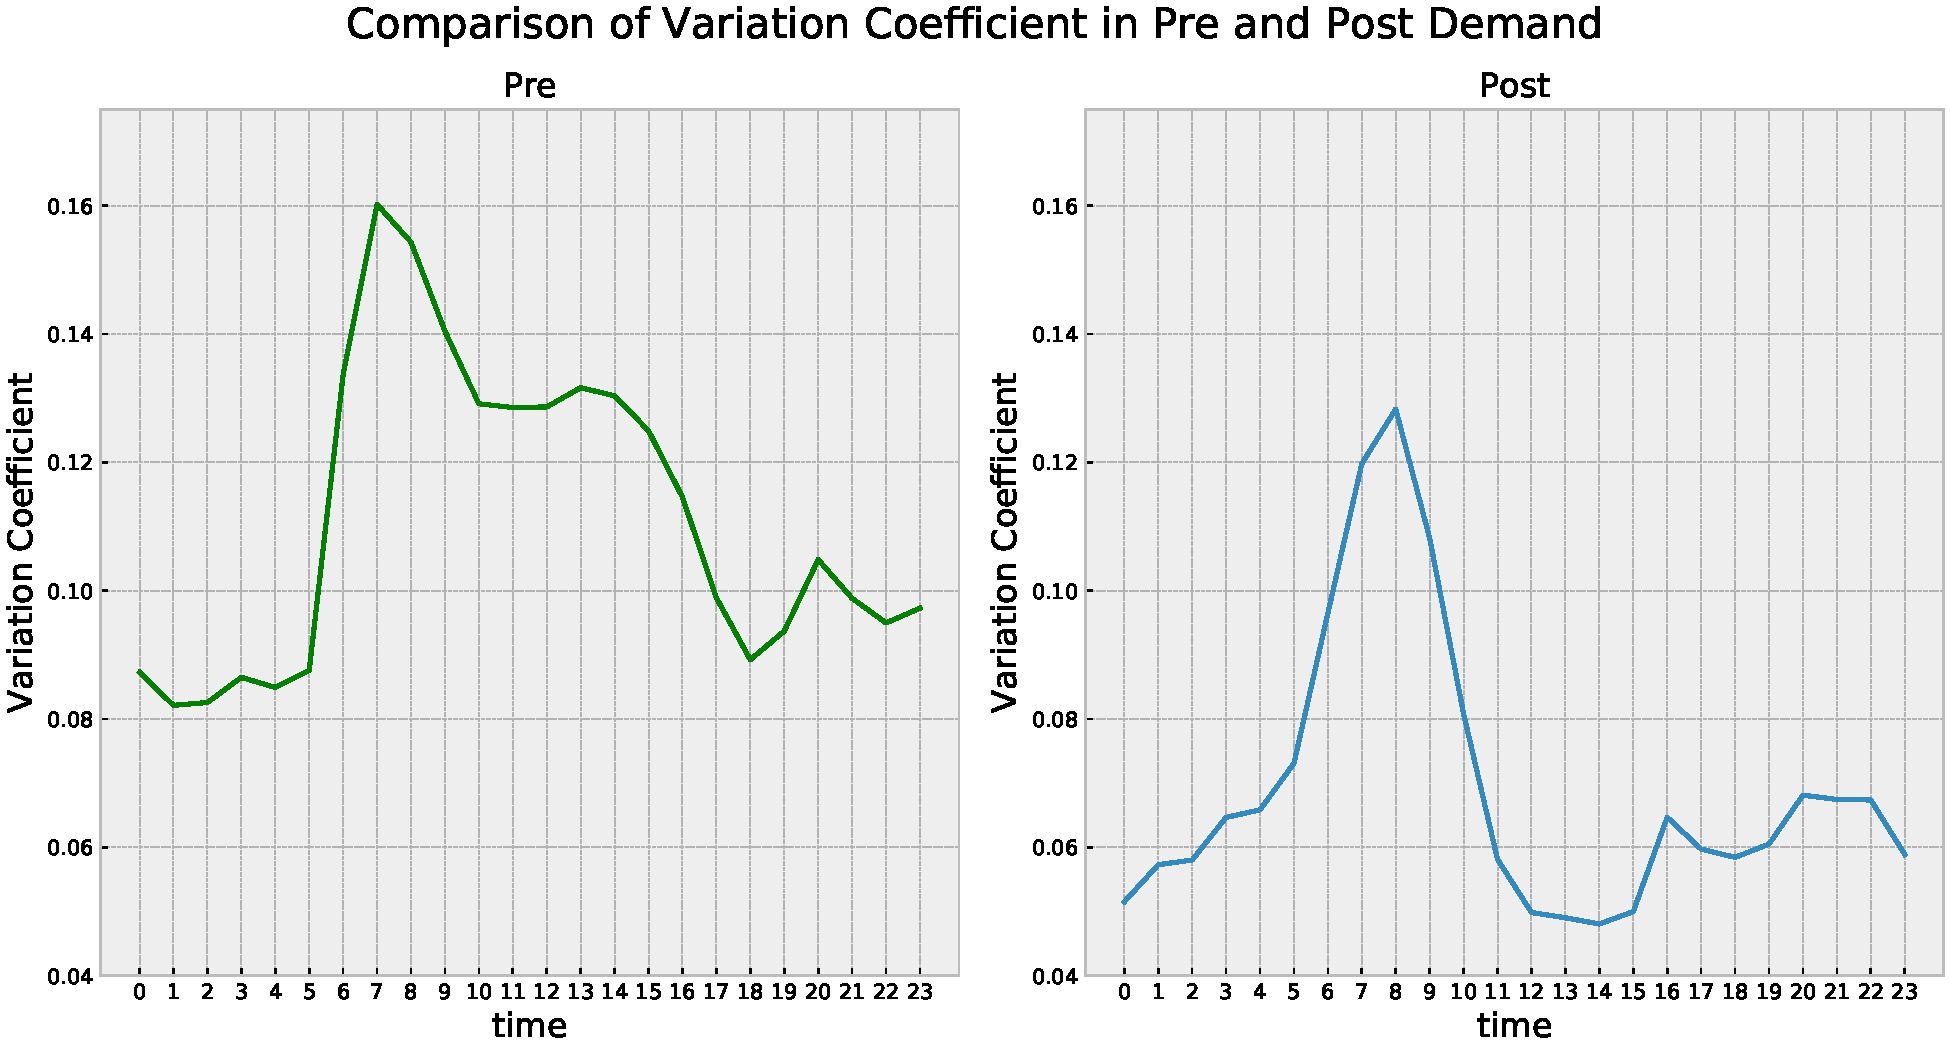
\includegraphics[width=14 cm]{Graphics/VarCoeff_comp.pdf}
\caption{Comparison of variation coefficient to visualise the changes in system demand.}\label{fig: var_dem}
\end{figure}  

It could be speculated that this is due to the human behaviour change as the common 9 a.m. to 5 p.m. working routine may not apply to all WFH. Hence, the delay in the morning peak may suggest a later wake-up time and earlier pick-up in the evening may connote to earlier increase in heating demand, cooking and similar.

% \begin{figure}[H]
% \centering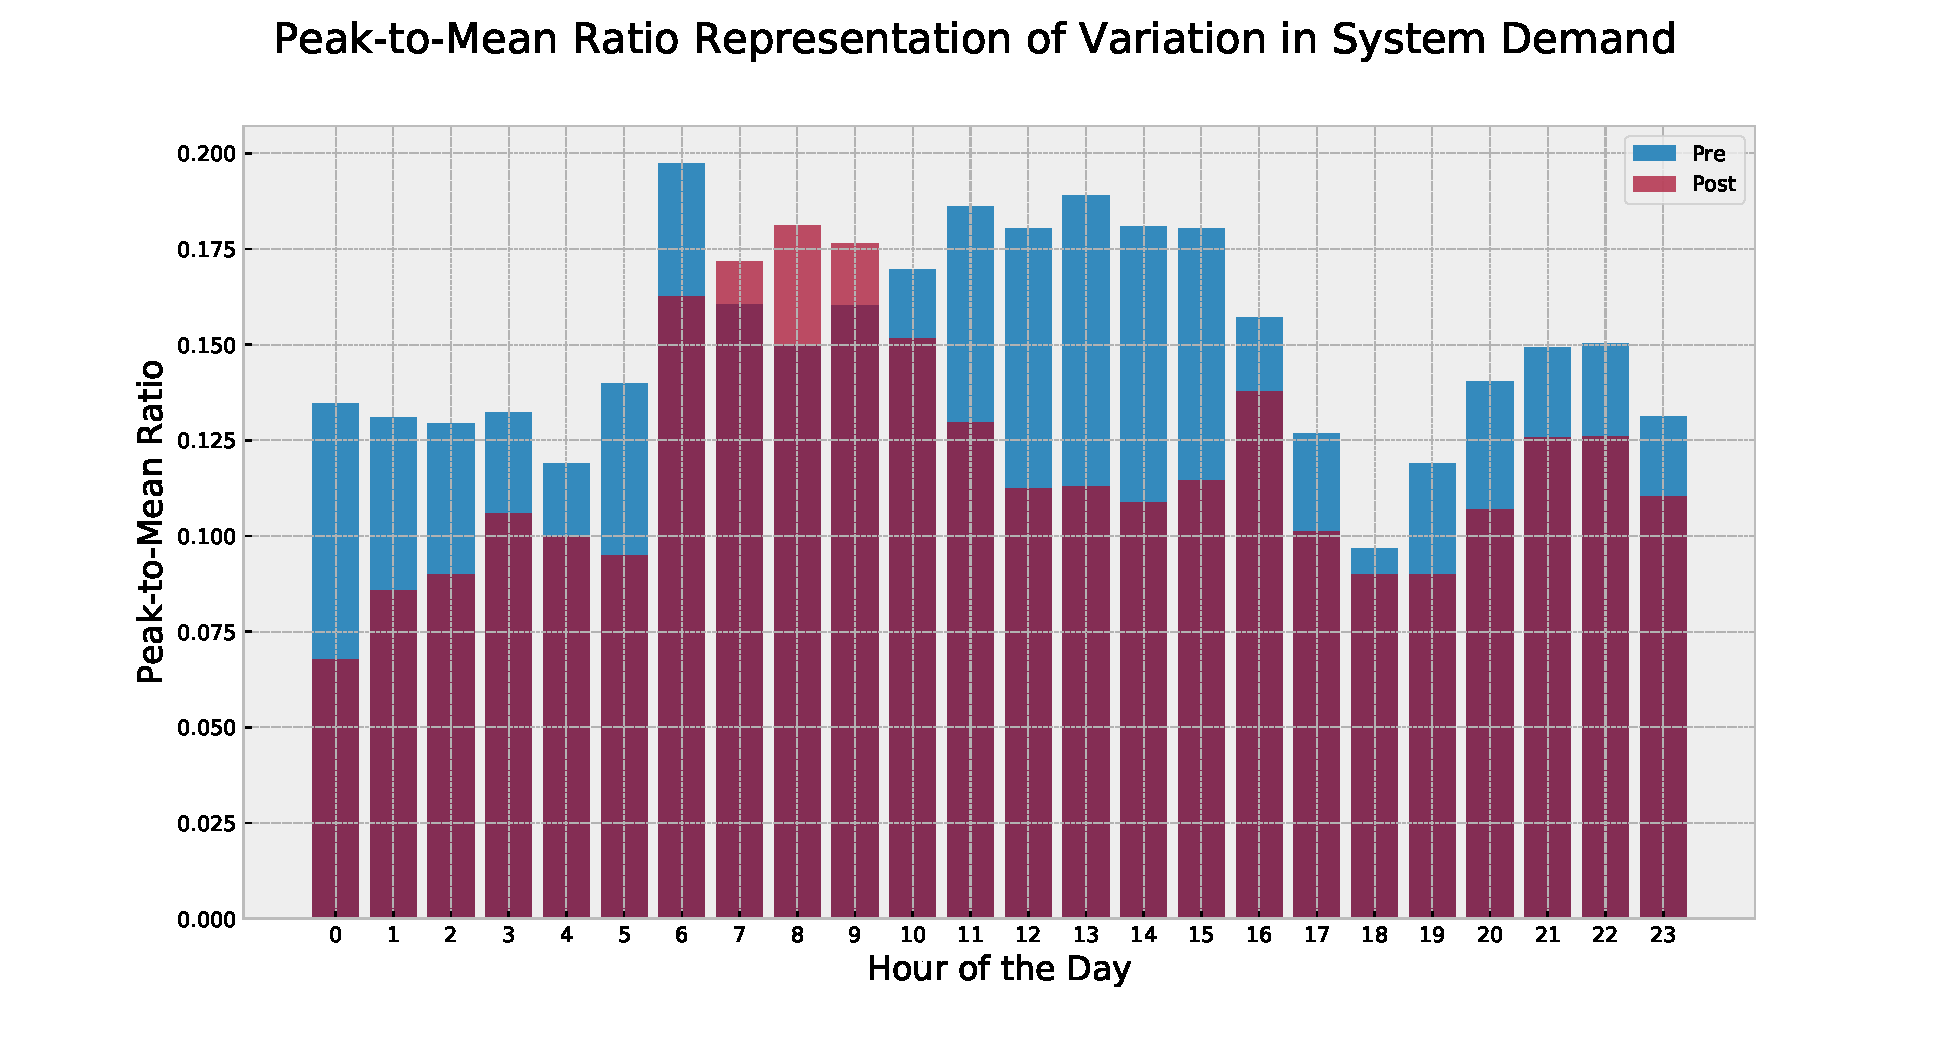
\includegraphics[width=17cm]{Graphics/PtM_ratio_Demand.pdf}
% \caption{Overlaying the peak-to-mean ratios to compare the variation in system demand.}\label{fig: PtM_Ratio_Demand}
% \end{figure}


% \begin{figure}[H]
% \centering
% \hspace{-25pt}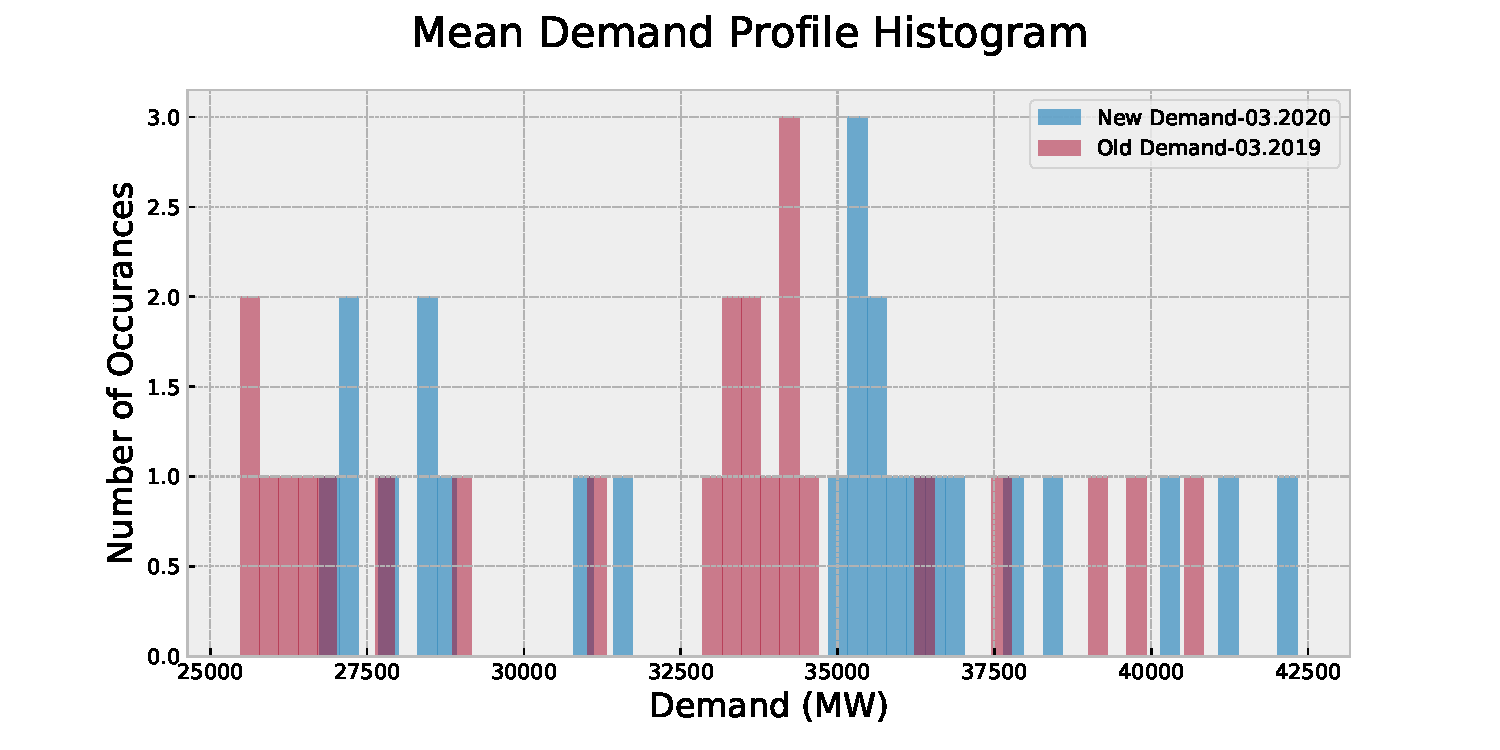
\includegraphics[width=16.5 cm]{Graphics/Mean_Demand_Profile_hist.pdf}
% \caption{}
% \end{figure}  



% \begin{table}[H]
% \caption{Comparison of statistical descriptors to quantify the changes in the demand pre- and post-COVID-19 mitigation actions. }
% \centering
% %% \tablesize{} %% You can specify the fontsize here, e.g., \tablesize{\footnotesize}. If commented out \small will be used.
% \begin{tabular}{cccc}
% \toprule
% \textbf{Demand Data} & \textbf{Coefficient of variation}	& \textbf{Peak-to-mean ratio}	& \textbf{Inter-quartile range}\\
% \midrule
% March 2019		& data			& data         &data\\
% March 2020		& data			& data         &data\\
% Other years also&data          &data           &data\\
% \bottomrule
% \end{tabular}
% \end{table}

%%%%%%%%%%%%%%%%%%%%%%%%%%%%%%%%%%%%%%%%%%%

\subsection{Generation Portfolio}\label{sec:Generation portfolio}
This subsection focuses on how the changes in demand pattern and magnitude affected the generation portfolio. In particular, the lower demand lead to a higher share of variable renewable energy (VRE), namely wind and solar, and consequently impacted the conventional generation portfolio in the power system. 

\subsubsection{Increase in renewable energy contribution}
The share of generation from VRE sources increased following the COVID-19 mitigation actions and consecutive changes in the electricity demand. The hypothesis for this originates from the causality principles in electricity markets which is further supported by an example. 
Firstly, generators in European electricity markets are scheduled in merit order, which means that the generators with the lowest marginal costs are supplying the power demand. The causality is that the VRE generators have marginal costs close to zero. Therefore, the VREs are usually scheduled before other generation technologies \cite{Winkler2016ImpactMatter}. As the VRE infrastructure already exists, is preferred in the merit order and the VRE output is not restricted by the pandemic circumstances, it is justifiably hypothesised that the changes in the demand profile and magnitude resulted in the increase of the VRE contribution. 

Secondly, to support this hypothesis it must be noted that, besides the total generation or load, the VRE share also depends on the weather conditions which impact the VRE output in every point in time. Changing weather conditions make it hard to compare pre and post-COVID-19 data sets as it is not possible to decouple the effect of weather conditions and the VRE generation. This is because the aggregated VRE output from various locations is used for this study. Therefore, Figure \ref{fig:generation_effects} illustrates a qualitative example which keeps the VRE generated output stable (i.e. unaffected by varying weather conditions), representing constant solar and wind conditions for a high and low demand case, respectively. 
The scale for demand and generation in Figure \ref{fig:generation_effects}, represents approximately real observed data from GB \cite{ENTSO-E2020ENTSO-EPlatform}. In the example, the demand reduction of 25 \%, which was recognised in the first week after the lock-down, lead to an absolute VRE share growth of 8 \%.

As result of Figure \ref{fig:generation_effects} and the preference of scheduling VRE before conventional generators, the average demand reduction lead to higher VRE shares in long-term. If the data from Figure \ref{fig:generation_effects} is representative for more periods, it further indicates that the VRE share could increases in the range of 5-10 \% in the GB system due to the lower demand profile.


\begin{figure}[H]
\centering
\hspace{-25pt}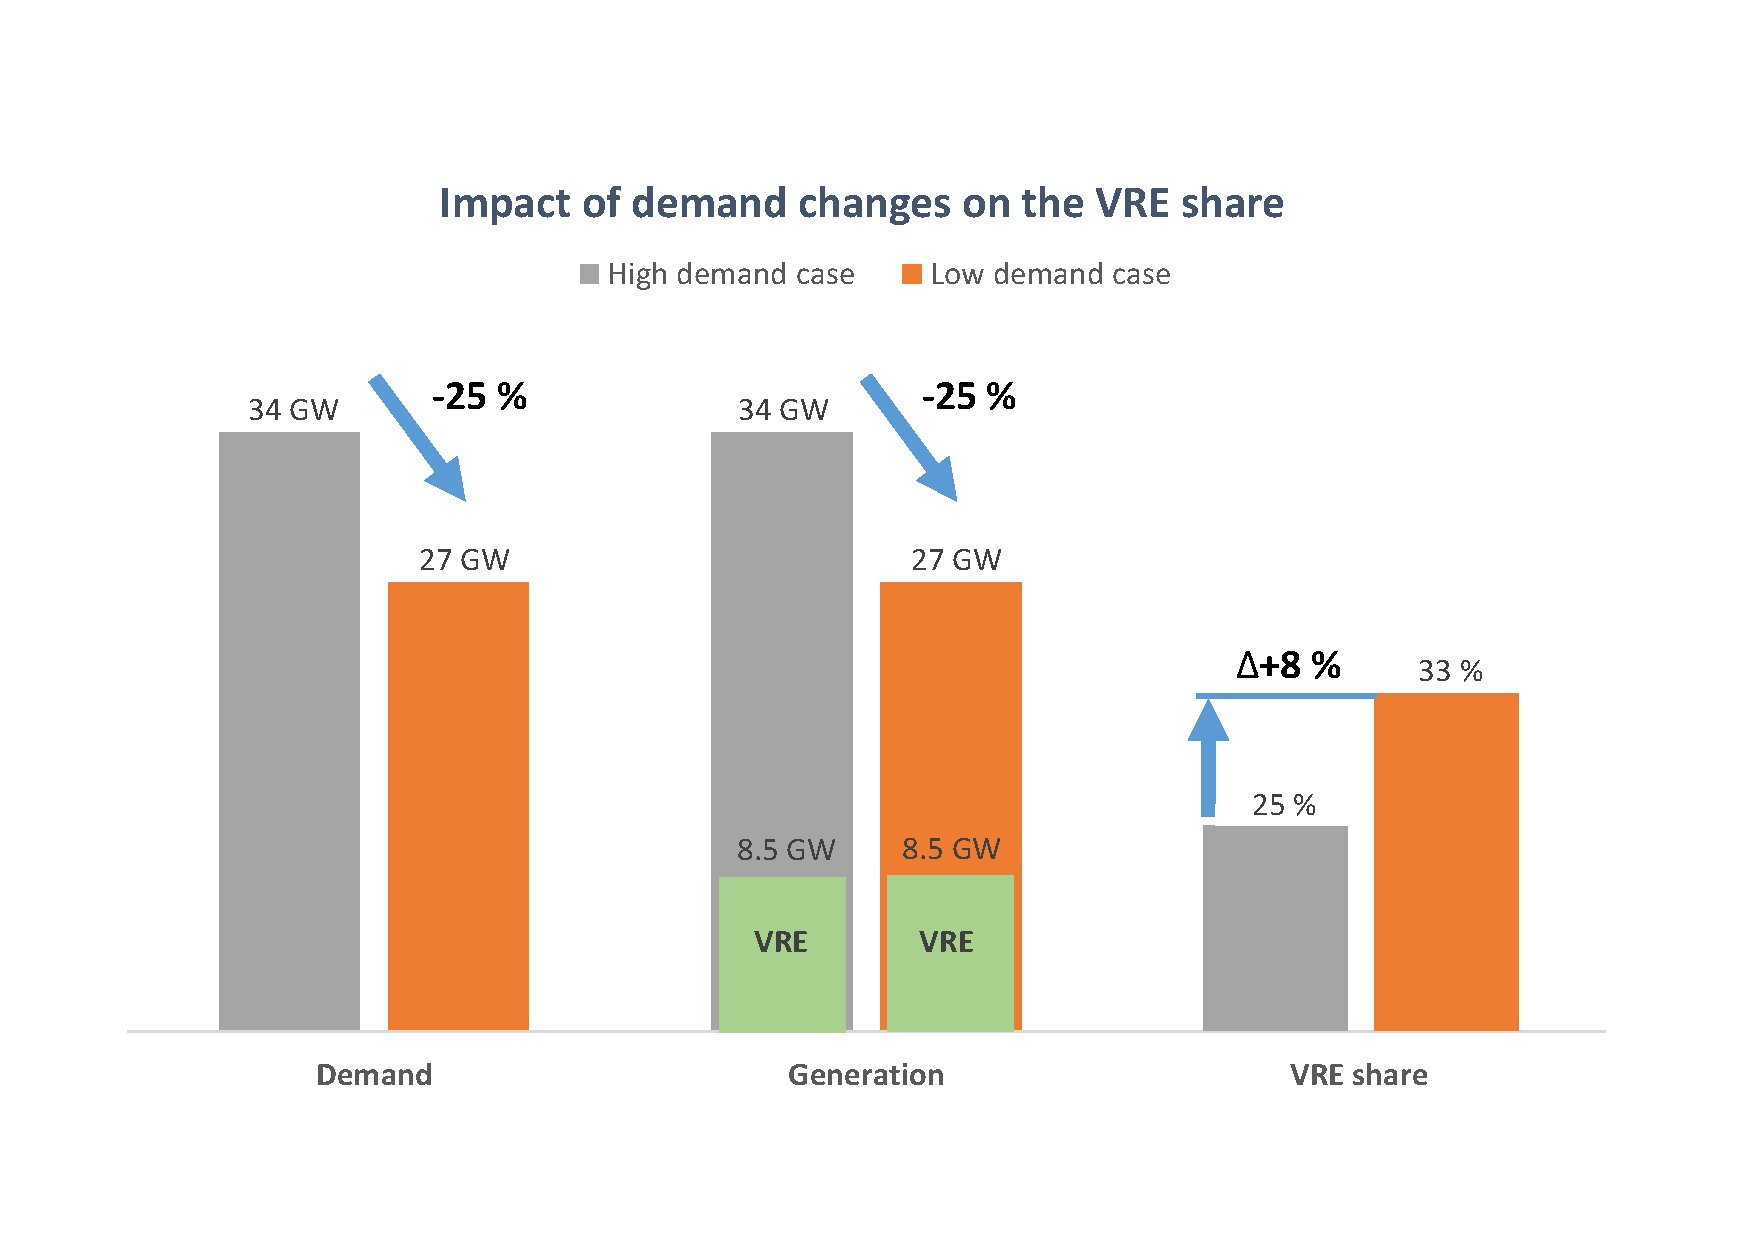
\includegraphics[trim={0cm 2cm 0cm 2cm},clip,width=1\textwidth]{Graphics/Illustrative-VRE-share-increase2.pdf}
\caption{A qualitative example of the impact of demand changes on the VRE share. Share of VRE share, and ratio of demand changes equal roughly the UK case, check \protect\cite{ENTSO-E2020ENTSO-EPlatform} and section \protect\ref{section: Effect on demand profile}, respectively.} %DKComment:Need to update the caption
\label{fig:generation_effects}
\end{figure} 

%DKComment:Should we talk about how these are low-carbon technologies and how this aids with meeting the green generation goals - eventually helping fight climate change. Perhaps, we leave this to the Discussion bit.

\subsubsection{Impact on the conventional generation portfolio}
%DKComment:It might be worht mentioning at the top perhaps that behind-the-meter VRE generation is not included in this - and that the effect of increased VRE can even be bigger than we estimate.

The conventional generation portfolio, including all generation assets with marginal cost above solar and wind technologies, are expected to decrease in operation time compared to the situation without lock-down. The reason is beside the lower total demand, the higher share of VRE assets on the market which are dispatched first because of the merit order. The decrease of operation time will particularly effect higher marginal cost generators, so that nuclear and hydro plants are less effected. However, the higher share of VRE assets cause additionally a need for more flexibility in the power system - such as provided from the natural gas plants \cite{Hirth2014TheVariability}. If inflexible plants are not willing to reduce their generation at high VRE times, the more often negative prices will occur \cite{IEA2016Re-poweringSystems.,Cochran2013MarketSystems}. Therefore, a flexible gas or biomass plant could be preferred over a less flexible coal plant. 

As result, the total generation portfolio is likely to reduce carbon emissions by the increase of the VRE share and the push out of inflexible coal plants.
%DKComment:what about Hydro, Nuclear, etc. - perhaps it is good to categorise a bit here as high, med and low carbon tech.
%MPComment: Not sure 

%Therefore, the question arises how to compare the VRE share for two weeks with different VRE potential. The answer is factorising both weeks to each other.
%In Figure \ref{fig:generation_effects}, a pre-COVID week was factorised with a post-COVID week for the absolute VRE generation and the total VRE share in the power system. When looking on the lock-down day, the VRE generation increased from pre- to post COVID week by 126 \%, while the total VRE share increased by 169 \%, which result in a difference of 43 \%. On typical days the percentage difference might vary in small ranges as new VRE capacity might be added to the power system or due to load variations. Otherwise, the lock-down lead to a drastic lower demand profile, which increased the percentage difference over-proportional. One could question why in Figure \ref{fig:generation_effects} the percentage difference on Sunday is low. One reason is that on a typical Sunday most businesses are closed and therefore the load profile doesn't vary too much from COVID load profile. In conclusion, the observed data can interpreted as evidence that the lower demand leads to a higher share of VRE in the power system. 

%\begin{figure}[H]
%\centering
%\hspace{-25pt}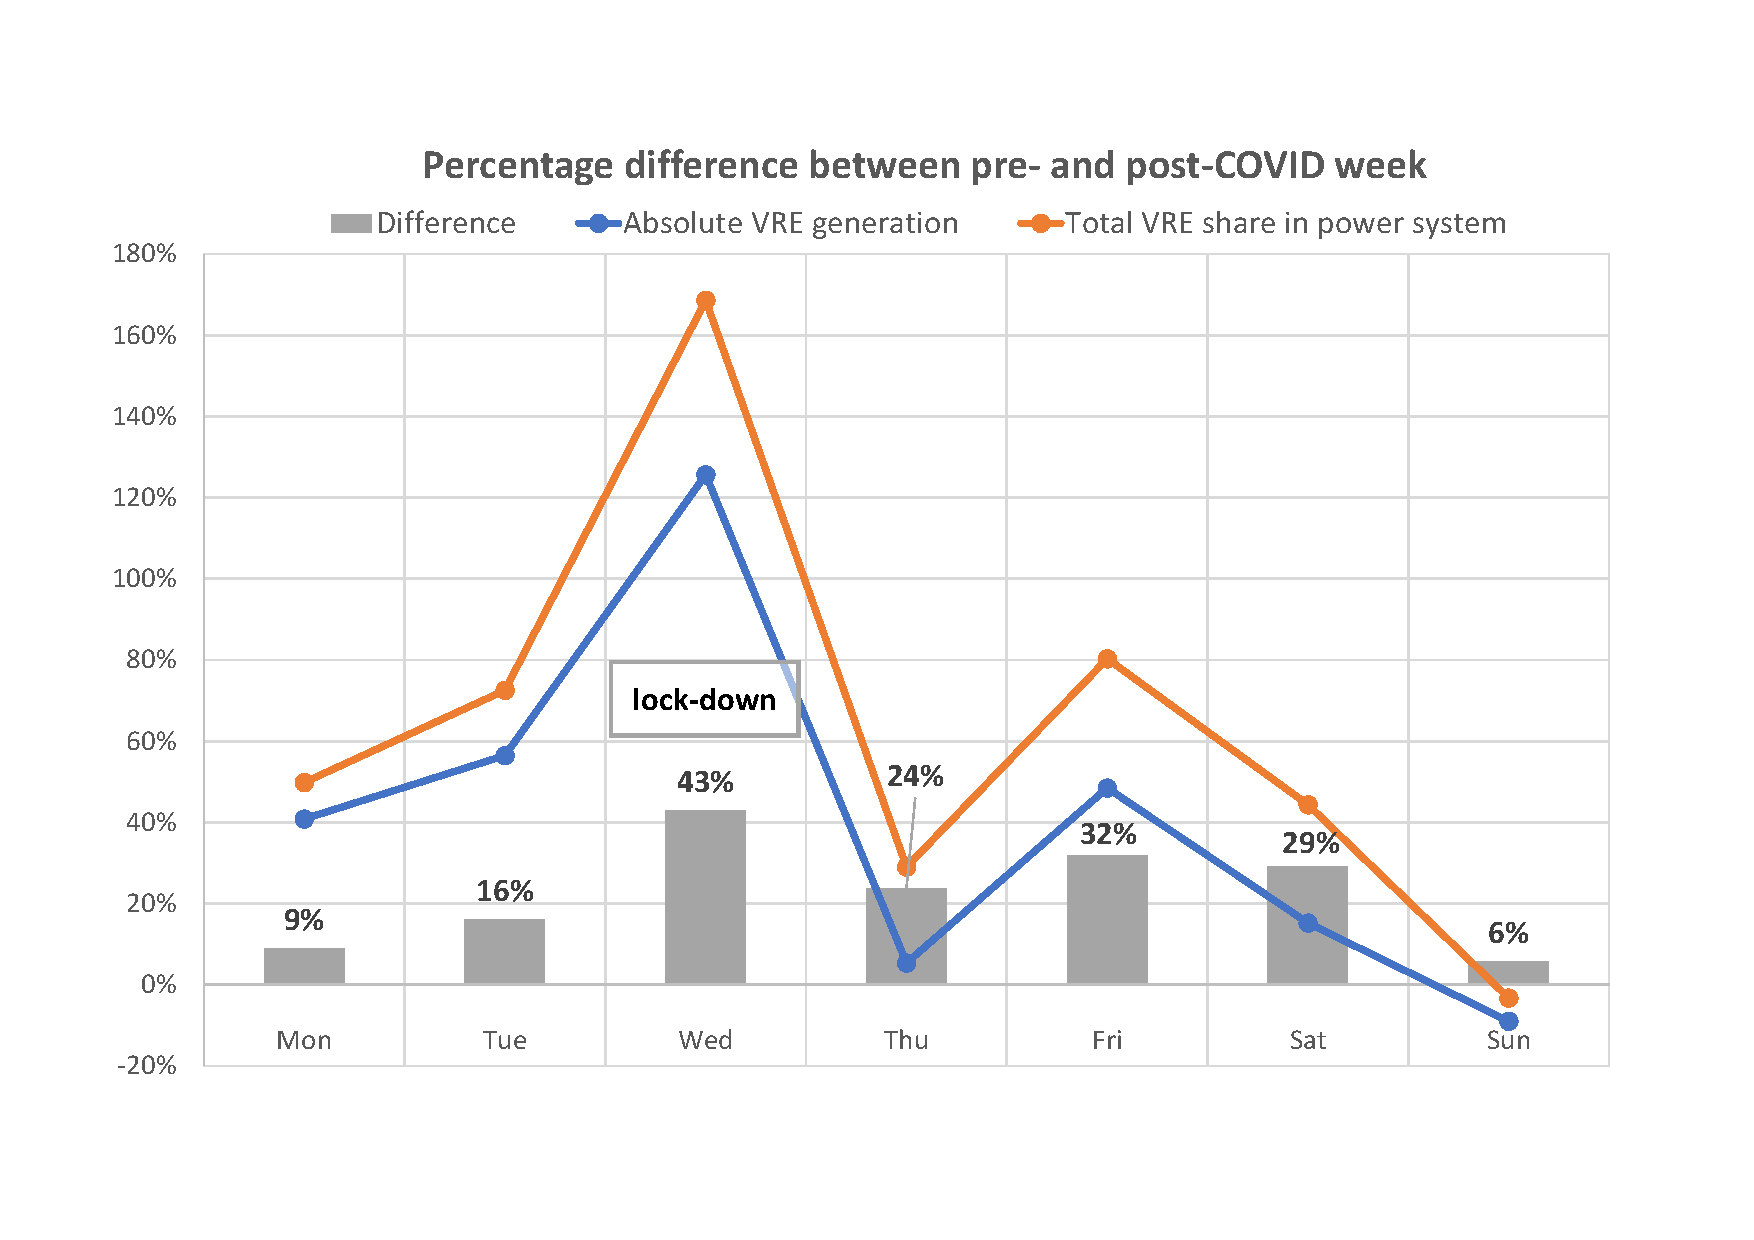
\includegraphics[trim={0cm 2.5cm 0cm 2.5cm},clip,width=1\textwidth]{Graphics/Weather-independent-VRE-Share-increase.pdf}
%\caption{Percentage difference for i) VRE generation and ii) VRE share in the power system in the pre- and post-COVID week, 02-09 March and 22-28 March, respectively. While zero percentage represent the pre-COVID daily baseline, the coloured points represent a grow or decrease factor for the post-COVID week. Data extracted from ENTSO-E transparency platform \protect\cite{ENTSO-E2020ENTSO-EPlatform}.}
%\label{fig:generation_effects}
%\end{figure} 

%%%%%%%%%%%%%%%%%%%%%%%%%%%%%%%%%%%%%%%%%%%%%%%%%%%%%%%%%%%%%%%%%%%%%%%%%%%%%%%%%%%%%%
\subsection{Forecasting and Grid Stability}
The aspects related to forecasting and grid stability are discussed in this section. These include factors such as the deviations in system frequency, imbalance volume and load forecast error of the system operator. Additionally, it investigates the loss of load probability as indicators of the reserve scarcity and increased stress in the grid.

\subsubsection{Load Forecast Error}\label{DemandForecastError}
The effect of COVID-19 on the short-term load forecasts are analysed in the GB power system. In contrast to mid- and long-term forecast, which make predictions months and years prior to the event, the short-term load forecast have a shorter outlook which range from one hour to weeks before the settlement period \cite{SahayDayNetwork,Khuntia2016ForecastingReview}. Short-term load forecasting plays an important role in scheduling the power plants efficiently in electricity market, as it is essential for economic dispatch and unit commitment \cite{He2020Day-aheadForest}. As a result, an improved forecast accuracy leads to a more reliable and affordable power system \cite{SahayDayNetwork}. 

Two different short-term load forecast are analysed in this study, the day-ahead total load forecast (DAF) and transmission system final load forecast (TSF). The DAF and TSF differ in methodology and forecast length. With regards to the methodology, the DAF represents a forecast for the total load in the power system, which equals the sum of generated power on both, transmission and distribution networks \cite{ENTSO-E2020ENTSO-EPlatform}. Whereas, TSF is a load forecast which is equal to the sum of generation present on the transmission network. However, this includes generation from pumped hydro storage and embedded large power plants on the distribution network level \cite{NationalGrid2020THE40}. Therefore, TSF is interpreted as the net demand, usually published by the TSO for market clearing, while the DAF represents the estimated actual total load in the power system.
%DKComment: Is it ok to say that TSF is required by TSOs and DAF is calculated for all loads present. I think we need to re-write the sentence above for clarity
%MPComment: Done
Regarding the forecast length, which is the duration from forecast publication till operation time, it varies for DAF and TSF, see Figure \ref{fig:forecast_length_explanation}. DAF is published only once a day and predicts the next-day average demand in each settlement period, hence, the forecast length vary from 12-36 hours \cite{ENTSO-E2020ENTSO-EPlatform}. Similarly, TSF outputs a day-ahead forecasts. However, forecasts for each settlement period is updated until the final TSF which predicts the next average demand in the next settlement period, 1 hour and 15 minutes ahead \cite{ELEXON2020ELEXONBMRS}.


%DKComment: Perhaps, it is better to change the source from ENTSOE to Elexon as we are using their data - right?
%MPComment: I used for the actual total load the ENTSOE data. Which is equal to the Elexon data, hence they report to ENTSOE
\begin{figure}[H]
\centering
\hspace{-25pt}
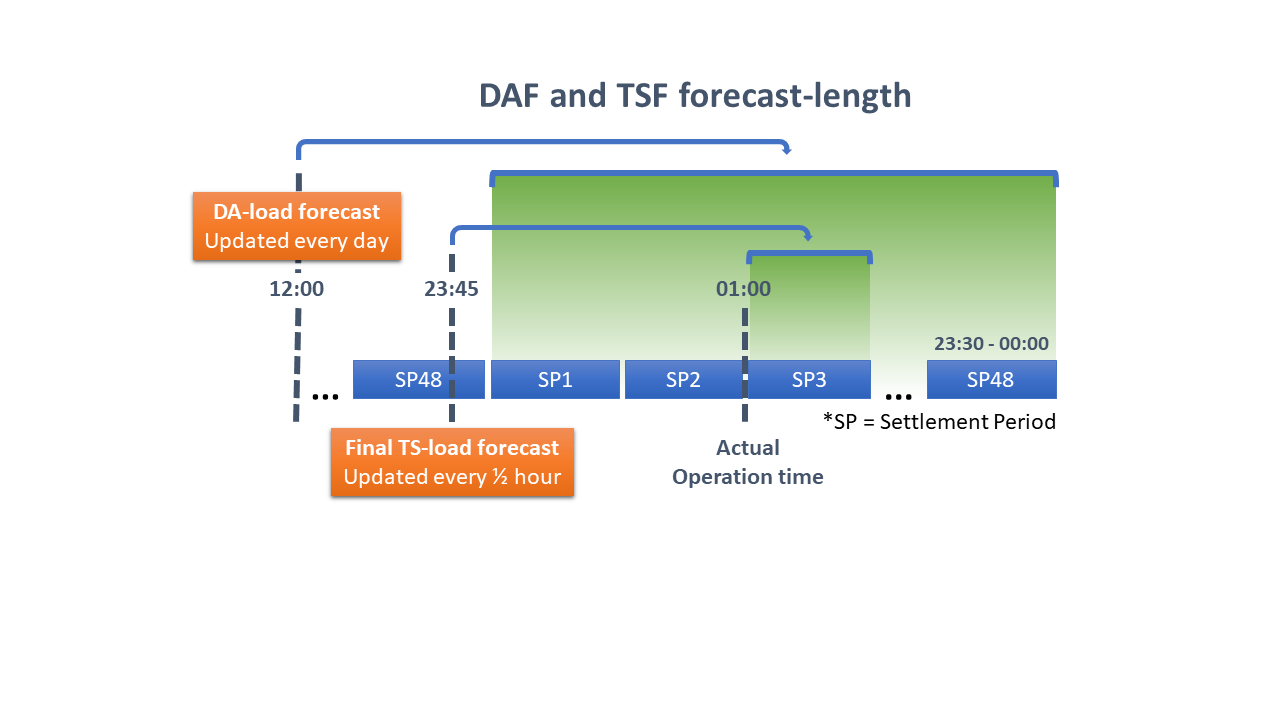
\includegraphics[trim={2cm 5cm 2 2cm},clip,width=1.1\textwidth]{Graphics/Forecast explanation.png}
\caption{Illustrative forecast lengths for the total Day-Ahead load forecast (DAF) and the final transmission system load forecast (TSF).}
\label{fig:forecast_length_explanation}
\end{figure} 

DAF and TSF forecast errors reveal different characteristics due to the lock-down. The DAF forecast is improved while the TSF forecast does not reflect clear changes. This is shown in Figure \ref{fig:DAFandTSFerror}. The forecast error is evaluated by one of the most common performance indicators, namely the mean absolute percentage error (MAPE) \cite{SahayDayNetwork, He2020Day-aheadForest}. MAPE functions well as a forecast performance indicator when employing historical data. Nevertheless, for prediction model selection and estimation it is biased \cite{Tofallis2015AEstimation}. As only historical data is analysed in this study, this makes MAPE a suitable indicator.
%DKComment: interesting comment about MAPE, not sure if we need to mention the bias about MAPE as it doesn't affect us - it can stay in I guess.
MAPE is defined as a summation of forecast errors, where each error is weighted to the actual load. This is shown in Equation \ref{eq:MAPE} where $y$ represents the actual load, $\hat{y}$ is the load forecast and $N$ is the number of forecasts.

%DKComment: Inserted an equation here to follow the journal's guidelines, commented out the text below. Could you please complete the sentence above just to make it clearer to the readers?

\begin{equation}\label{eq:MAPE}
MAPE = \frac{1}{N} \sum_{i=1}^N \frac{y_{i,actual} - \hat{y}_{i,forecast}}{y_{i,actual}}
\end{equation}

% \[ MAPE(\%) = \frac{1}{N} \sum_{i=1}^N \frac{y_{i,actual} - \hat{y}_{i,forecast}}{y_{i,actual}} \]

In general, the longer the forecast length is for the same point in time, the higher the forecast error becomes \cite{NationalgridESO2018QuarterlyMarch18}. 
%DKComment: I got confused by the same time resolution, do we mean for the same settlement period/time frame..i.e. same point in time?
%MPComment: Thanks
Therefore, the DAF constitutes a higher forecast error than the TSF. With regards to the lock-down effects, the improved forecast accuracy for the DAF is especially remarkable when distilling the time frame on the weekdays from Wednesday to Friday, which is time frame when the lock-down was initiated. The typical working week differs from the lock-down working week, and the weekend is more similar to the lock-down weekend. Hence, the effect of the lock-down would be overlooked if the analysed time frame was for the whole weak. On the contrary, no such effects are observed for TSF, which implies that the shorter-length forecast is less subjected to the lock-down effect. 
% This may be because the short-term forecasts were better informed about the lock-down decision and used the updated current demand and weather conditions to form better predictions.

% DKComment: Have a look at the commented-out sentence above, is it worth including a speculation like this? - OK,I see that you do this below.

The change in the forecast error cannot be solely traced back to the lock-down, since the forecast error is affected by many factors. In \cite{NationalgridESO2018QuarterlyMarch18}, a list of components affecting the forecast errors is given. 
Nevertheless, in particular, the DAF analysis shows a change of magnitude that could indicate that the lock-down improved the day-ahead forecast.
One reason could be the smoother, less variable demand profile which was recognised in Section \ref{section: Effect on demand profile}. Even though the impact of the TSF change cannot be solely linked to lock-down due to minimal visible changes, in combination with the imbalance discoveries in Section \ref{section:ImbalanceVolume}, the short-length forecast accuracy evidently decreased.


%\begin{figure}[H]
%\centering
%\hspace{-25pt}
%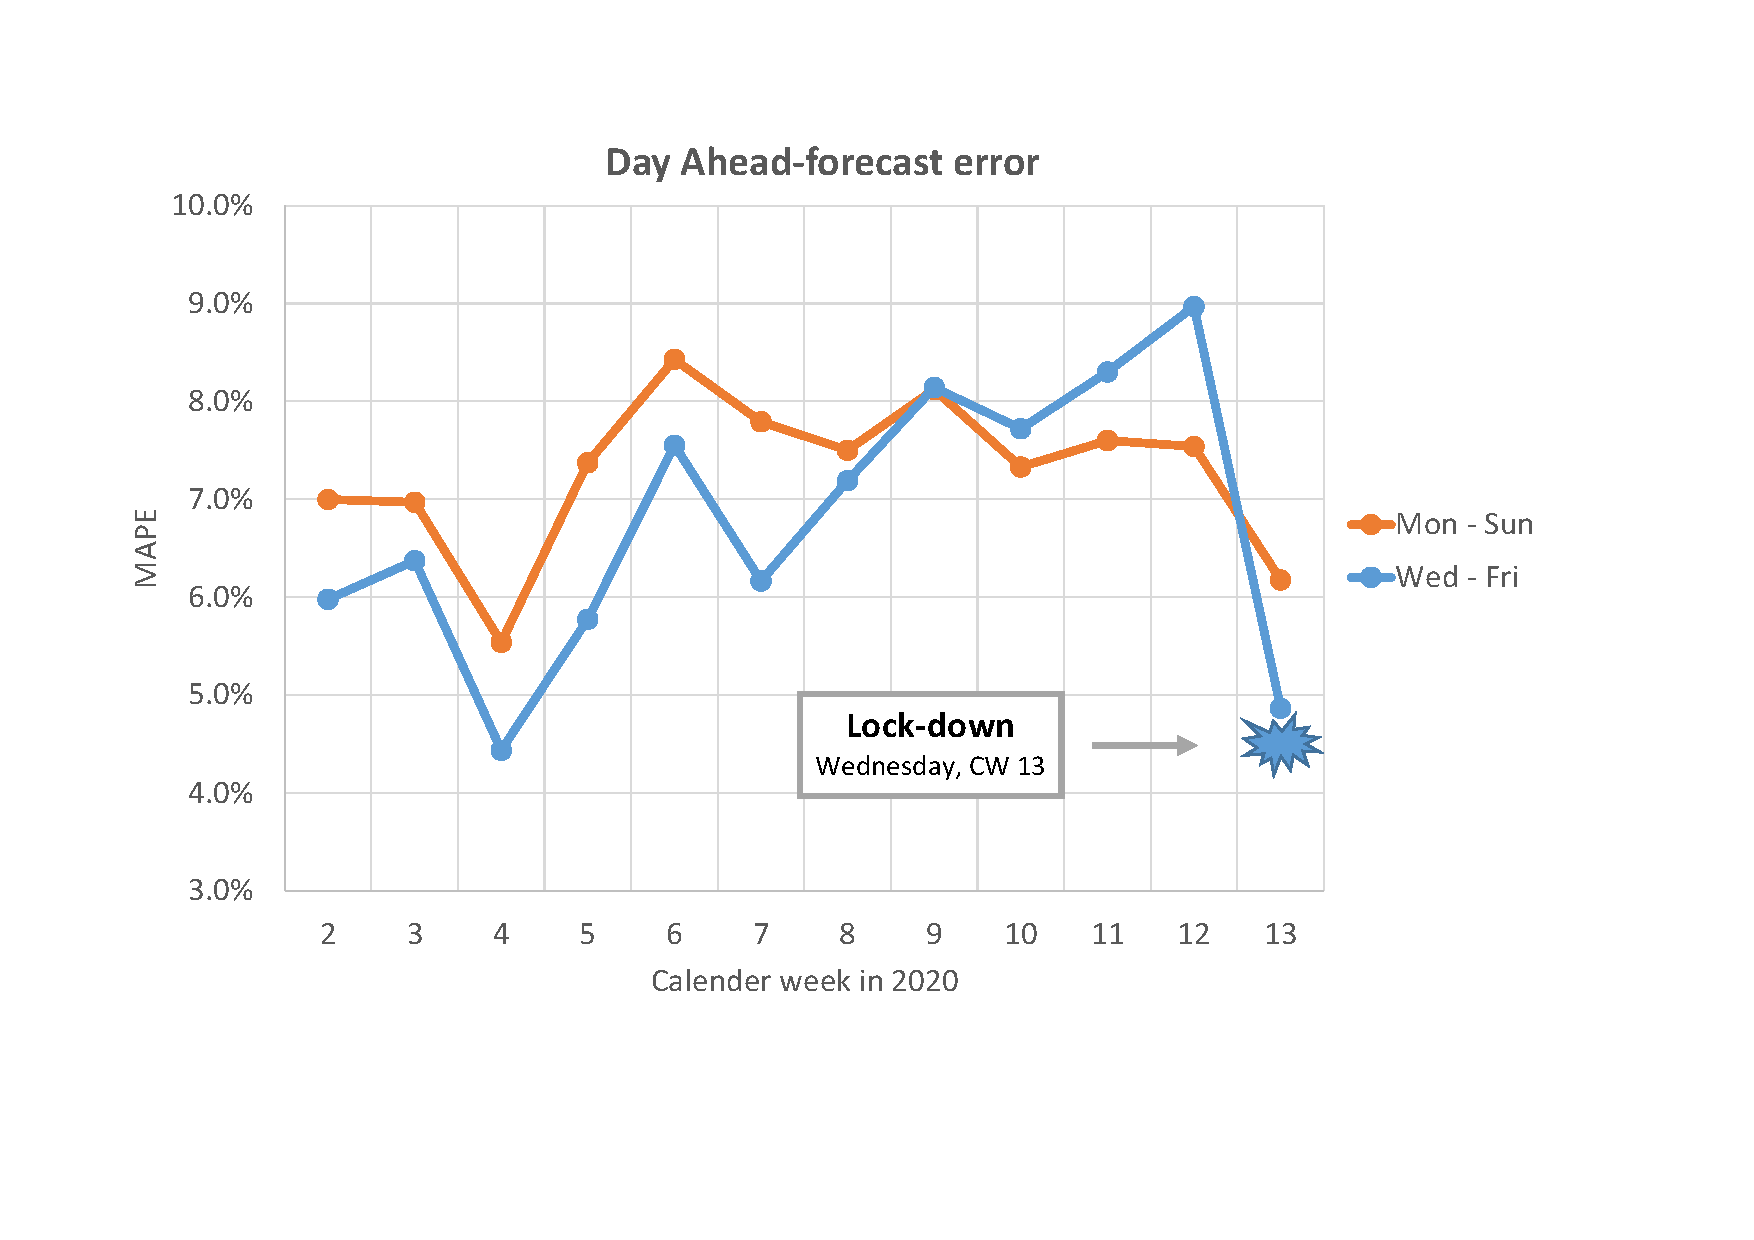
\includegraphics[trim={0cm 3cm 1cm 0.1cm},clip,width=16.5 cm]{Graphics/DAF-error.pdf}
%\caption{Weekly aggregated total Day-Ahead load forecast (DAF) error for the time frame from i) Monday to Sunday and ii) Wednesday to Sunday }
%\label{fig:DAF_forecast_error}
%\end{figure} 

%\begin{figure}[H]
%\centering
%\hspace{-25pt}
%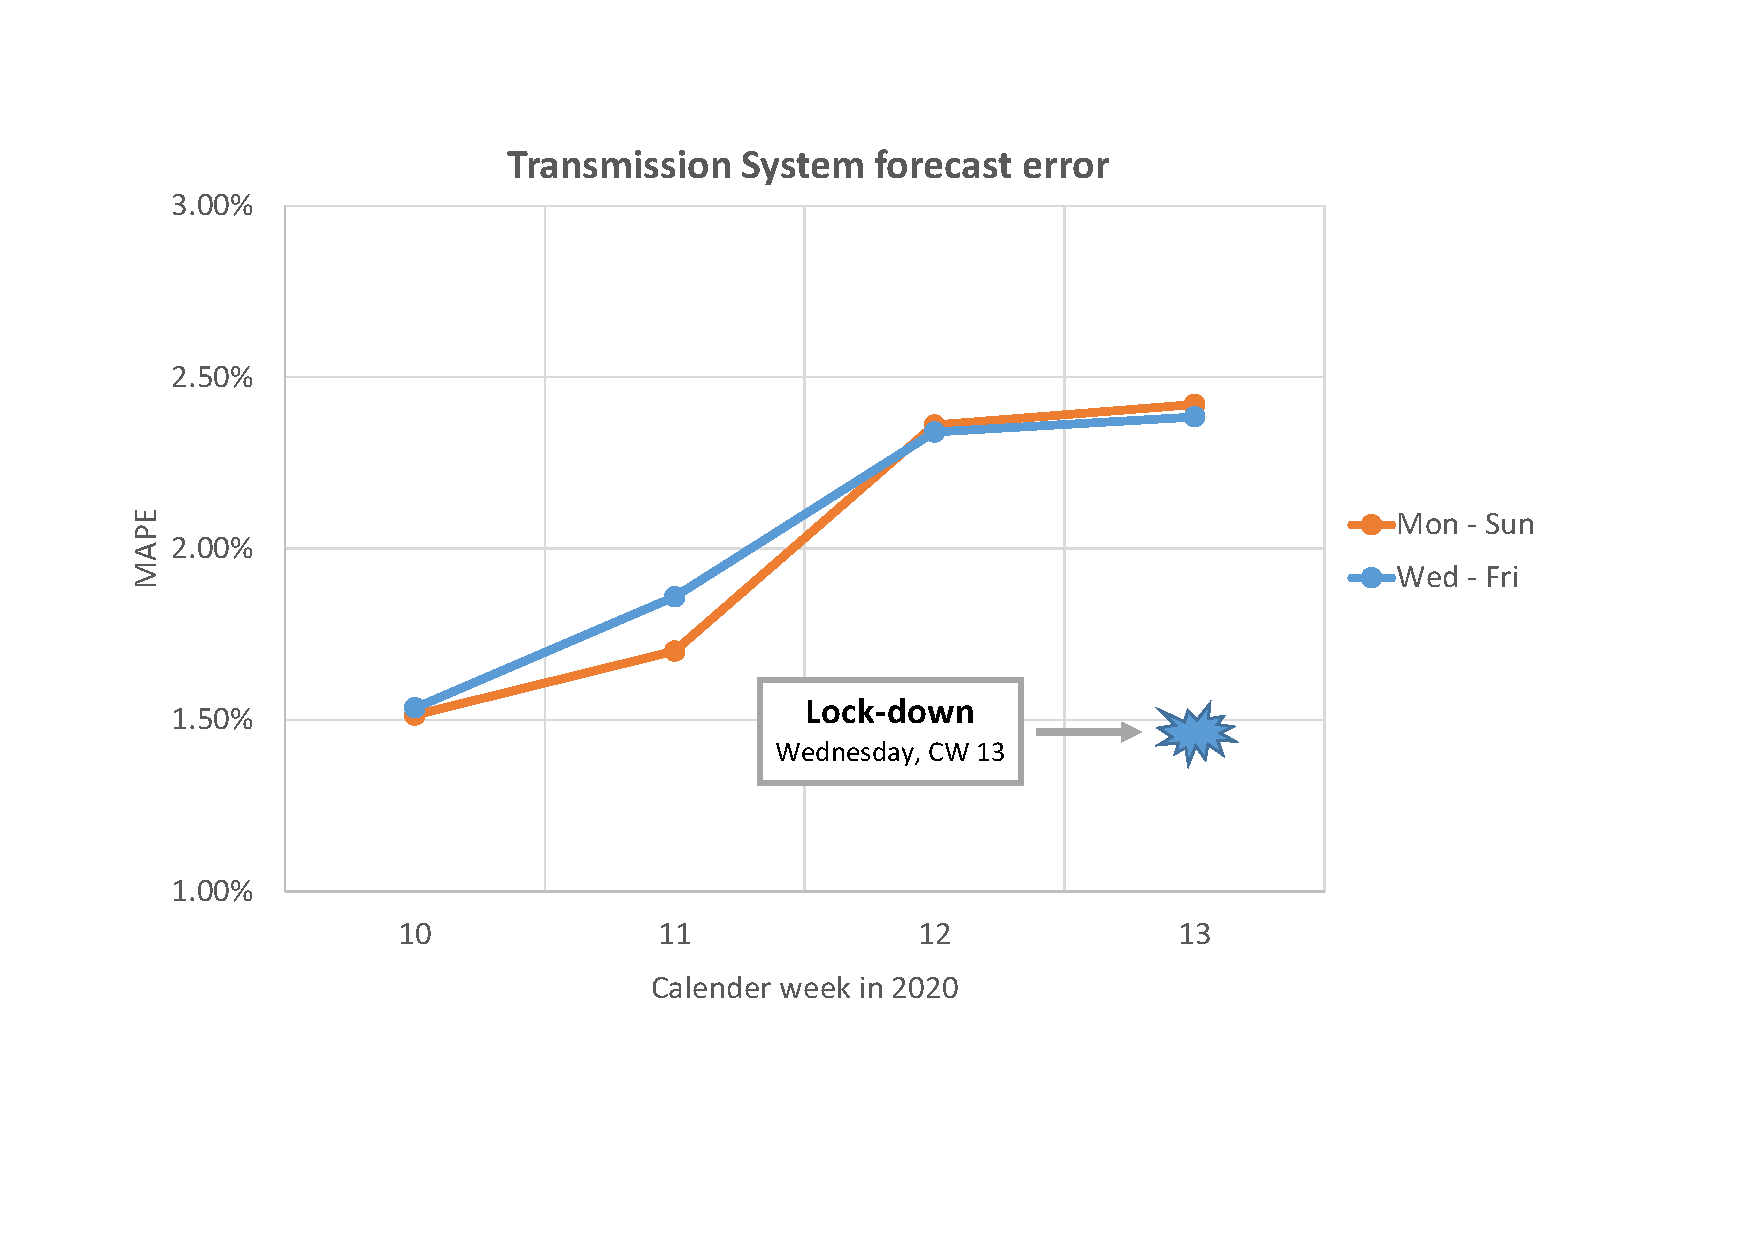
\includegraphics[trim={0cm 3cm 1cm 0.1cm},clip,width=16.5 cm]{Graphics/TSF-error.pdf}
%\caption{Weekly aggregated final transmission system load forecast (TSF) error for the time frame from i) Monday to Sunday and ii) Wednesday to Sunday }
%\label{fig:TSF_forecast_error}
%\end{figure} 


\begin{figure}[!tbp]
  \centering
  \subfloat[DAF error.]{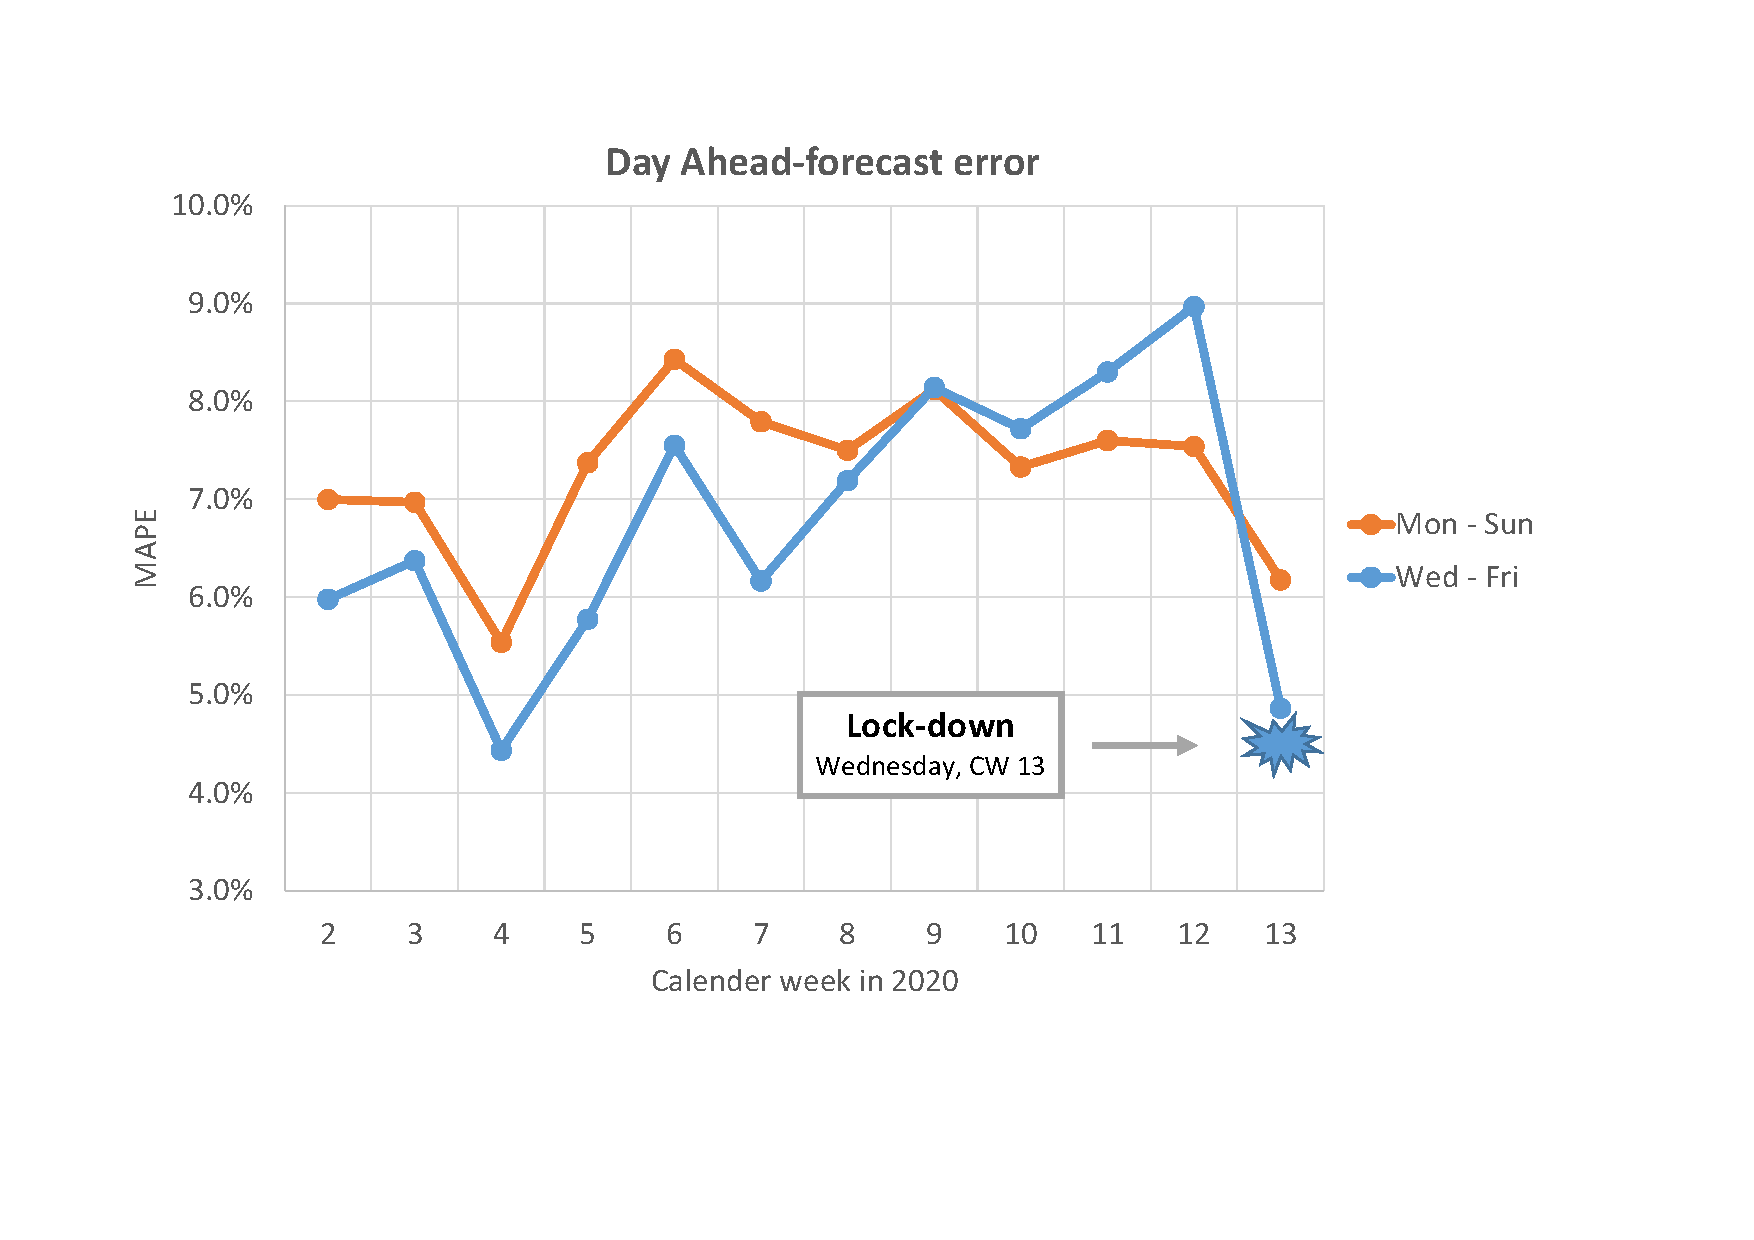
\includegraphics[trim={2cm 3cm 7cm 2cm},clip,width=0.45\textwidth]{Graphics/DAF-error.pdf}\label{fig:DAFerror}}
  \hfill
  \subfloat[TSF error.]{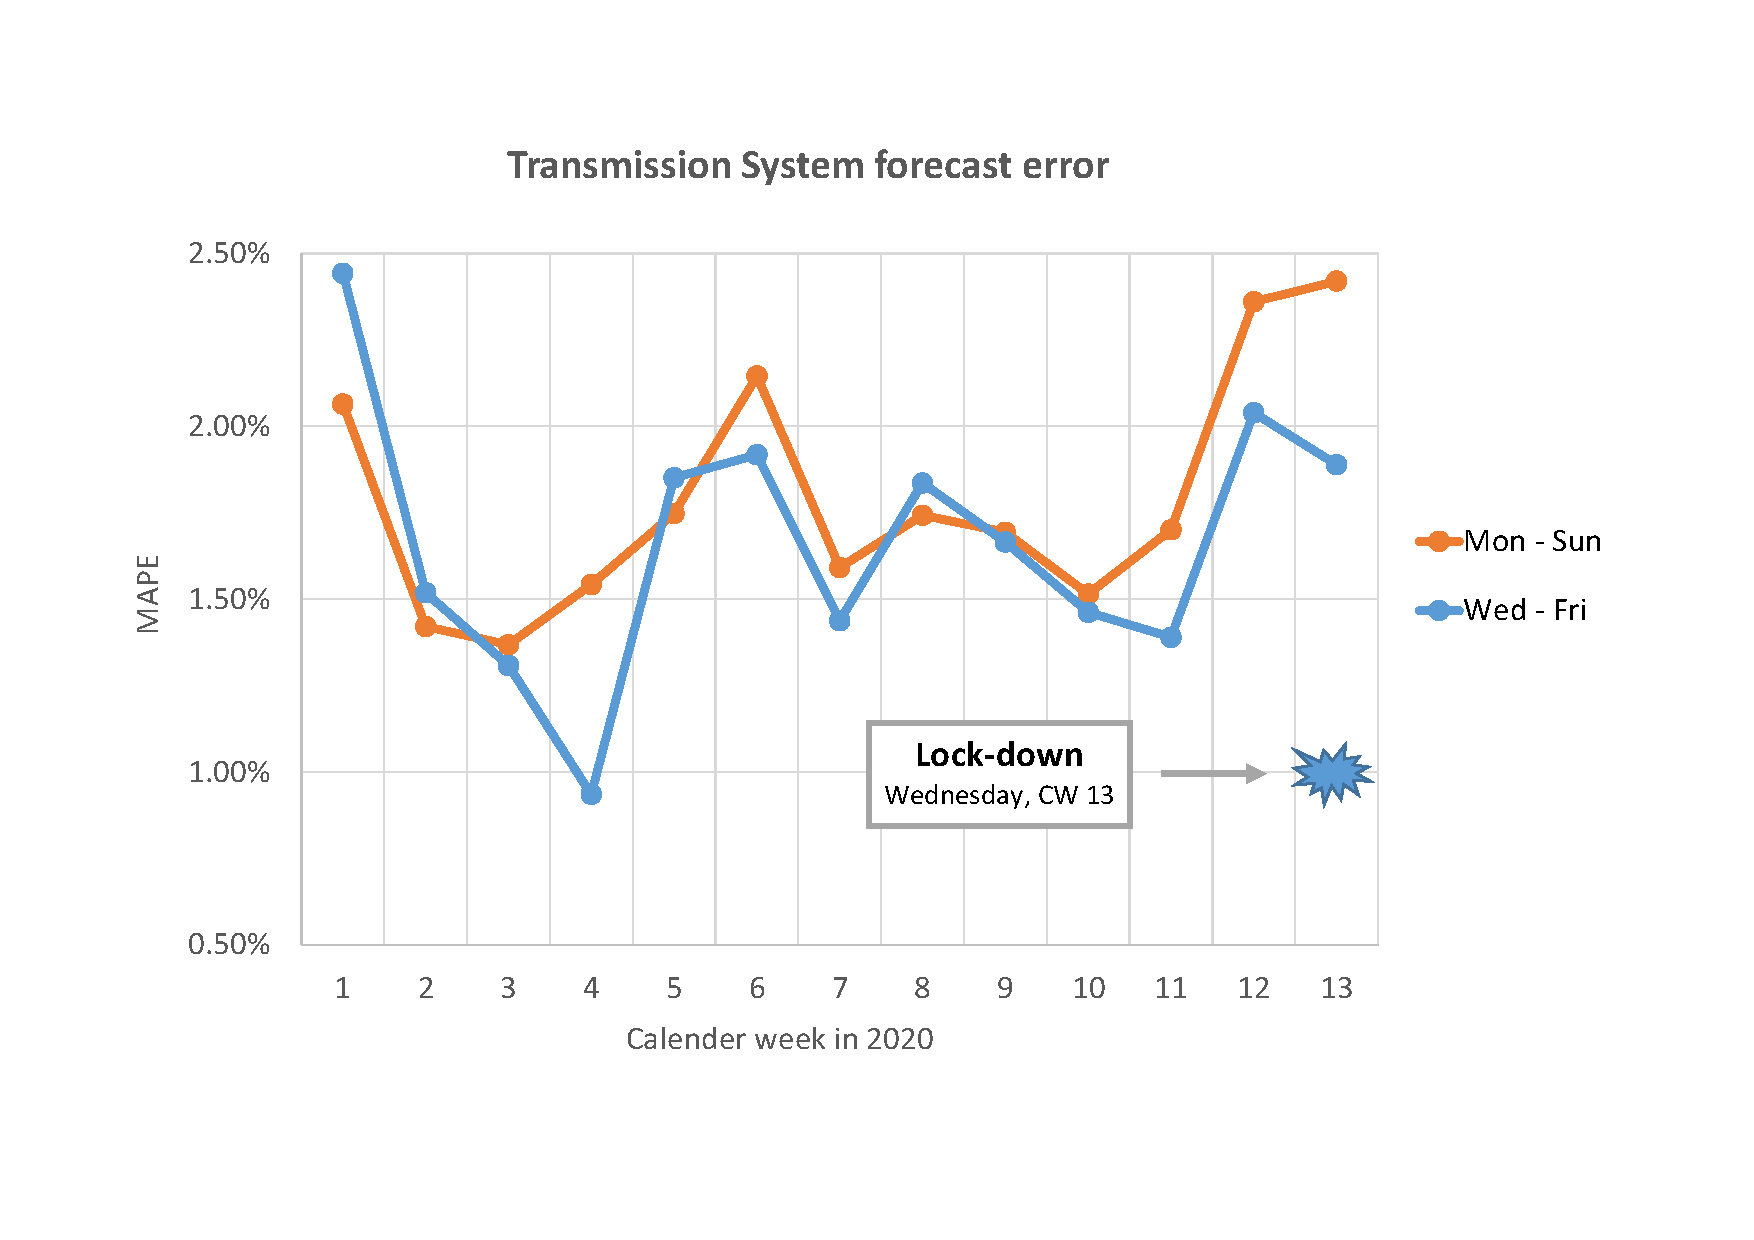
\includegraphics[trim={2cm 2cm 2.5cm 2cm},clip,width=0.53\textwidth]{Graphics/TSF-error-2020.pdf}
  \label{fig:TSFerror}}
  \caption{Weekly aggregated total Day-Ahead load forecast (DAF) and final transmission system load forecast (TSF) error, for the time frame from i) Monday to Sunday and ii) Wednesday to Friday. Note: The Wednesday to Friday frame was used to show the impact of the COVID-lockdown from the workday perspective.}
  \label{fig:DAFandTSFerror}
\end{figure}

%MAX: It seems I don´t have access to real DH data from ELEXON. Therefore, I take the DH data from ENTSO-E for the DH-forecast (long-term) and the ELEXON TSDF for short term forecast - 1h15min before SP.
%Max: It was recognized that both demand data are calculated with a different methodology. (ENTSO-E demand includes effect of all small and large embedded generation unit i.e. household PV or CHP &&& is adding it to the "demand"... Elexon NETSD data however doesn't take into account  net metering, which means that the net demand is smaller for Elexon as home PV is supplying some of the demand..). It of course complicate the comparison between both forecast, however, the general trend of better DH-forecast and worse short-term forecast is valid/interesting even if a "german-apple" is compared with a more delicious "scottish-one" - I would say we compare apple and banana in our case as they are still pretty based on similiar data.
% for short-term forecast would be more data from Desen, i.e. for complete year 2020, helpful
% On lower forecasterror. Additionally, the lower mid- and peak-load capacity during the day makes the load profile more steady.

%A previous note. The Day-Ahead load forecast turns out to be more precise due to new more steady load profile. The more steady load profile reduces the typically large load-change gradients, which are apparently responsible for uncertainty in the DA-load forecast.

%%%%%%%%%%%%%%%%%%%%%%%%%%%%%%%%%%%%%%%%%%%%%%%%%%%%%%%%%%%

\subsubsection{Deviations in  System Frequency}

The system frequency varies continuously and reflects the real-time discrepancies between system demand and total generation. Frequency increases when there is too much generation or too little demand on the system and vice versa.
Similar to other system operators, National Grid has a legal obligation to maintain system frequency within 49.5 and 50.5 Hertz \cite{ELEXON2020ELEXONBMRS}. This requires the system operators to accurately forecast demand and schedule generation accordingly whilst keeping a fast-response reserve or a demand action available for any unforeseen changes.
Nonetheless, the changes in frequency are also related to the system inertia. Introduction of most VRE generators such as solar panels and some types of storage such as batteries resulted in a decreased system inertia and consequently a less stable system frequency \cite{Ela2011OperatingReserves.}. Demand-side response (DSR) and other balancing services can be activated to ensure operation within the permitted range of frequency \cite{Nationalgrid2018BalancingStatement}. Currently, there is research assessing whether the wind and solar power plants could deploy synthetic inertia in order to compensate for this problem associated with VRE generation \cite{Hansen2014AnalysisTurbines, Zeni2013VirtualTurbines, Liu2017PV-basedSystem}. 

An abrupt change in the demand, like the one due to the lockdown, is expected to negatively affect the frequency. In this case, the frequency is expected to rise as the decrease in demand would result in a surplus of generation.
When analysed in its barest form, no significant discrepancies are observed for a pre and post COVID week. The mean and minimum and maximum frequency values also conclude an insignificant difference below 0.2 \% difference - see Table \ref{table:freq_table}. Despite the fact that both the minimum and maximum frequency values for the post-action week are higher than the pre-action week, the analysis is not sufficient to state a remarkable frequency variation due to the lock-down or perhaps more likely that it shows that the frequency was maintained well by the National Grid. 
% \begin{figure}[H]
% \centering
% \hspace{-25pt}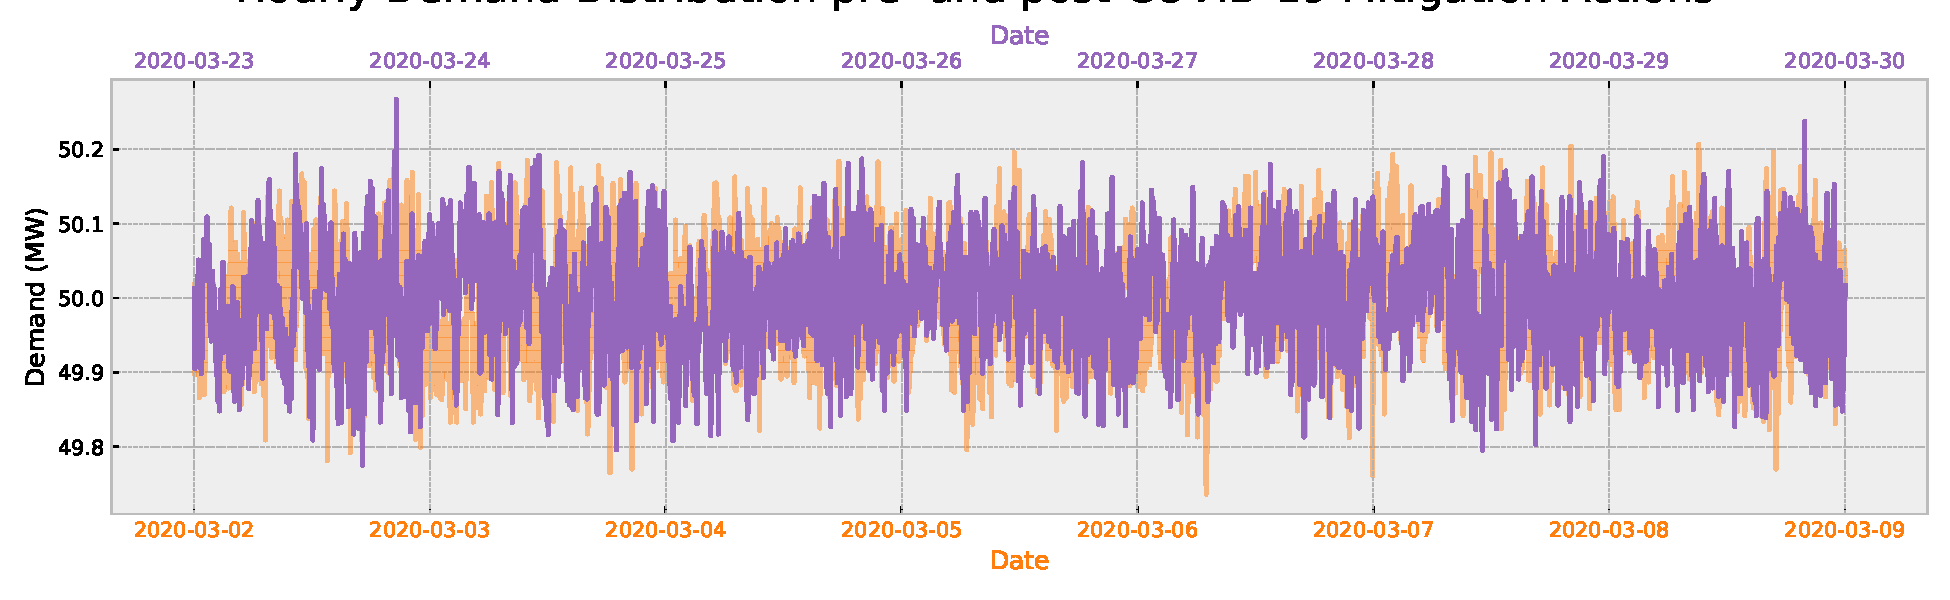
\includegraphics[trim={1cm 0cm 0 0.4cm}, clip, width=16.5 cm]{Graphics/Freq_pre_post_weekly.pdf}
% \caption{Comparison of pre and post-action system frequency where the y-axis is frequency in Hertz with 50 Hz being the nominal frequency.} \label{fig:freq_weekly}
% \end{figure}  

\begin{table}[H]
\caption{Comparison of descriptors to quantify the changes in the system frequency pre- and post-COVID-19 mitigation actions.}\label{table:freq_table}
\centering
%% \tablesize{} %% You can specify the fontsize here, e.g., \tablesize{\footnotesize}. If commented out \small will be used.
\begin{tabular}{cccc}
\toprule
\textbf{Data} & \textbf{Mean}	& \textbf{Min}	& \textbf{Max}\\
\midrule
Pre		& 49.998804			& 49.736000         & 50.207000\\
Post	& 49.998657			& 49.775000         &50.267000\\

\bottomrule
\end{tabular}
\end{table}

Hence, a normalised occurrence study is carried out to assess the distribution of system frequency in Figure \ref{fig:freq_hist}. The distribution for the post-action data has more defined peak around 50 Hz and its distribution width from 49.9 to 50.1 Hz is narrower. This suggests that the frequency was maintained within a stricter window than the pre-action week. The concentration of occurrence is below 50 Hz pre-lockdown whilst values above the nominal values are recorded more frequently after the lock-down (where the range of colours from yellow to dark blue in Figure \ref{fig:freq_hist} represents the highest to lowest occurrence respectively).
Hence, this displays a shift in the system frequency distribution, pointing out the increase in high frequency records. 

% When compared, the post-action frequency is narrower which suggests that more frequency corrections actions were taken.
% , however, indicates that the highest frequency occurrence changed from below 50 Hz to above 50 Hz at the post-COVID week. ???Not sure. Difference is not really clear as also x-axis changed. Any impacts???

\begin{figure}[H]
\centering

\hspace{-25pt}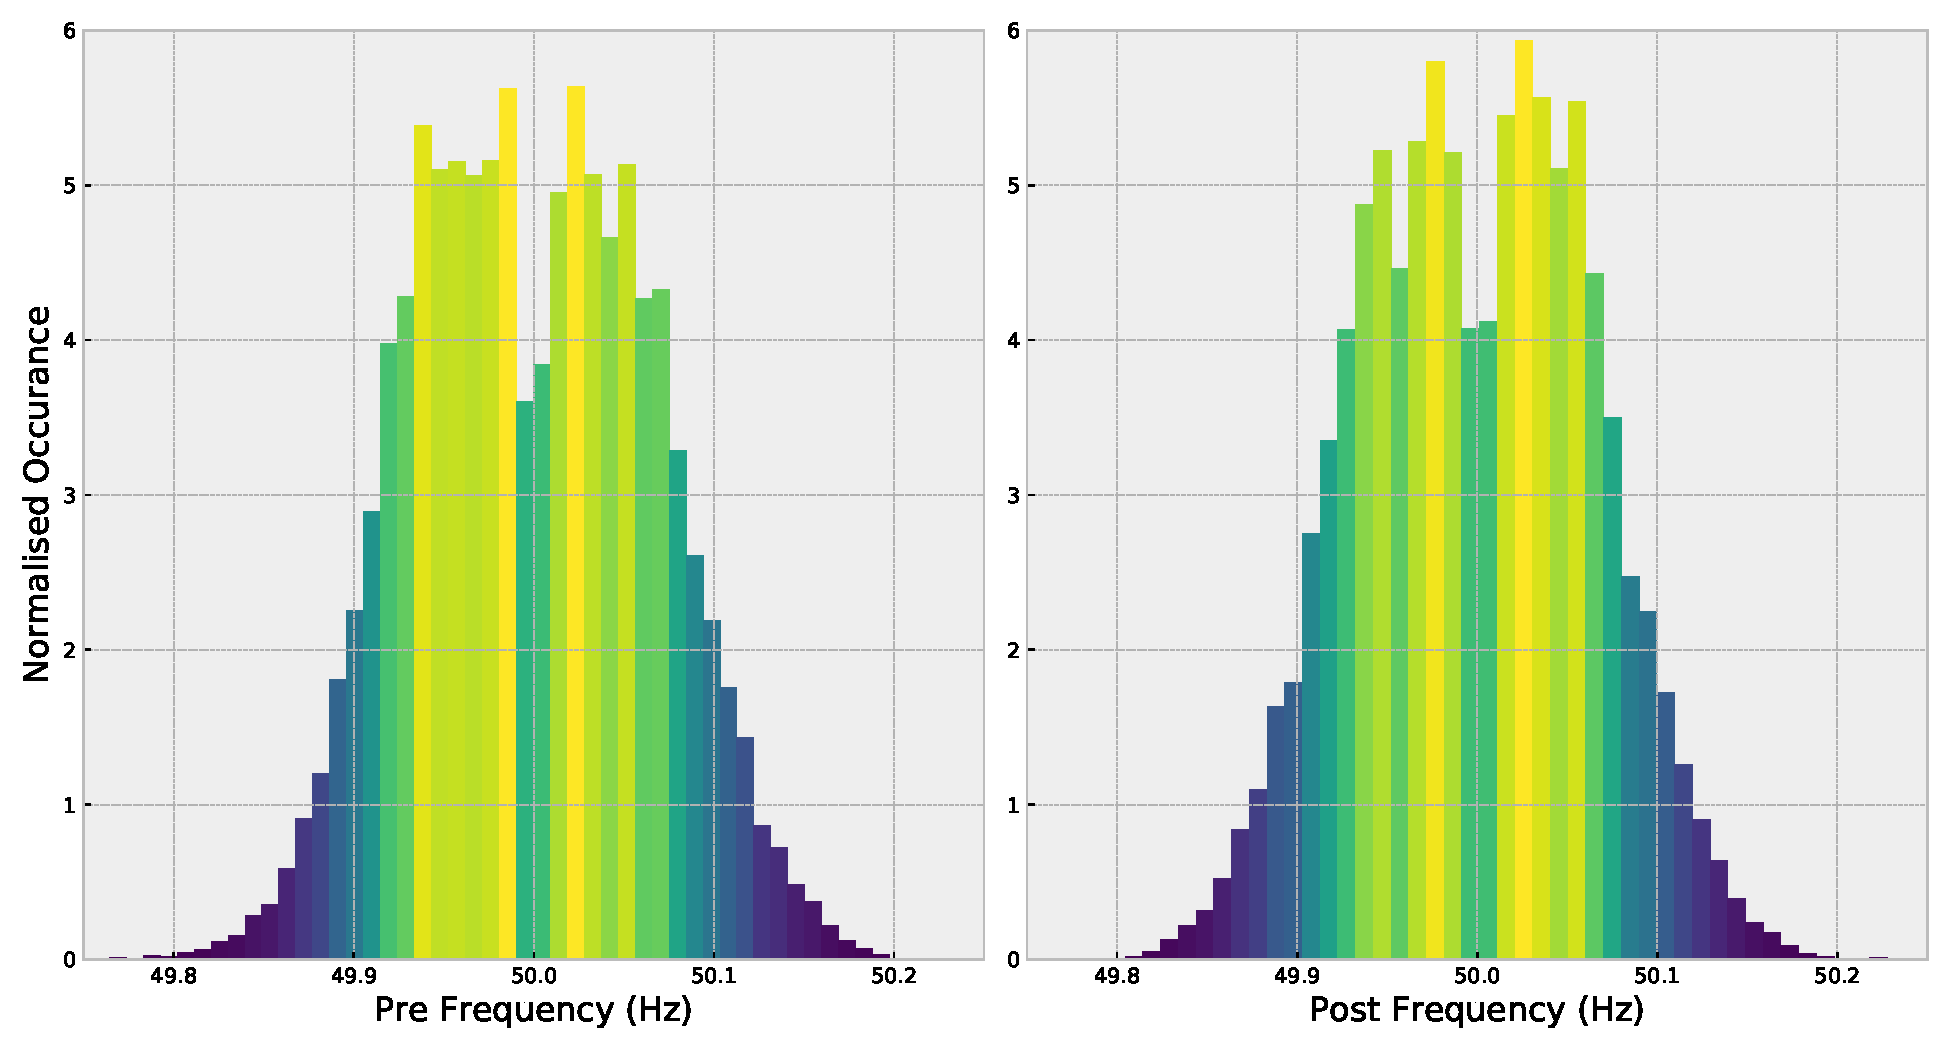
\includegraphics[ width=15 cm]{Graphics/NEW_Freq_hist_side_by_side.pdf}
\caption{Comparison of pre and post-action system frequency histograms} \label{fig:freq_hist}
\end{figure}  

One reason for this may be the decreased load profile, resulting a generation surplus, thus increasing the frequency - as discussed in Section \ref{section: Effect on demand profile}.
A peak-to-mean analysis is performed on both pre- and post-action data to compare the degree of variation. The frequency data is indexed by the time of the day. The most significant observation is regarding the high peak-to-mean ratio calculated for 8 p.m. for the post-COVID-19 week. This maybe because of the unforeseen changes in the shape of the consumption profile - this is discussed in Section \ref{section: Effect on demand profile}.
% 1. Peak-to-Mean ratio increased during lunch
% 2. Peak-to-Mean ration increased during "prime time"
% 3. Peak-to-Mean ratio decreased at night
% 4. Peak-to-Mean ration decreased in the morning and afternoon
% ????? INTERPRETATION PARTLY UNCLEAR ????? Prime time indicates more family TV times at 8pm (10 million TV´s equals demand of roughly 7GW)


\begin{figure}[H]
\centering
\hspace{-25pt}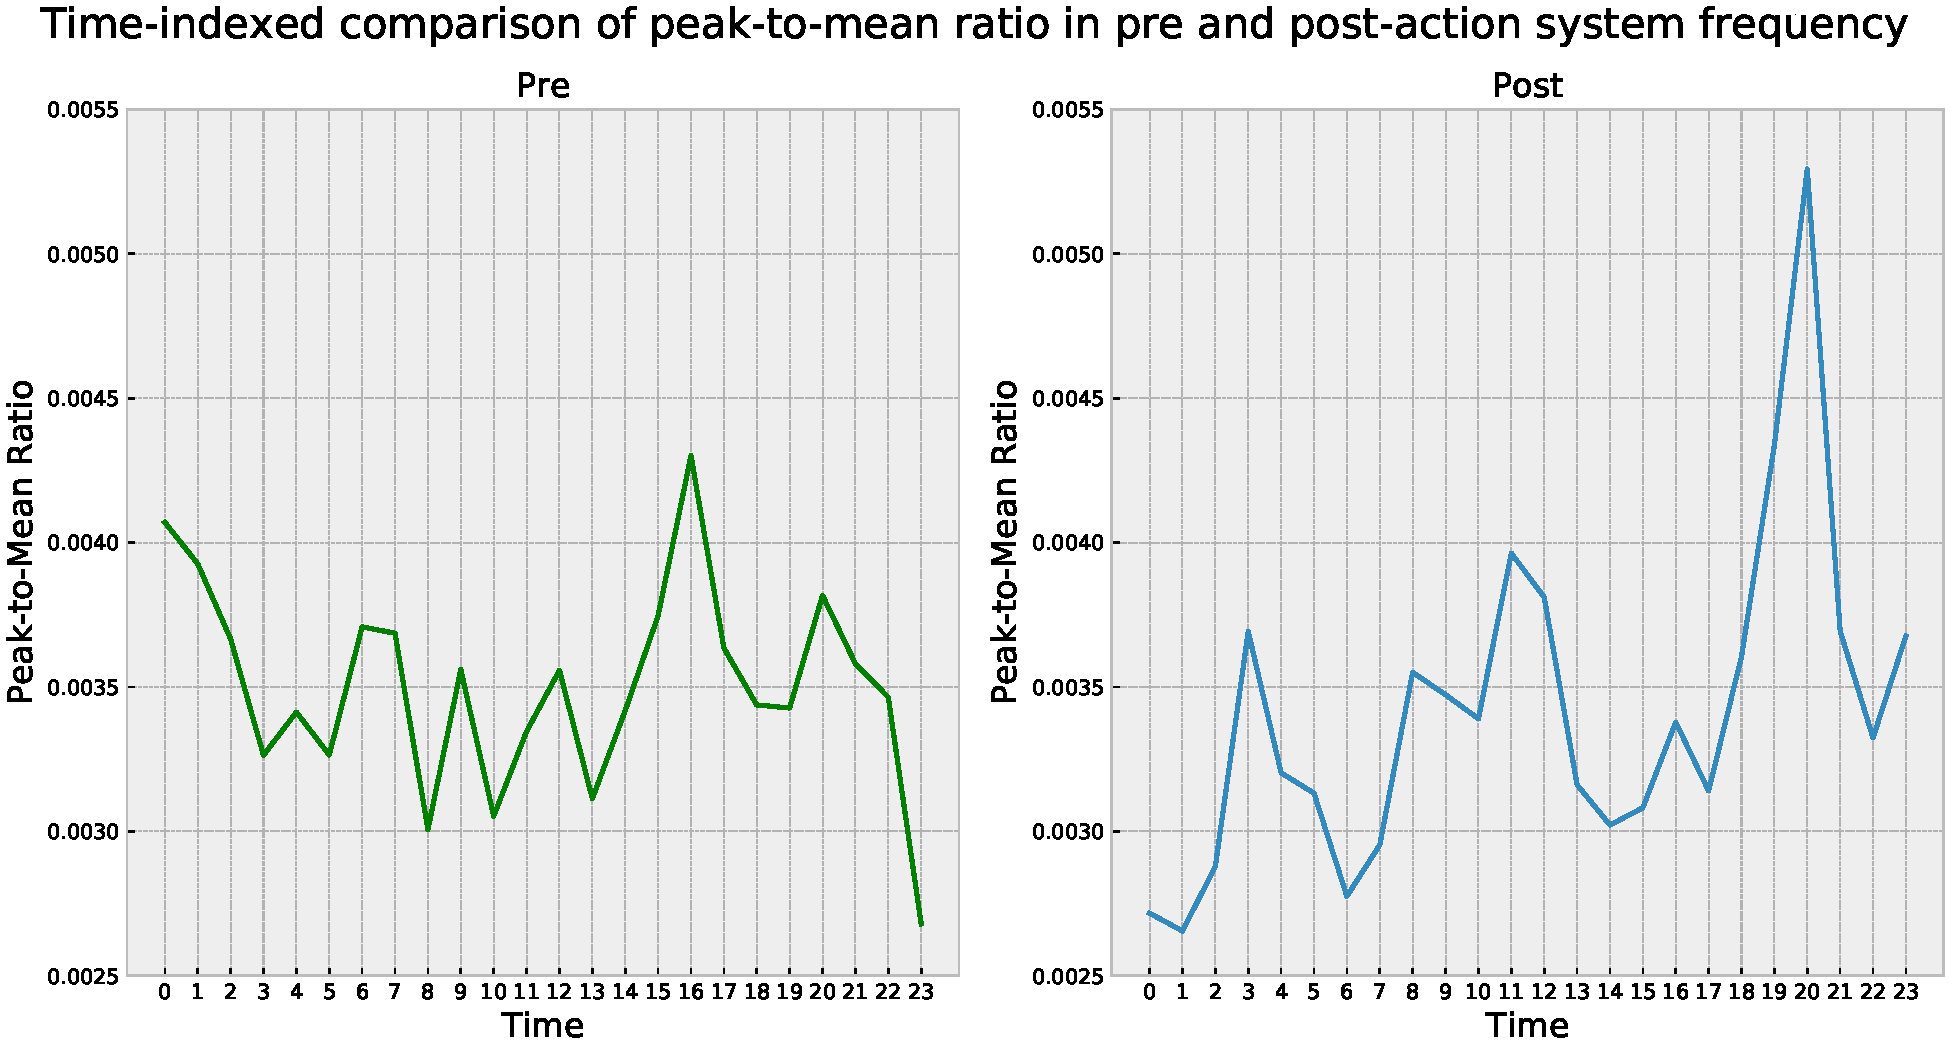
\includegraphics[width=14 cm]{Graphics/NEW_Freq_PtM_comp.pdf}
\caption{Comparison of Pre and Post-action System Frequency Peak-to-Mean Ratios} \label{fig:freq_PtM}
\end{figure}  

% 1. Frequency is varying/changing/jumping less on average. Maybe due to the lower peak to base-load ratio ("smoother profile").

% \begin{figure}[H]
% \centering
% \hspace{-25pt}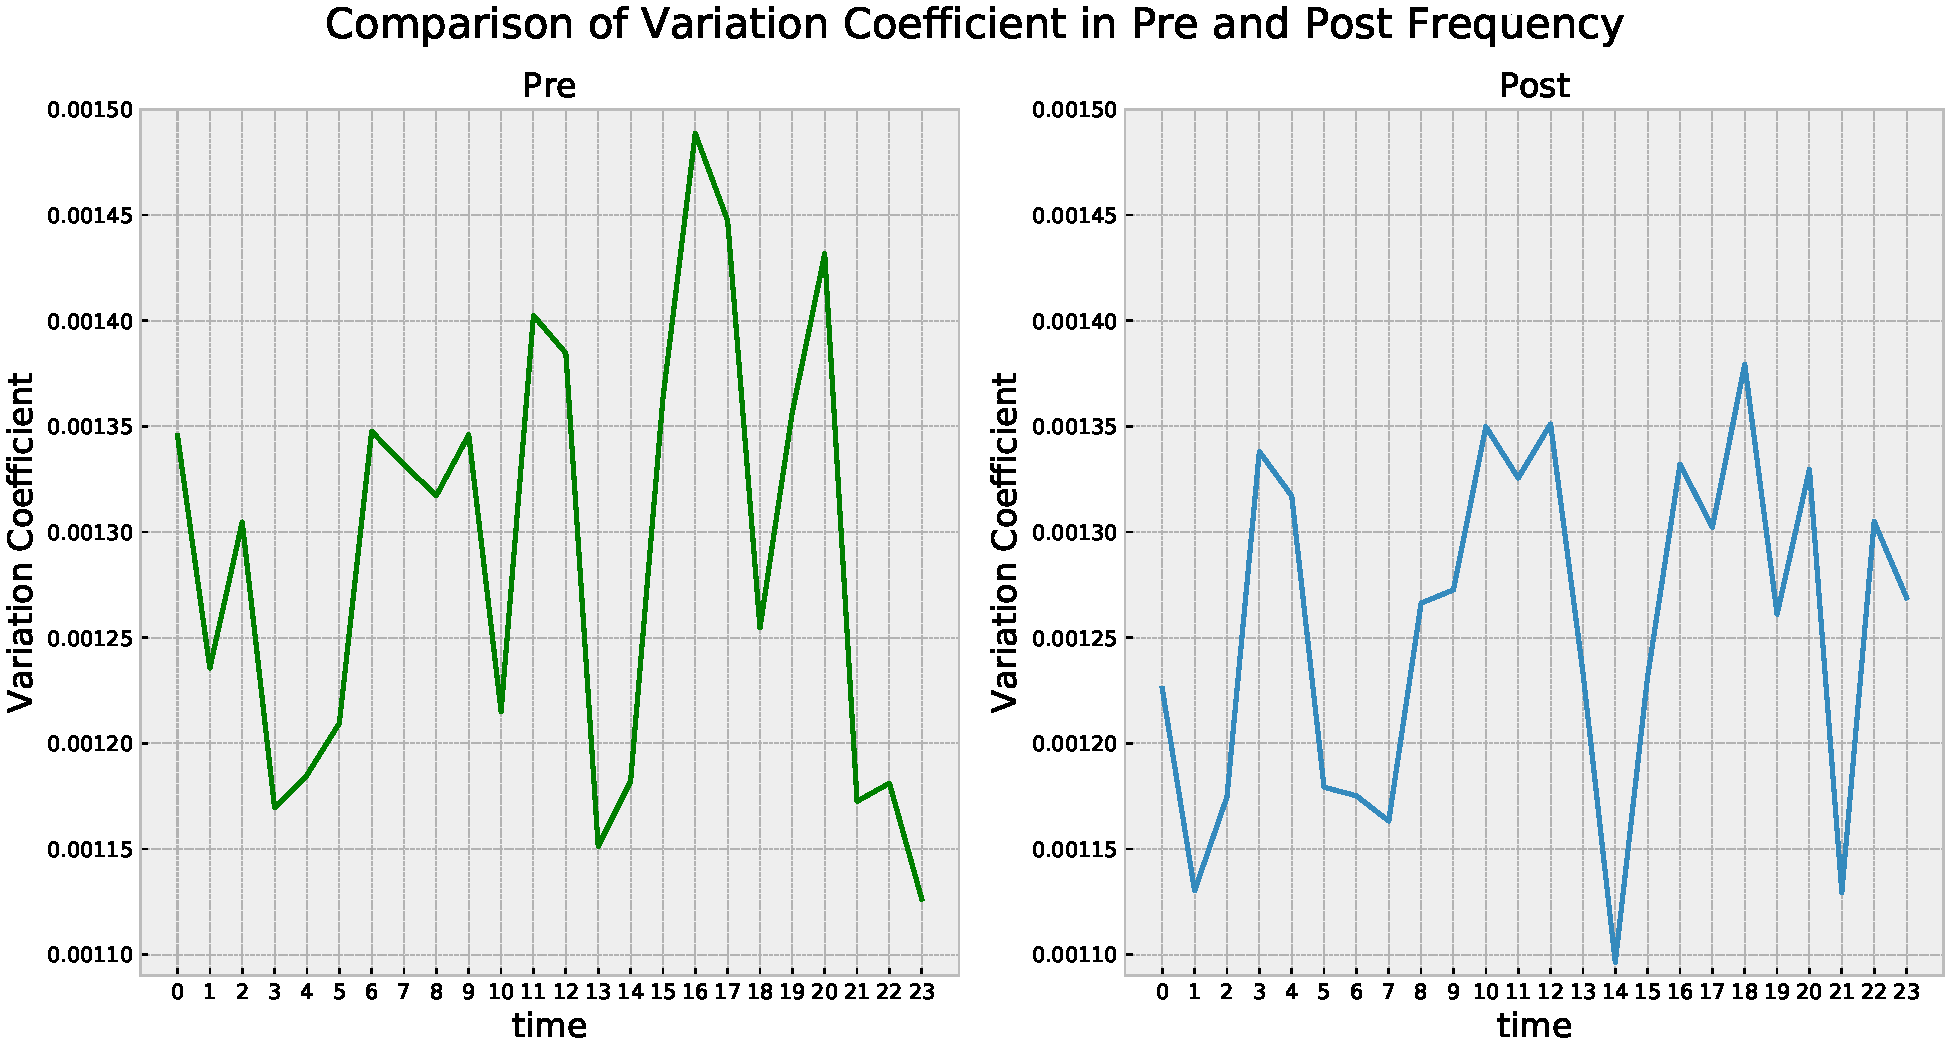
\includegraphics[width=16.5 cm]{Graphics/FFreq_VarCoeff_comp_2.pdf}
% \caption{Comparison of Pre and Post-action System Frequency Variation Coefficient} \label{fig:freq_hist}
% \end{figure}  

% Moreover, the on average higher share of VRE generation assets (see \ref{sec:Generation portfolio}) makes the power system more prone for rapid frequency changes \cite{Ela2011OperatingReserves.}. The reason behind this is the change of inertia in the power system. Inertia is provided by conventional synchronous generators, such as in coal, gas, biomass or hydro plants representing spinning masses that store kinetic energy. When for instance, the frequency drops, the rotation of the synchronous generators reduces, providing extra kinetic energy which lowers the supply-demand mismatch or frequency drop. Therefore, a power system with lower inertia, such in case when the share of VRE is high, lead to higher frequency changes in short-term, before any balancing reserve helps out to clear the imbalance. 




%Impact of changing generation portfolio on frequency.
%importance of inertia
%generation portofolio and impact intertia
% Sum What the change in inertia will do to the frequency?

%%%%%%%%%%%%%%%%%%%%%%%%%%%%%%%%%%%%%%%%%%%%%%%%%%%%%%%%%%%%%%%%%%%%%%%%%%%%%%%%%%%%%%

\subsubsection{Imbalance Volume}\label{section:ImbalanceVolume}

An imbalance is prevalent in the power system when supply does not match demand. If the imbalance is not tackled, it could lead to an unstable frequency and finally black-outs. It is therefore the System Operators (SO) responsibility to keep the balance in the system \cite{ELEXON2020ELEXONBMRS}. All accepted balancing measures in a settlement period are given by the net imbalance volume (NIV), which represents the total sum of positive and negative system management and energy balancing measure in the settlement period \cite{ELEXON2020ELEXONBMRS}. In a perfect market the power plants are scheduled at gate-closure that demand equals supply at any settlement period to ensure a NIV close to zero. However, the energy balance in a settlement period is usually not met, since \cite{ELEXON2019GuidanceBritain}:
\begin{itemize}
    \item Demand prediction errors by suppliers
    \item Generation prediction errors by generators (i.e. not able to tightly control the operation of intermittent units)
    \item Problems in transmission lines
    \item Balance must exist at every instant, but market trades in half-hour settlement periods 
\end{itemize}

In section \ref{DemandForecastError}, it was recognised the short-length load forecast accuracy decreased slightly. The consequences of this poorer short-length forecast are amplified in the NIV and cause the NIV to grow significantly compared to all other calendar weeks in 2020, see Figure \ref{fig:ImbalanceVolume_over_2020}. Which means whatever changed at the lock-down week, increased the amount and volume of balancing measures in the power system.


\begin{figure}[H]
\centering
\hspace{-25pt}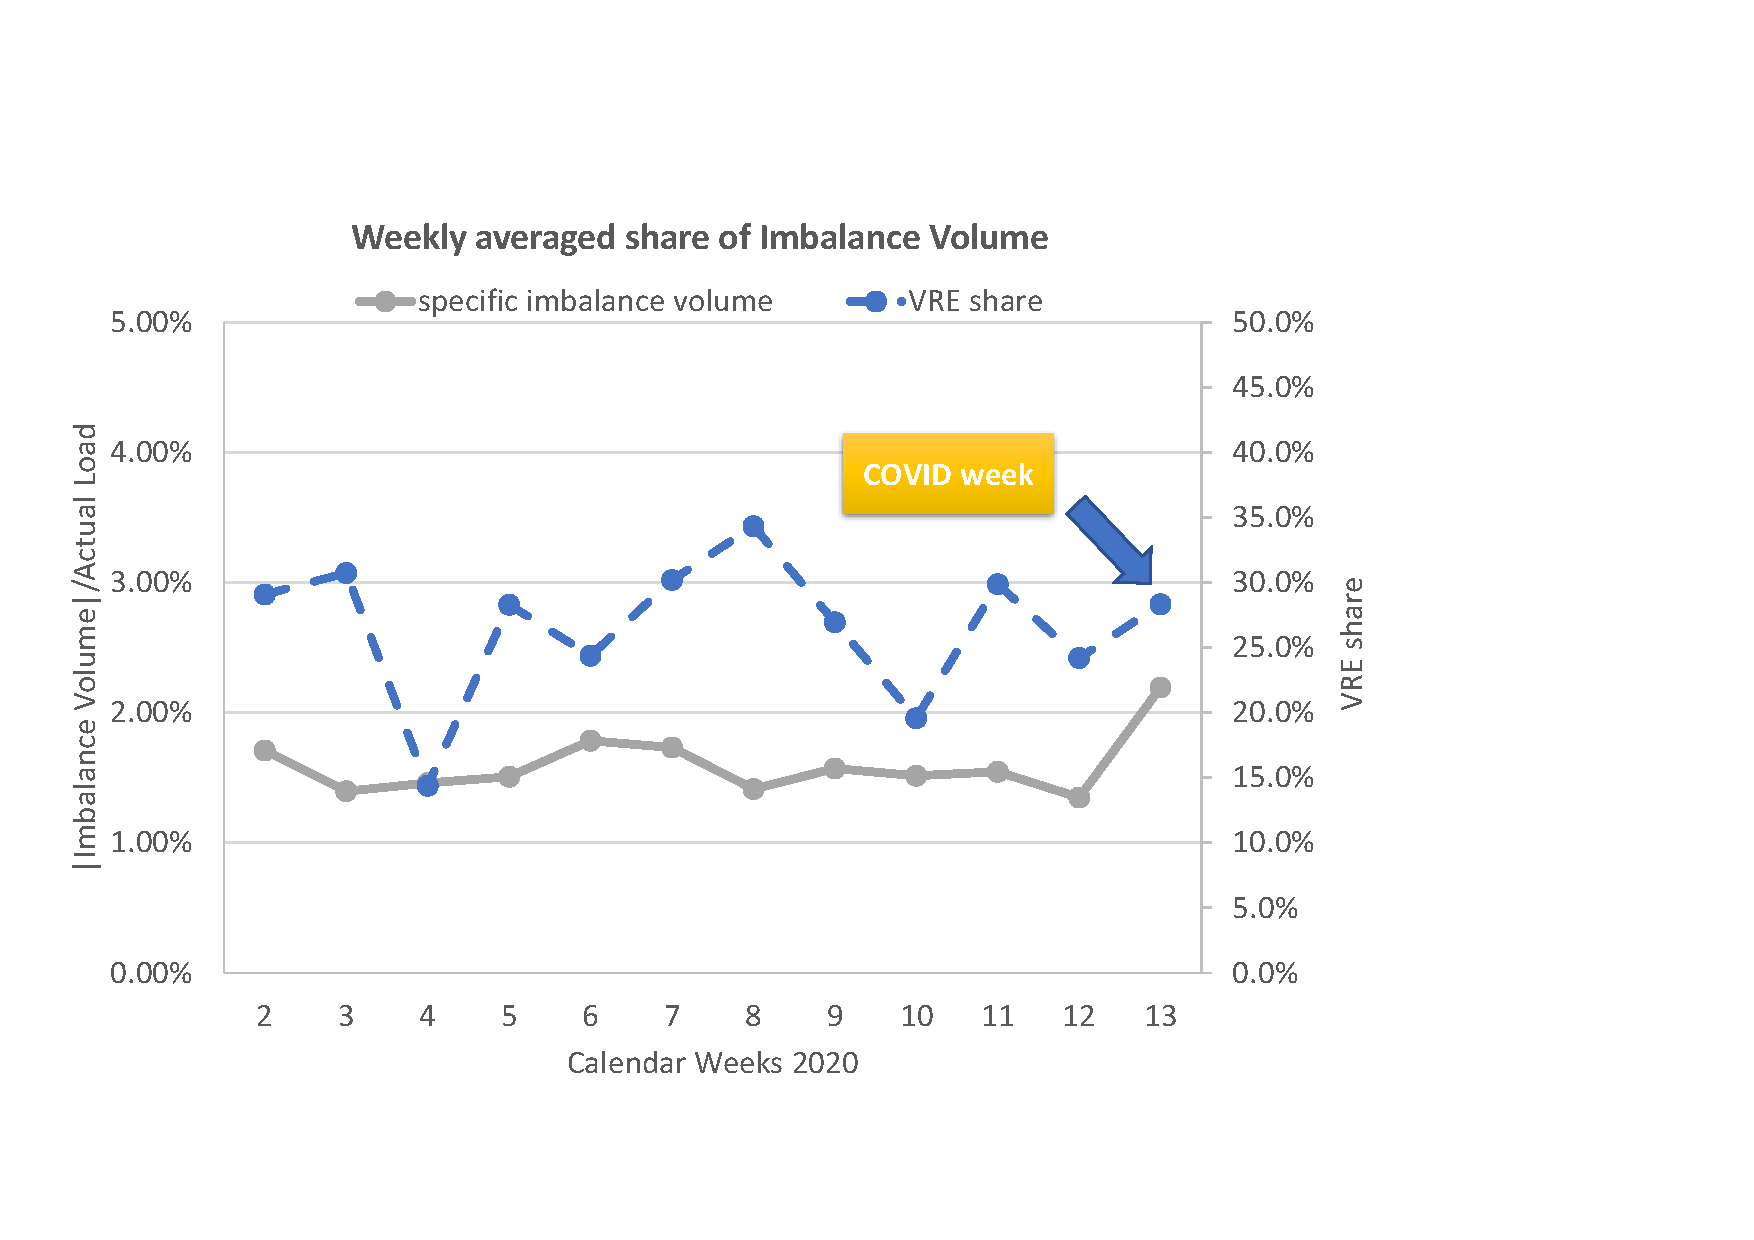
\includegraphics[trim={0cm 2cm 6.5cm 3.5cm},clip,width=0.7\textwidth]{Graphics/Illustration-Imbalance-2020.pdf}
\caption{The weekly average share of imbalance volume factorised by the actual total load. Data from ENTSO-E \protect\cite{ENTSO-E2020ENTSO-EPlatform}}
\label{fig:ImbalanceVolume_over_2020}
\end{figure} 

The higher share of VRE seems to be the main driver for the increasing imbalance in the power system after the lock-down. In Figure \ref{fig:ImbalanceVolume-daily}, the imbalance volume was weighted to the actual total system demand for a pre- and post-COVID week. On the secondary axes is VRE share plotted. Remarkable is the correlation between weighted imbalance volume and the VRE share after the lock-down. The correlation might be not a permanent condition in future. When analysing data from January to March, a correlation between VRE share and imbalance volume was discovered roughly 20\% of the time, though, at approximately 80\% of the time there is no clear correlation visible. Nevertheless, a clear correlation between VRE share and imbalance volume is observed after the lock-down, which indicates that the increasing VRE share is the main driver for the higher imbalance volume. The reason for that cannot be precisely untangled as four things can cause an imbalance: generation and demand prediction errors, network constraints, and the balance need at every instance. 

\begin{figure}[H]
\centering
\hspace{-25pt}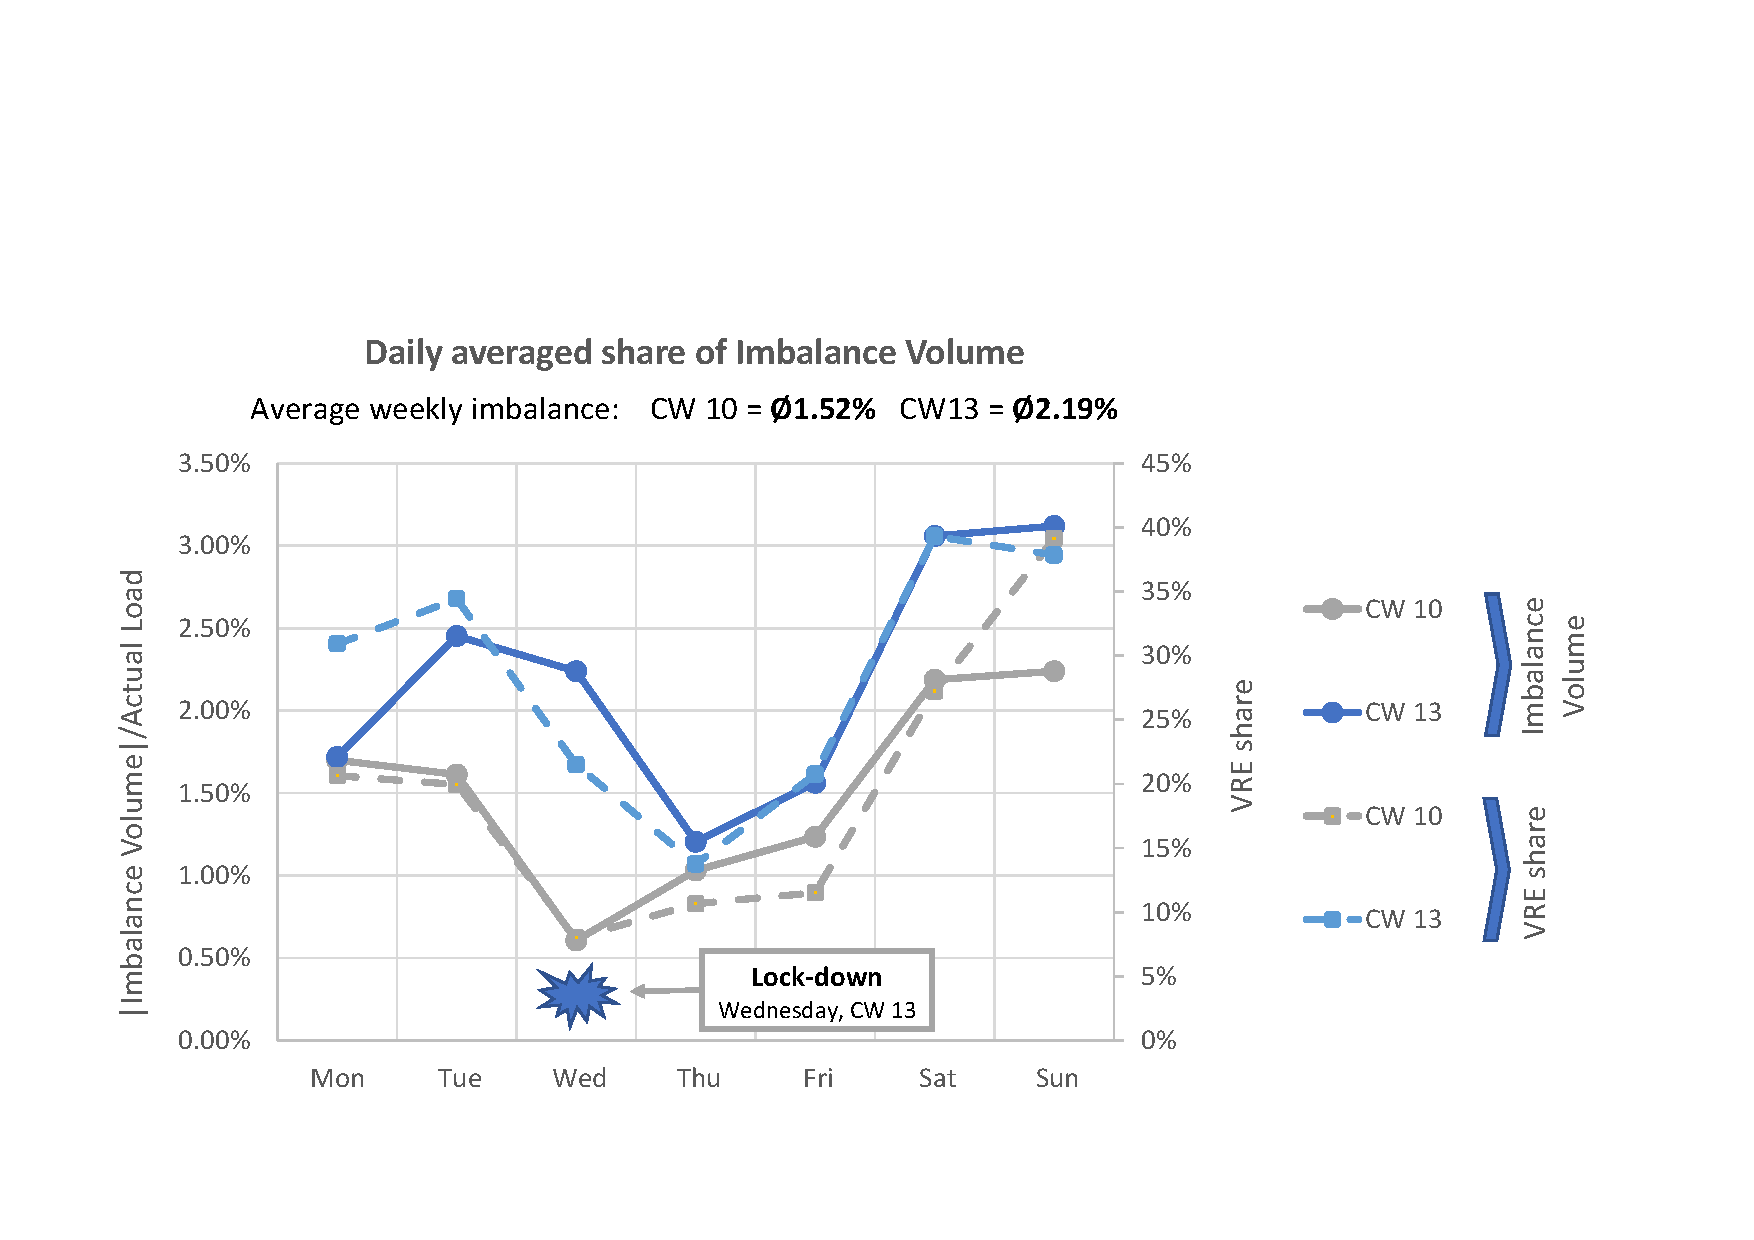
\includegraphics[trim={0cm 2cm 2.5cm 4cm},clip,width=1\textwidth]{Graphics/Illustration-Imbalance-2weeks.pdf}
\caption{Daily average share of imbalance volume and share of VRE for one pre- and post-COVID week, 02-09 March and 22-28 March, respectively. All data available at \protect\cite{ELEXON2020ELEXONBMRS}.}\label{fig:ImbalanceVolume-daily}
\end{figure} 

The effect of higher VRE shares explains the slightly poorer performance of the short-length load forecast TSF, as embedded VRE, which consists of 13 GW solar and 6 GW wind capacity in 2018,  cause load forecast errors \cite{NationalgridESO2018QuarterlyMarch18, NationalGridESO2019EnergyRoadmap}. Contrary, the Day-Ahead load forecast improved, so there might be a trade-off between the benefit of smoother load-profiles and the bad influence of high VRE shares on forecast errors. In summary, it seems that depending on the forecast length, the COVID situation causes improved or worse load forecast performance, see Figure \ref{fig:Illustrative-forecast-summary}. Shorter load forecast-length drop in performance, while longer forecast-length increase in performance.

\begin{figure}[H]
\centering
\hspace{-25pt}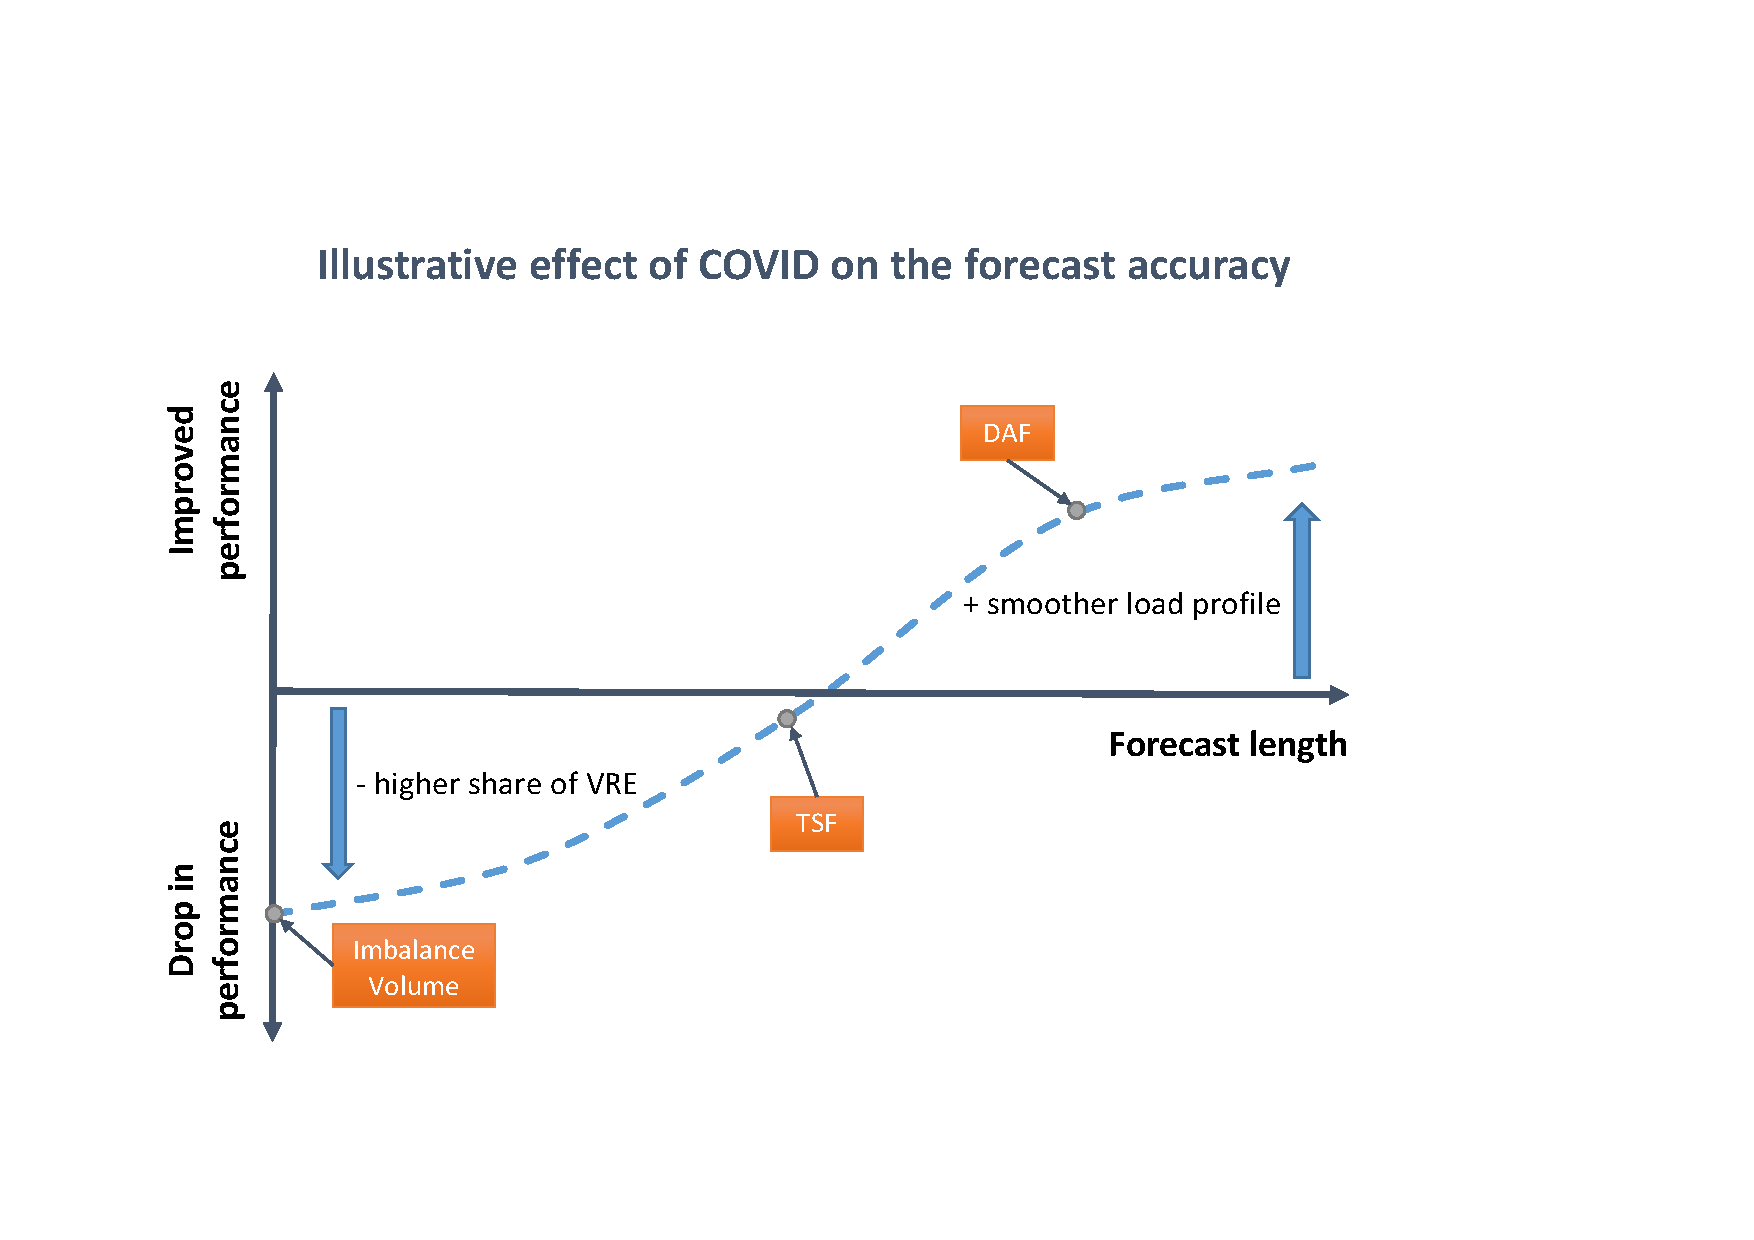
\includegraphics[trim={-1cm 3cm 3cm 3cm},clip,width=1\textwidth]{Graphics/Illustrative-forecast-summary.pdf}
\caption{Illustrative effect of COVID on the forecast accuracy compared to pre-COVID weeks. TSF and DAF indicate the transmission system forecast and total Day-Ahead forecast, respectively, as described in section \ref{DemandForecastError}.}\label{fig:Illustrative-forecast-summary}
\end{figure} 

%%%%%%%%%%%%%%%%%%%%%%%%%%%%%%%%%%%%%%%%%%%%%%%%%%%%%%%%%%%%%%%%%%%%
\subsubsection{LOLP}\label{section:LOLP_DRM}

Loss of load probability (LOLP) is an indicator for system reliability measured by the system operator for each settlement period \cite{ELEXON2019GuidanceBritain}. For instance, when National Grid predicts higher probability of loss of load, the balancing mechanism is willing to pay higher prices for balancing at the time of reserve scarcity. The methodology to calculate the LOLP can be found in \cite{Elexon2019LossStatement}. The higher prices at high LOLP levels are also known as reserve scarcity prices, which are the product of LOLP and the value of lost load (VoLL). Whereby, the VoLL is determined through the assessment of how much value consumers on average attribute to the security of supply - currently set on £6000/MWh \cite{ELEXON2019GuidanceBritain}. 

\begin{equation}\label{eq:reservescarc}
Reserve Scarcity Price = Lost of Load Probability \times Value of Lost Load
\end{equation}
Due to the abrupt changes in the demand profile and eventually the inflexibility of the available generation, National Grid predicted a higher LOLP during the evening of the 25th of March which is the first official day of lock-down (see Figure \ref{fig:LOLP_25_03}). Despite the fact that it was predicted 12 hours in advance, the 1 hour ahead LOLP forecast is 4.5 times higher. This implies that there was a reserve scarcity and/or that the grid was under stress.

\begin{figure}[H]\centering
\hspace{-25pt}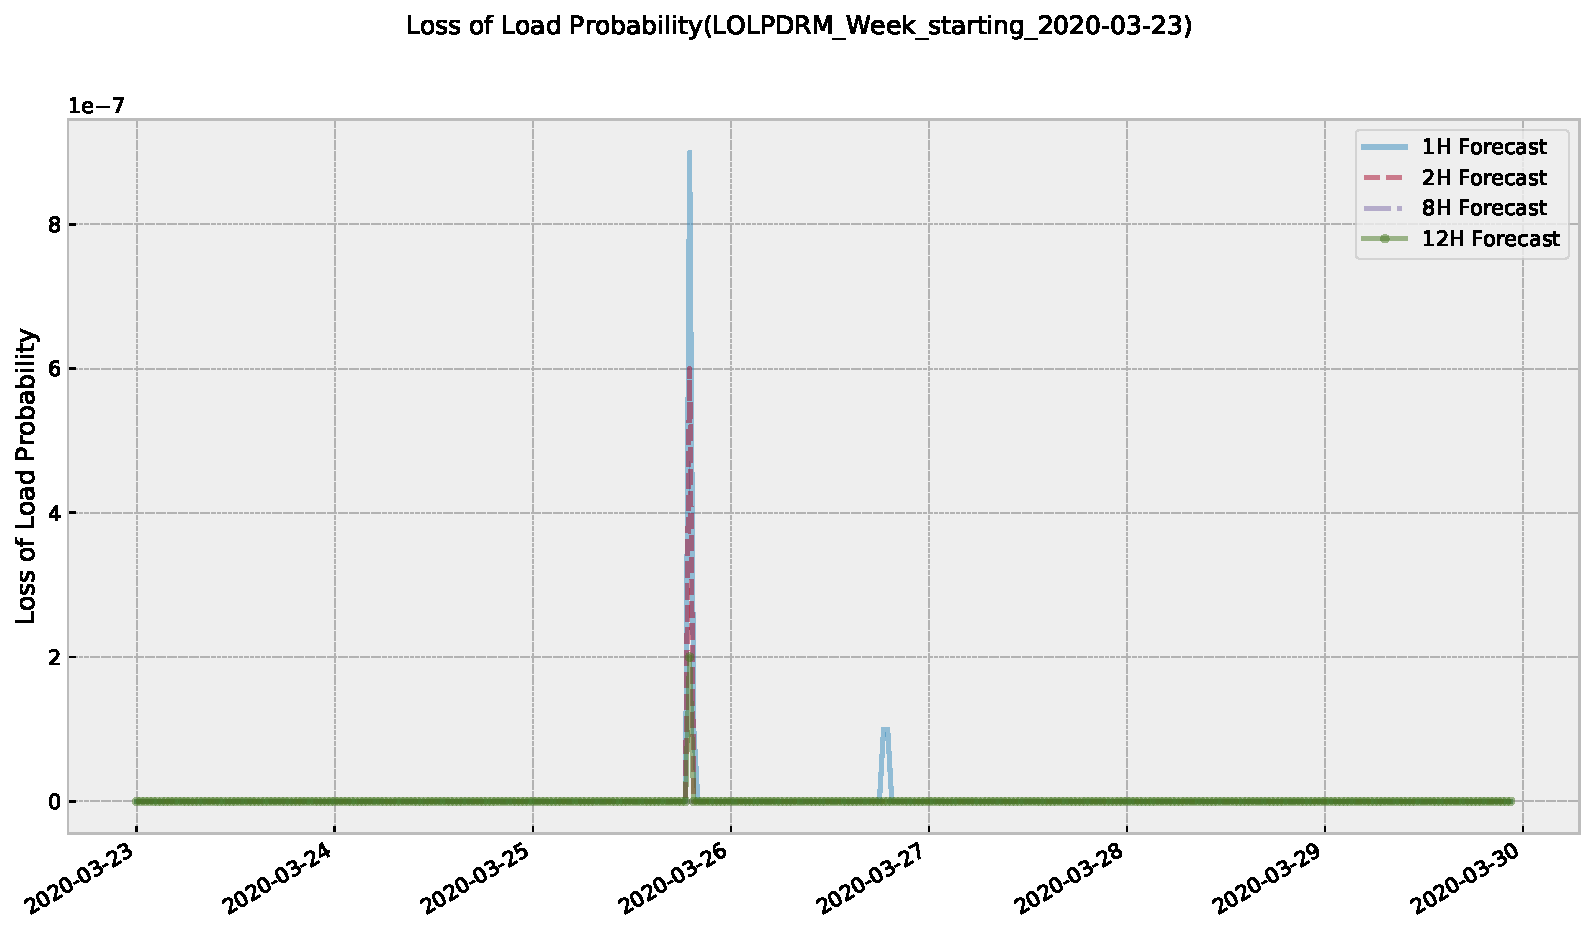
\includegraphics[width=15 cm]{Graphics/LOLPDRM_Week_starting_2020-03-23no4H.pdf}
\caption{LOLP variation Pre and Post.}\label{fig:LOLP_25_03}
\end{figure}  

% \subsubsection{Network constraints}\label{section: network constraints}
% The electrical network loading's will decrease on average but some network sections might reveal higher utilisation. The lower average demand in GB, imply less energy is transported through the power lines which results in reduced network loads. However, some other network sections could increase in loading as centralised renewable energy sources will transport energy for longer distances. The reason for longer transported energy is the lower electricity consumption closer to the VRE generators. For instance, the massive wind capacities installed in Great Britain's North - i.e. Scotland, providing energy up the southern part - i.e. London; when the net consumption in GB decreases, less energy will be directly consumed in the north and lead finally to higher network loads along the transmission lines at high wind and solar times. Therefore, even when the load in most networks will decrease some networks might experience the contrary.

%%%%%%%%%%%%%%%%%%%%%%%%%%%%%%%%%%%%%%%%%%%%%%%%%%%%%%%%%%%%%%%%%%%%%%%%%%%%%%%%
%\subsection{Ancillary Services/Demand-side Response}
%%%%%%%%%%%%%%%%%%%%%%%%%%%%%%%%%%%%%%%%%%%%%%%%%%%%%%%%%%%%%%%%%%%%%%%%%%%%%

\subsection{The effects on Market Price}\label{section:Market price}

%%%%%%%%%%%%%%%
\subsubsection{Day-ahead wholesale market price}\label{sec:day-ahead wholesale market price}

The day-ahead market objective is to define a clearing energy price in which supply meets the demand at any given hour of the day. To do so, a merit order model is used to correctly dispatch power plants by sorting the existing generation units from low to high marginal operating costs. Once the generation meets the demand curve the clearing market price or equilibrium is achieved by minimising the generation cost \cite{Maekawa2018TheExchange}. Figure \ref{fig:wholesale-market-effects} shows graphically the process of the merit order model and the location of the clearing price as a result of the intersection of the supply and demand curves. The demand is given as net demand which subtracts the VRE generation from the total demand. This is a common strategy to illustrate the merit-order, since the solar and wind generation plants have marginal cost close to zero, making them always dispatched so far no network or other operational constraints exist \cite{Hirth2014TheVariability}. 

\begin{figure}[H]
\centering
\hspace{-25pt}
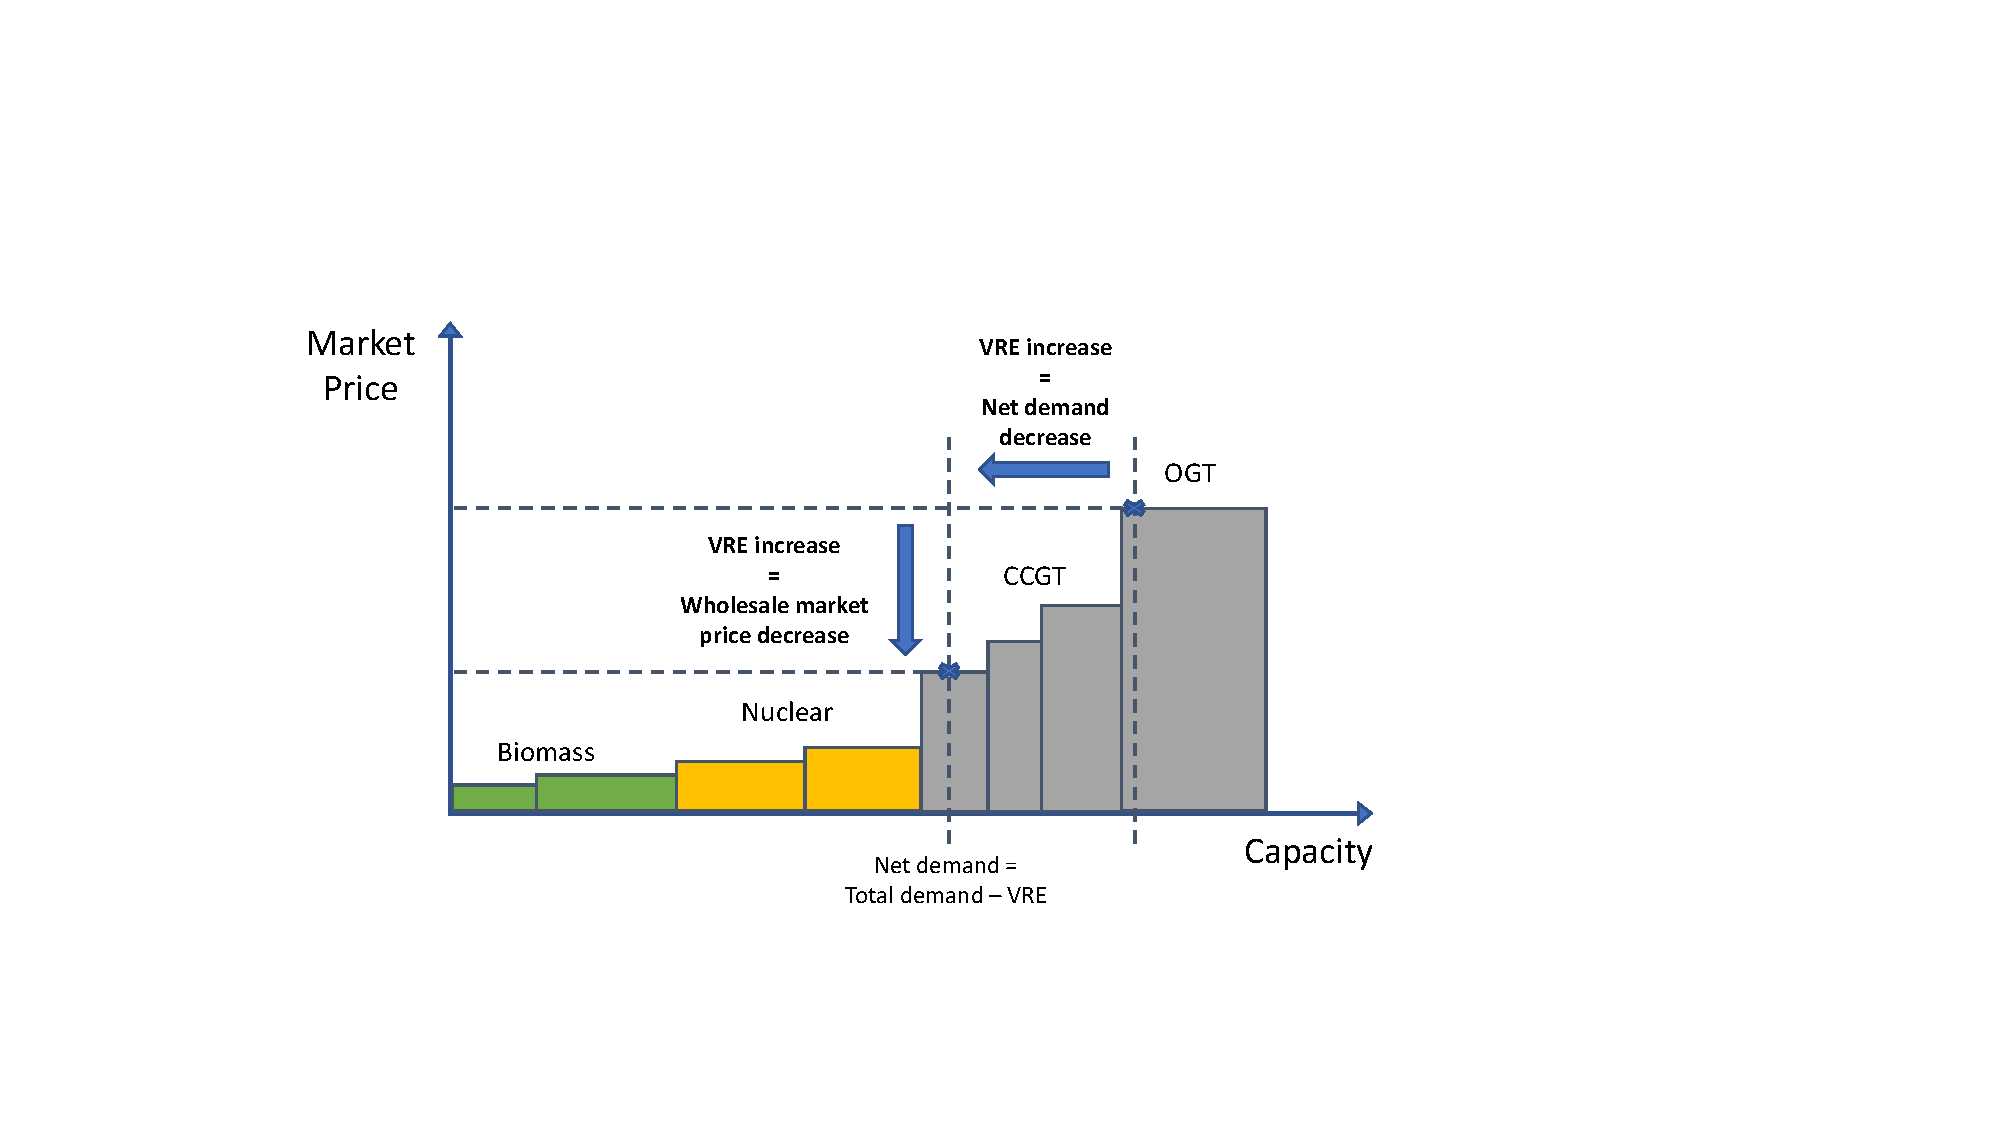
\includegraphics[trim={5cm 3cm 10cm 4.5cm},clip,width=13cm]{Graphics/Wholesale-market-price.pdf}
\caption{Illustrative effects of the COVID-situation on the wholesale market price.}
\label{fig:wholesale-market-effects}
\end{figure} 


\subsubsection{System imbalance price}\label{sec:system imbalance price}

The imbalance price is the price set by the system operator for every settlement period to determine imbalance charges on electricity producers (generators) or consumers (suppliers) \cite{ELEXON2019GuidanceBritain}. Whereby the imbalance charge for a settlement period simply consist of the product of imbalance volume (see section \ref{section:ImbalanceVolume}) and imbalance price:

\[ \text{Imbalance charge}_{SP} = \text{Imbalance volume}_{SP} \times \text{Imbalance price}_{SP} \]

To understand possibles impacts of the COVID situation on the imbalance price, it dismantled in its components. The imbalance price is the price which must be paid for actions that the system operator choose to resolve the imbalance. However, the reason for the balancing action can vary. It could be either a i) energy balancing or ii) system balancing motivated action in the 30min settlement period \cite{ELEXON2019GuidanceBritain}. 

According to \cite{ELEXON2019GuidanceBritain}, the energy balancing action in the "Balancing Mechanism"(BM) make sure that the energy amount of the physical notification is accomplished. This type of balancing action is usually priced by Bid-Offer scheme. The merit-order wise choice of Bid-Offers, meaning cheap actions first, is preferred to reduce the balancing cost. Though, this is not always possible due to technical limitations of generators, demands and networks. An example for a technical limitation of a BM-generator is a non-suitable ramp-up rate, or a limitation for the network, an already congested line which would not allow more generation. Therefore, not only the cheapest BM Bid-Offer prices are selected or resolved by the system operator. In the BM, units are usually priced by the utilisation cost, however, short term operating reserves (STOR) take a special role for the stability and priced by the greater price between i) utilisation price or ii) reserve scarcity price. Whereby, the reserve scarcity price is the product of the Loss of Load Probability (LoLP) and Value of Lost Load (VoLL). 

For the purpose of energy balancing, the system operator might additionally purchase non-BM services as "Balancing Service Adjustment Action" \cite{Nationalgrid2017ProcurementSO}. Drivers for such an adjustment action could be a more economical or specific necessary balancing characteristics from non-BM services, such as ancillary services or "other services" according to \cite{Nationalgrid2018BalancingStatement}. These non-BM actions are priced in capacity or energy or both ways and form balancing service adjustment data, consists of adjusted buy and sell prices, which adjust the imbalance price of the previously described BM \cite{Nationalgrid2017ProcurementSO,Nationalgrid2018BalancingStatement}.

The system-balancing actions, otherwise, are only a part of the non-BM actions \cite{Nationalgrid2018BalancingStatement}. They describe balancing actions which keep the energy balance at every instance. For example, a wind power plant might generate the exact energy amount as contracted by the physical notification for the 30 min settlement period, however, its power might fluctuate and mismatch the demand in the settlement period which make system-balancing actions, such as activation's of non-BM STOR units, necessary \cite{Nationalgrid2018BalancingStatement}. The pricing scheme for the system-balancing actions is equal to the energy-balancing scheme for non-BM actions, described in the previous paragraph.  

Figure \ref{fig:imbalance-price-development}, illustrates the weekly averaged imbalance price development in 2020. The imbalance price dropped significantly in the first week of the lock-down, while increased in the following week significantly, hence, showing an unclear trend. As described in the above paragraphs, the imbalance price is a complex construct. Therefore, the impact of the lock-down on the imbalance price can just be qualitatively evaluated.

\begin{figure}[H]
\centering
\hspace{-25pt}
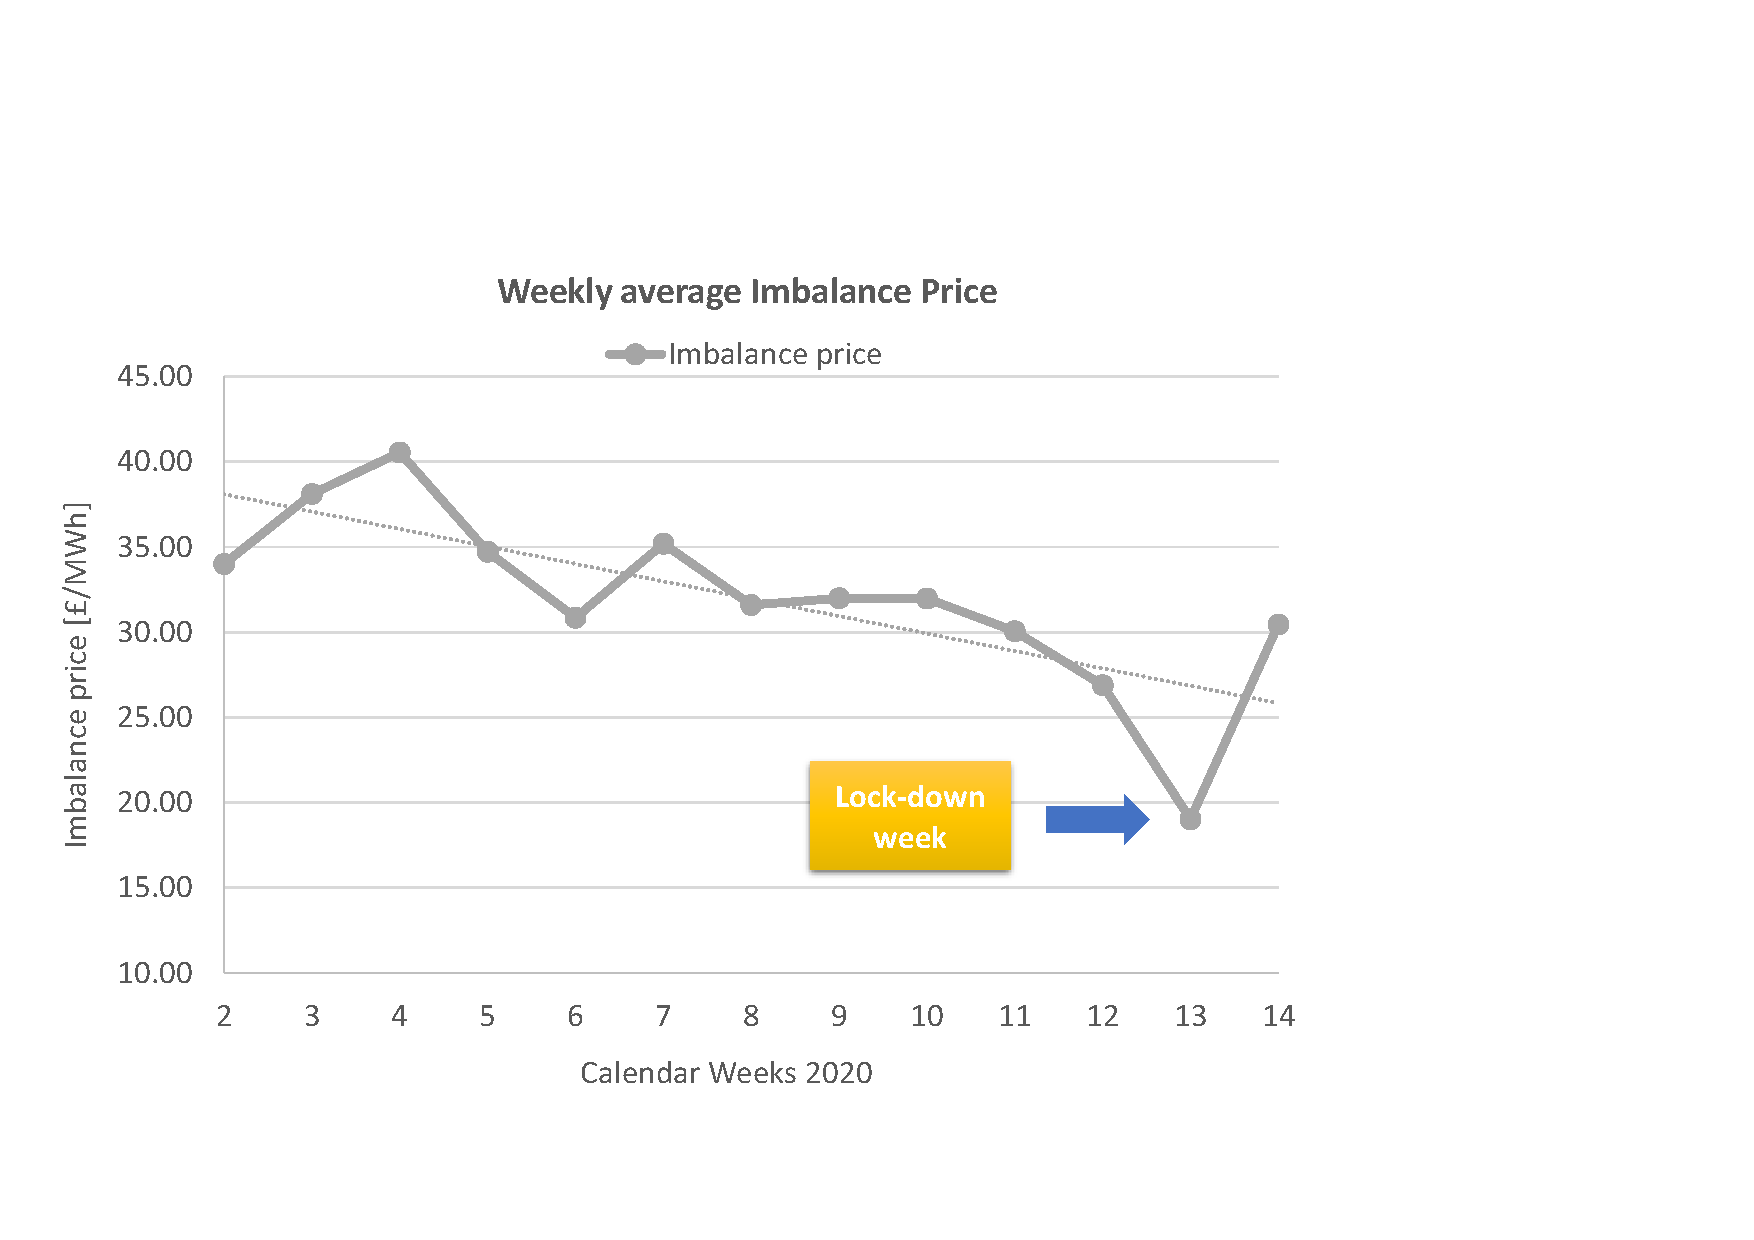
\includegraphics[trim={0cm 2cm 7cm 4.5cm},clip,width=0.8\textwidth]{Graphics/Imbalance-price-development-2020.pdf}
\caption{The impact of lower demand on the imbalance price}
\label{fig:imbalance-price-development}
\end{figure} 

The impacts of the lower demand at the lock-down times could potentially both increase and lower the imbalance price (see Fig. \ref{fig:imbalance-trade-off}). The balancing service options are generally chosen in a merit-order wise way, meaning activating cheap balancing options first, if no system operation limitation exists. Therefore, similar to a the wholesale market price settling, a higher demand would lead to higher prices and cheaper generators could lower the price or vice versa. That the imbalance volume could increase was explored in section \ref{section:ImbalanceVolume}, which imply a higher need for balancing services. Moreover, an on average lower demand as discovered in \ref{section: Effect on demand profile}, would potentially free up more generation units that can provide additional cost-effective balancing services. As result, the imbalance price could increase or decrease. The described effects frame not the whole picture, additionally investigation could be made on the LoLP, the VoLL, the de-rated margin, voltage related services and the network utilisation.

\begin{figure}[H]
\centering
\hspace{-25pt}
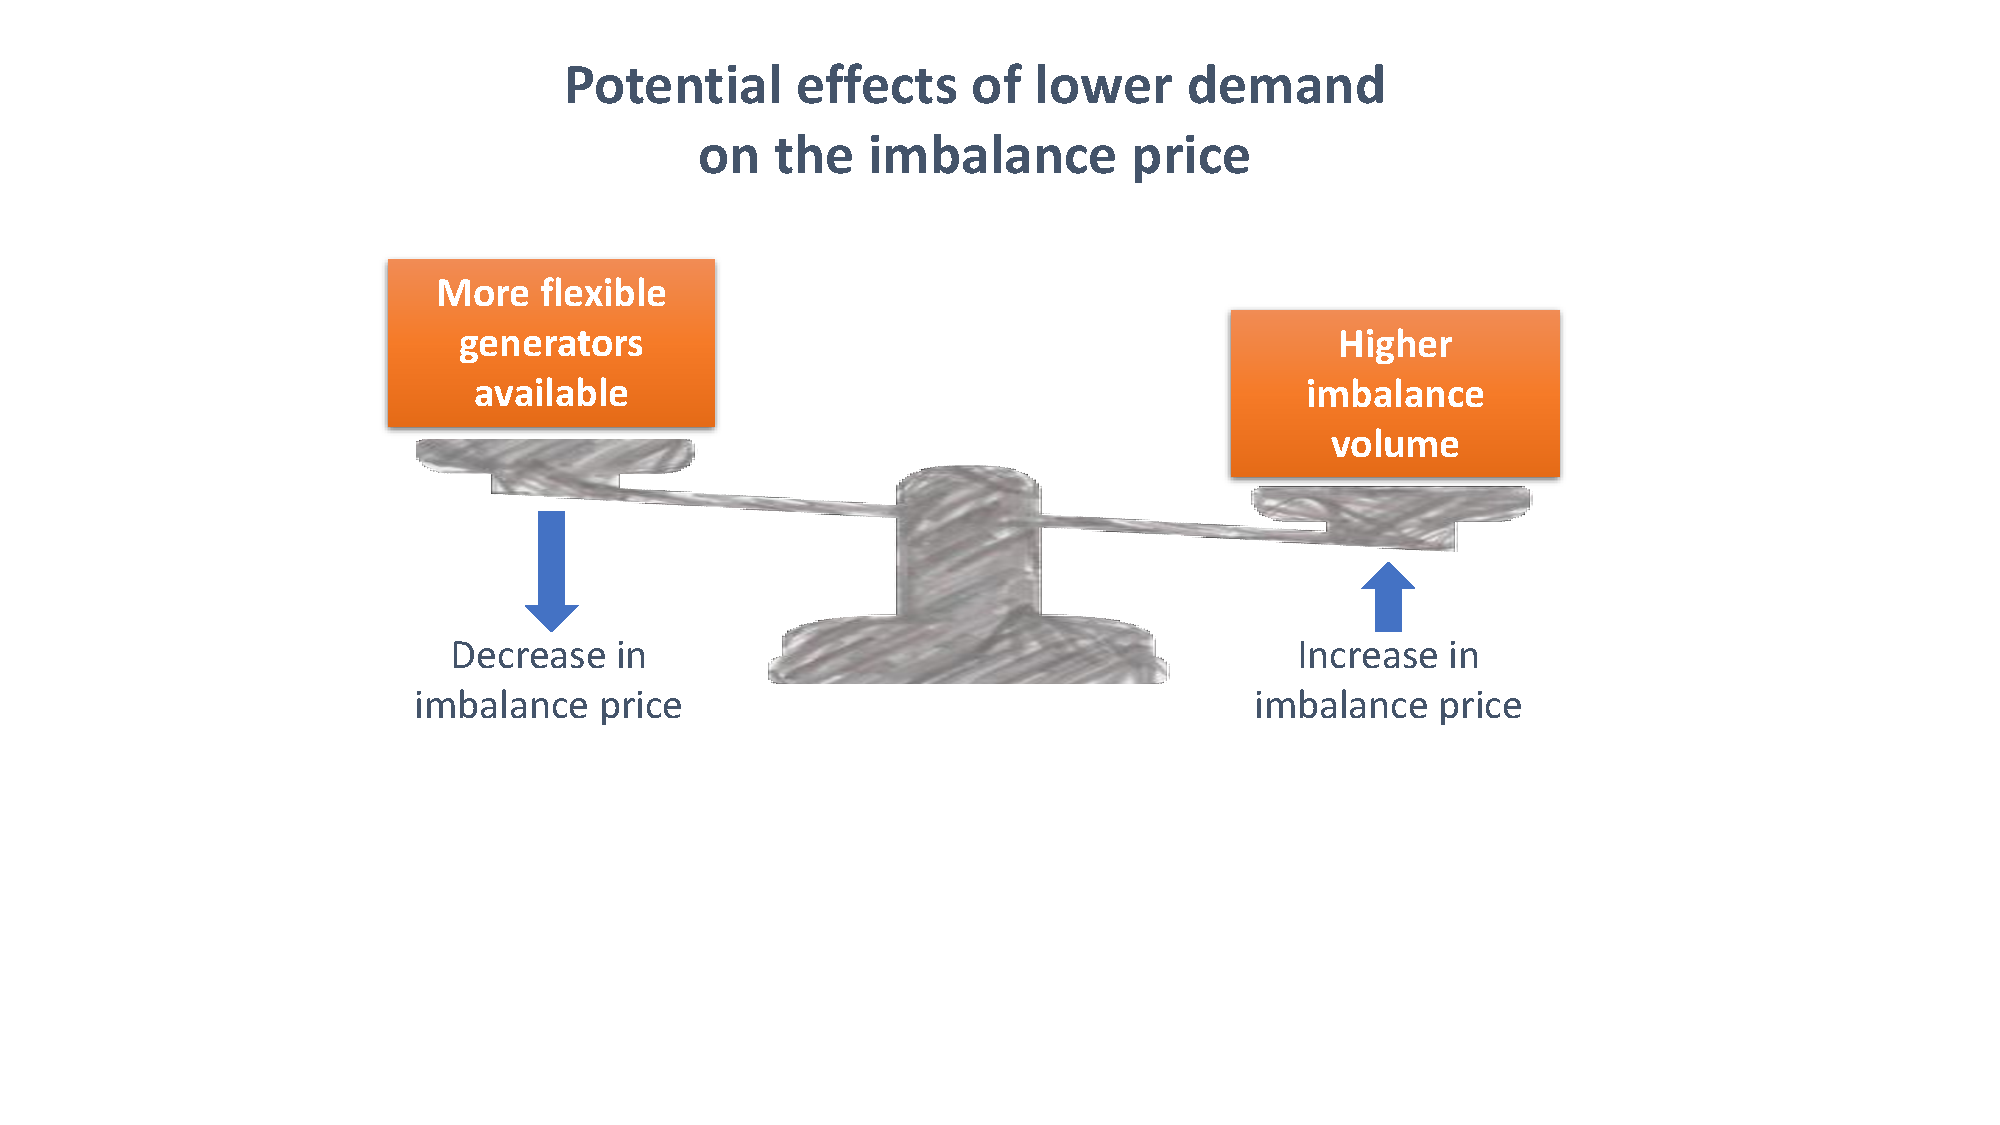
\includegraphics[trim={4cm 6.3cm 5cm 1cm},clip,width=13cm]{Graphics/Imbalance-price-trade-off.pdf}
\caption{The impact of lower demand on the imbalance price}
\label{fig:imbalance-trade-off}
\end{figure} 


%De-rate margin would be helpful.
%What is De-Rated Margin?De-rated Margin is a measure of the excess supply on the system, which has been adjusted to take account of the likely availability of plant, specific to each type of generation technology. %%%%"It reflects the proportion of an electricity source which is likely to be technically available to generate when needed"%%%%

%energy imbalance price calculation based on a theoretical set of balancing actions

%SO does not take all balancing actions for the same reason. 
%Some balancing actions are taken purely to balance the half hour energy imbalance of the Transmission System. These are ‘energy balancing’ actions.Other balancing actions are taken for non-energy, system management reasons. These are ‘system balancing’ actions.

%There are two energy imbalance prices for each Settlement Period. These are:System Buy Price (SBP); and System Sell Price (SSP).However there is a single price calculation, so SBP will equal SSP in each Settlement Period. ELEXON apply these prices to Parties’ imbalances to determine their imbalance charges. A Party is out of balance when its contracted energy volume does not match its physical production orconsumption.

\subsubsection{Variable Pricing for Domestic Consumers}
The case for variable pricing for domestic consumers was made by numerous studies \cite{REF!}. It is a more consumer-centric approach where the domestic consumers are billed using the same half-hourly prices as the commercial ones rather than having a fixed tariff (i.e. a volumetric calculation using a fixed £/kWh rate). There is also the commonly known time-of-use (ToU) pricing where the £/kWh rate varies for different times of the day which usually correlates to higher rates for higher demand periods. For instance, electricity prices from 4 to 7 p.m. would be higher to reflect the evening peak whereas from 1 am to 4 am when the demand is usually low, the prices would be lower. Hence, this method of pricing would also result in demand shifting.

A British energy supplier called Octopus \cite{AgileEnergy} introduced their "Agile" electricity tariff in which is an indexed half-hourly dynamic pricing that tracks the wholesale price of electricity (i.e. the domestic rate paid changes every 30 minutes instead of a fixed monthly rate). On different occasions, this has resulted in negative pricing (i.e. the energy supplier paid its customers to consume electricity). However, this also means that there is usually a steep price from 4pm to 7pm during the evening consumption surge. The following logic in Eq. \ref{eq:Octopus}, is used to determine the prime time pricing \cite{AgileEnergyb}. It uses the distribution cost coefficient ($\tau$) multiplied by the wholesale cost of electricity ($W$) and $P$ which is the peak-time premium (which is equal to 12p/kWh during prime time). Then it caps the price to £35p/kWh if the previous outcome is higher than this value \cite{AgileEnergyb}. This is because on average the fixed tariff are in the range of 15-20p/kWh and it could be argued exposing domestic consumers to extreme fluctuations in the system would be unfair.

\begin{equation}\label{eq:Octopus}
min((\tau \times W + P), 35p/kWh)
\end{equation}

% Octopus GO
In Figure \ref{fig:neg_agile}, an example of capping at the maximum price of 35p/kWh is shown on the 4\textsuperscript{th} of March 2020 (i.e. during the pre-COVID-19 week). This day marks the first time a system price was over £2,000/MWh since 2001. It peaked at £2,242/MWh \cite{ELEXONELEXONb} (See \ref{LOLPDRM_Week_starting_2020-03-23no4H} for the LOLP plot and visit Section \ref{section:LOLP_DRM} for more information). The week commencing on the 30\textsuperscript{th} of March 2020 is of interest for comparison with the other extreme, namely negative pricing, as it drops to near -3 pence per kilowatt-hour. Similar to the analysis in Section \ref{section: Effect on demand profile}, the reduction in demand magnitude and changes in profile are correlated to the changes between pre- and post-action pricing profiles in Figure \ref{fig:neg_agile}.

\begin{figure}[H]\centering
\hspace{-25pt}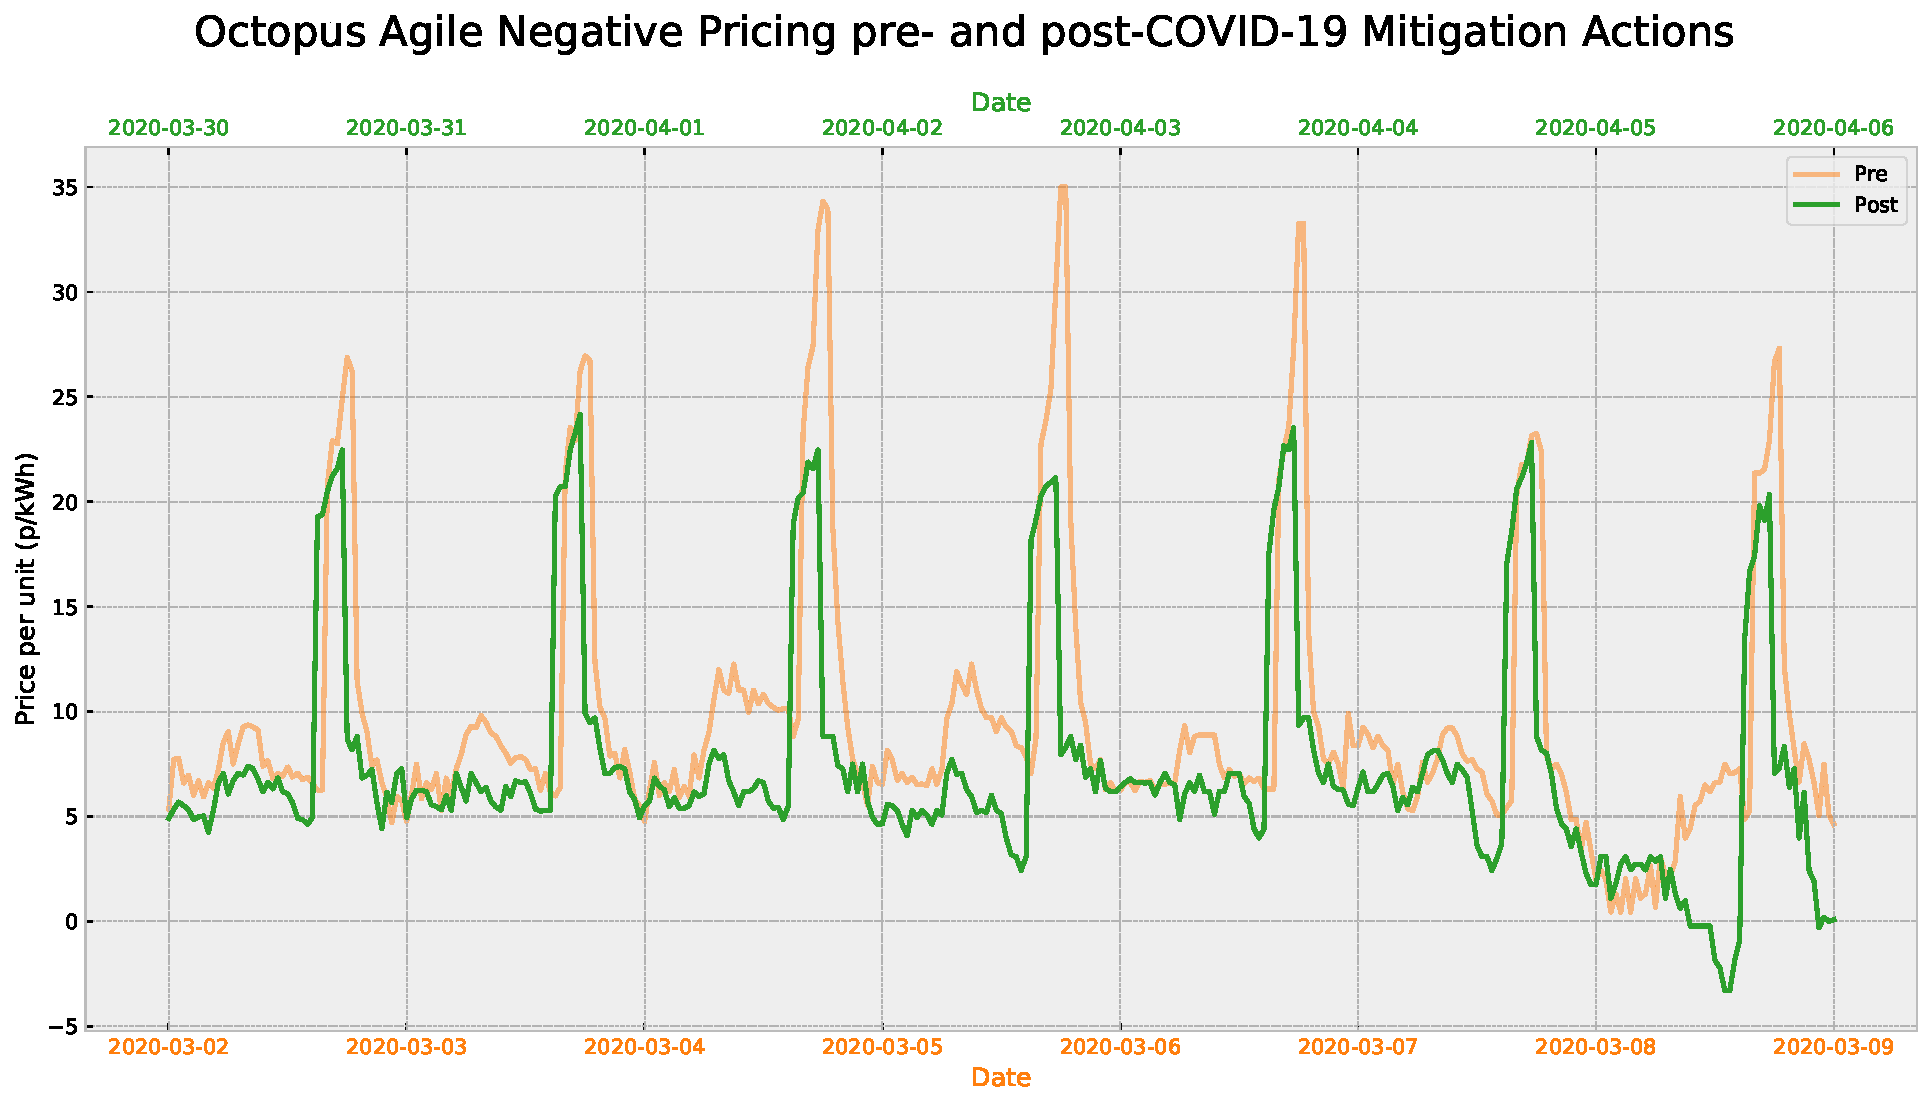
\includegraphics[trim={0 0 0 1.5cm}, clip,width=15 cm]{Graphics/Pre-post_Agilecomp_negative.pdf}
\caption{Examples of price capping and negative pricing during pre- and post-COVID-19 weeks respectively -using the data from \cite{HomeUK}.}\label{fig:neg_agile}
\end{figure}  

% The system price for the balancing mechanism peaked at £2,242/MWh  which marks the first time a system price is over £2,000/MWh since 2001 \cite{ELEXONELEXONb}. 



Since the launch of the Agile tariff, there has been 96 occurrences of negative pricing (i.e. price < 0p/kWh). Almost 70\% of these events (i.e. 67 out of 96) took place post-COVID-19 actions. Table \ref{table:neg_agile_table} summarises the pre and post negative pricing events highlighting the highest price the consumers were paid to use electricity and the corresponding dates.

\begin{table}[H]
\caption{Analysis of negative pricing in the  Agile tariff -using the data from \cite{HomeUK}}\label{table:neg_agile_table}
\centering
%% \tablesize{} %% You can specify the fontsize here, e.g., \tablesize{\footnotesize}. If commented out \small will be used.
\begin{tabular}{ccccc }
\toprule
\textbf{Data} & \textbf{Mean}	& \textbf{Min}	& \textbf{Max}& Dates corresponding to max values\\
\midrule
Pre	(p/kWh)	& -1.62			& -0.07         & -4.85 &09-12-2019\\
Post (p/kWh) & -1.36			& -0.02         & -3.99& 20-04-2020\\
Overall (p/kWh) & -1.44			& -0.02         & -4.85 &09-12-2019\\
\bottomrule
\end{tabular}
\end{table}

Octopus also provides variable pricing for selling electricity \cite{AgileEnergy}. The corresponding sell prices are plotted in Figure \ref{fig:agile_OUT}. The highest sell price around 19p/kWh was recorded which corresponds to the day with the highest system price since 2001. The benefit is passed on to the distributed generators. In the case of negative load pricing when the consumers were paid to use electricity on the 5\textsuperscript{th} of May, there would also negative pricing for exporting electricity (i.e. generators pay to export electricity). The pricing for generation is capped at a minimum of 0p/kWh which indicates that the energy was exported for free during that period as shown in Figure \ref{fig:agile_OUT}.

\begin{figure}[H]\centering
\hspace{-25pt}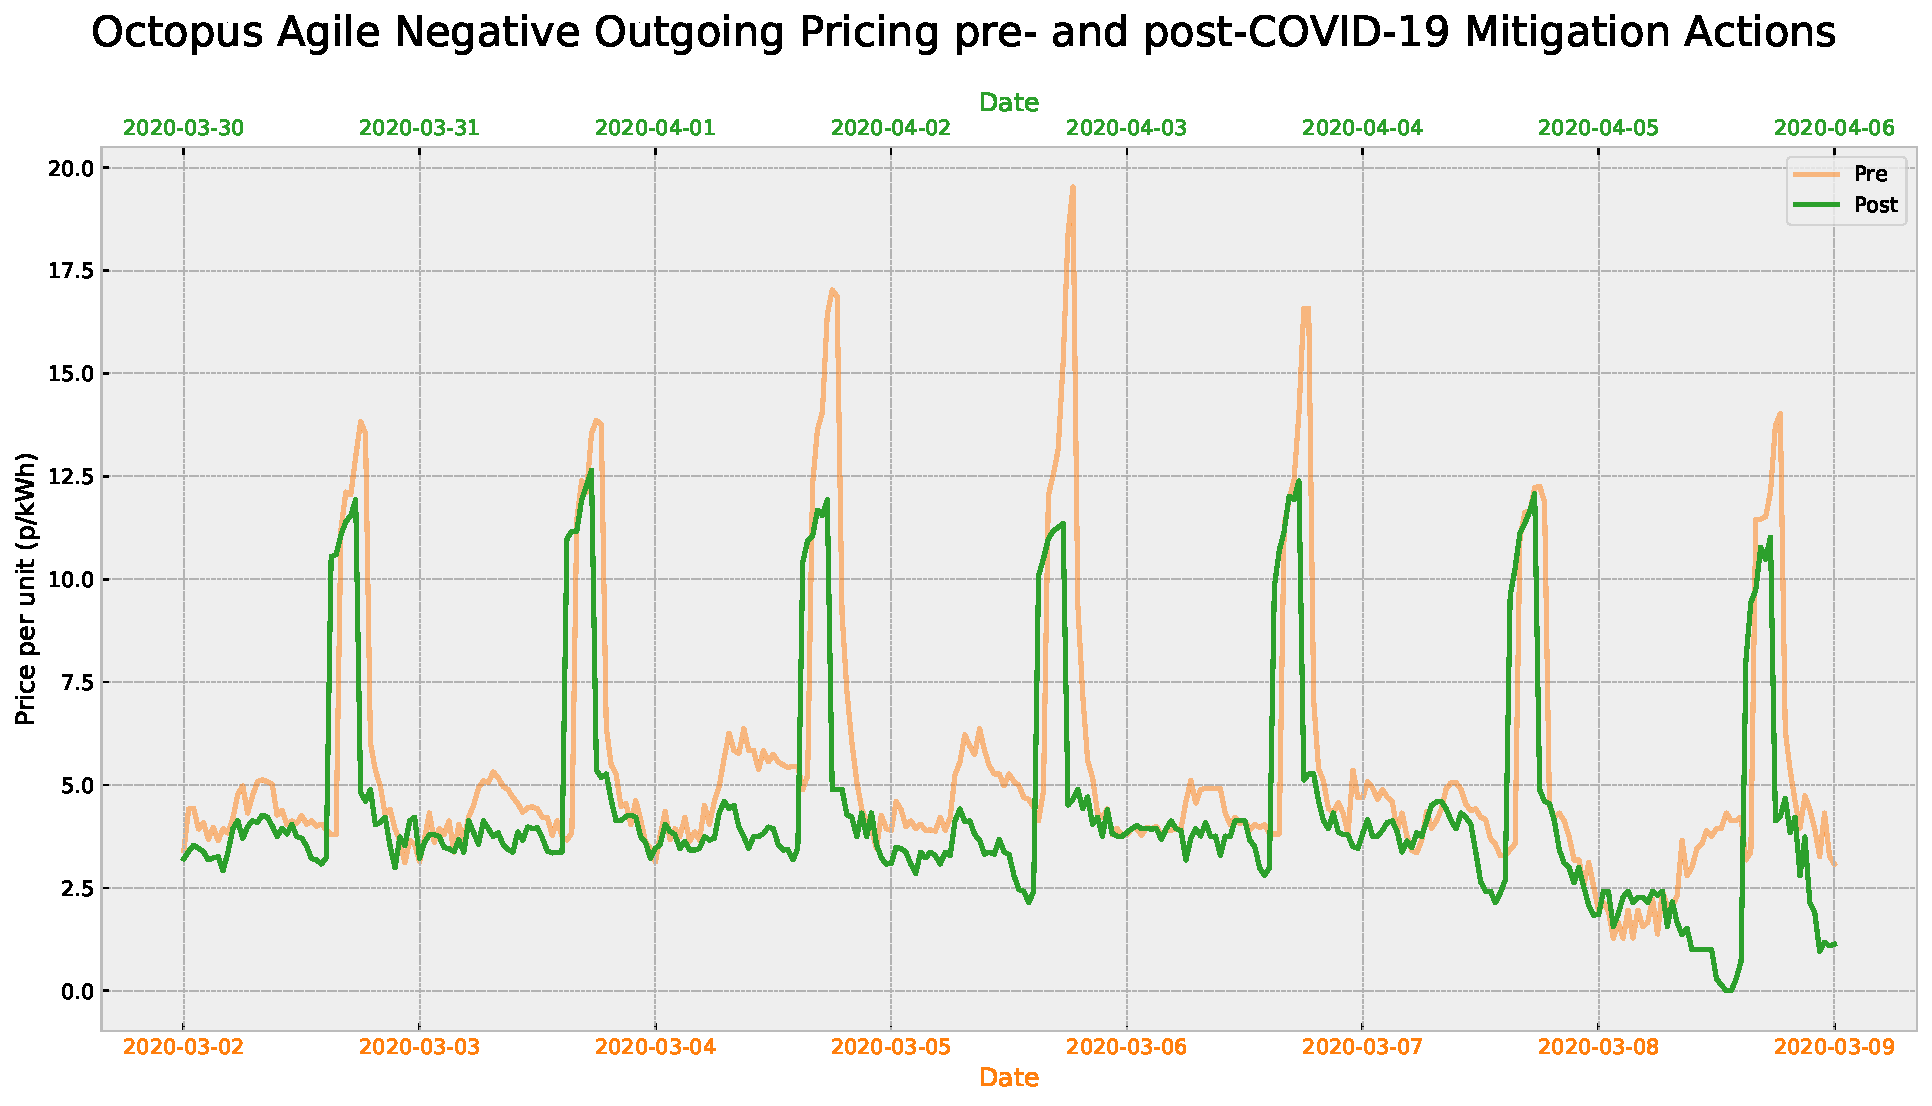
\includegraphics[trim={0 0 0 1.5cm}, clip, width=15 cm]{Graphics/Pre-post_AgileOUTGO_negative_comp.pdf}
\caption{Corresponding Agile outgoing sell prices.-using the data from \cite{HomeUK}}\label{fig:agile_OUT}
\end{figure}  

%===============================================================
%                           DISCUSSION
%===============================================================

\section{Discussion}
%%%%%%%%%%%%%%%%%%%%%%%%
%Dos
   % Summarise the key findings
   % Interpretations: what do the results mean?
   % Implications: why do the results matter?
   % Limitations: what can’t the results tell us?
   % Recommendations: what practical actions or scientific studies should follow?
%Don'ts
   %Don’t introduce new results
   %Don’t make inflated claims
   %Don’t undermine your research
 %%%%%%%%%%%%%%%%%%%%%%%%%%%%%%%%%%%%%%%%%  

The IEA estimates, we are looking now one decade into the future power system, when the share of VRE, such from solar and wind, is much higher and where balancing services are more demanded \cite{IgorTodorovic2020Birol:Balance}. The results in this paper summarised in Table \ref{table:Summary key results} indicate that the grid is still reliable and stable but stressed, and that the wholesale market price could drop. Indeed, we are experience due to COVID larger shares of VRE in the electricity system which requires more balancing services as the mismatch between supply and demand increased on average. But are we looking really into the future power system? 

Several indicators suggest that the current situation in GB cannot be compared with the future high renewable power system. First, the lock-down changed the load profile shape which make it smoother than in typically future scenarios. These smoother demand profile, counter-intuitively, lead to better day-ahead load forecast even though the share of VRE increased. Second, the current power system is backed by inflexible nuclear and coal plants which might change in future due to the growing amount of flexibility services such as DSR, aggregated generators and storages. Lastly, the network is at the moment comparatively oversized due to the lower load. The same network at higher VRE share could lead to more network congestion in a future power system.

Nevertheless, the inconvenient COVID situation could imply two future important points: The imbalance could increase, stressing the grid stability if the TSO is not prepared; and that network constraints might block smooth operation. Both points can be a more severe problem in the future power system which should be anticipated by system operators. 
 
\begin{figure}[H]
\centering
\hspace{-25pt}
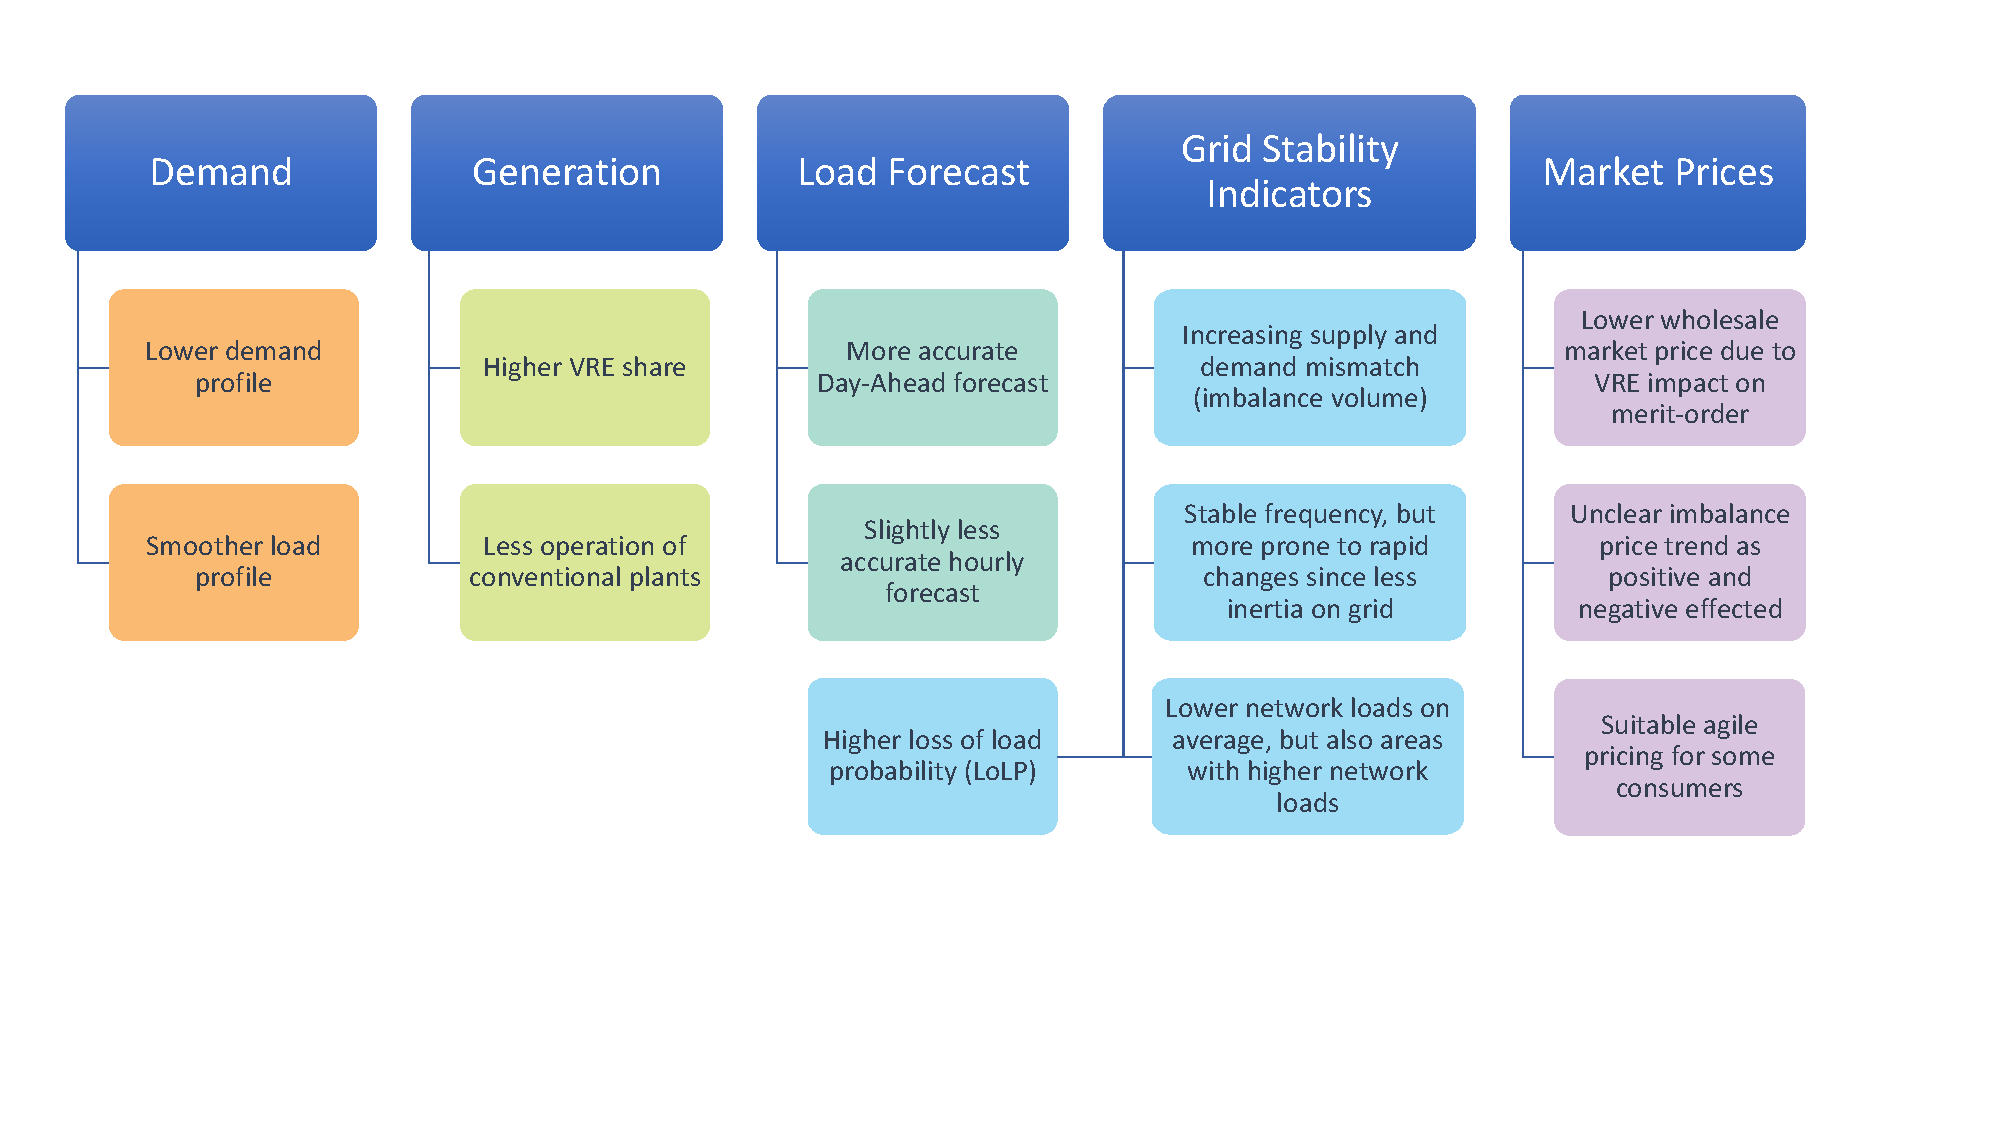
\includegraphics[trim={1cm 4.5cm 0cm 1.5cm},clip,width=1.1\textwidth]{Graphics/Key-findingsV3.pdf}
\caption{Summarised key results}
\label{fig:key-results}
\end{figure} 

\begin{table}[H]
\caption{Summarised key results.
}\label{table:Summary key results}
\centering
%% \tablesize{} %% You can specify the fontsize here, e.g., \tablesize{\footnotesize}. If commented out \small will be used.
\begin{tabular}{cc}
\toprule
\textbf{Type} & \textbf{Result}	\\
\midrule

\multirow{2}{10em}{Demand}
& - Lower demand profile \\ 
& - Smoother load profile\\\\

\multirow{3}{10em}{Generation} 
& - Higher VRE share \\ 
& - Less operation of conventional plants \\ 
& - Inflexbile plants more likely pushed out of market \\\\

\multirow{2}{10em}{Load Forecast} 
& - Day-Ahead forecast more accurate due to smoother load profile \\
& - Hourly forecast slightly drops in accuracy  \\\\

\multirow{6}{10em}{Grid stability indicators} 
& - Frequency stable, but more prone to rapid changes since less inertia on grid \\
& - Higher loss of load probability (LoLP)\\
& - Demand and supply mismatch (imbalance volume) \\
& increases due to higher VRE share as significant 
driver \\ 
& - Network load lower on average but some areas \\
& with higher VRE share could reveal higher loads\\\\ 


\multirow{2}{10em}{Market prices} 
& - Wholesale market price, lower due to VRE impact on merit-order \\ 
& - Impact on system imbalance prices, unclear as \\
&price components are positive and negative effected \\ 
& - Agile prices, ???\\\\ 



\bottomrule
\end{tabular}
\end{table}



%%%%%%%Comments below%%%%%%%%%%%%

%\textcolor{blue}{
%NOTES from initial observations: Every day is a "weekend" -> Lower and delayed morning peak, lower evening peak - generally lower consumption.
%\begin{itemize}
%    \item System operator - Harder to predict the demand profile and peak - challenges the forecasting/predictive algorithms employed by National Grid
%    \subitem Did the machine learning algorithms/predictive control/etc. see this coming?
%    \item Aggregators and agents in DSR - may be making profit- due to these unforeseen changes in demand profile
 %   \item Generators - changes in scheduling - also not selling as much as they were promised as the demand decreased
%    \item Industrial and Domestic consumers - paying less? - fixed term contracts?
%    \item the impact of a shift from commercial and industrial load to largely domestic load
%\end{itemize}}

%\textcolor{blue}{
%\begin{itemize}
%    \item Due to the lower load caused by the lock-down, the average share of VRE increases in the power system. (important for discussion, as generally with higher VRE shares, i) prediction errors increase, ii) more ancillary services, iii) and the DA-clearance price decrease [already recognized from data])
%\end{itemize}
%}

\textcolor{blue}{
\begin{itemize}
    \item The head of the IEA, Fatih Birol, estimated that we are looking now one decade into the future power system, when the share of renewables is much more higher \cite{IgorTodorovic2020Birol:Balance}. This is not fully correct.
\end{itemize}
}

\subsection{Implications for Stakeholders}

The new disruptive and lower demand profile lead to multiple effects on stakeholders in the electricity system for network operators, supplier and generators, aggregators and DSR-provider, and consumers. 

The network operators will see on average lower network loads, occasionally higher network loads, and increasing activation of balancing services. First, higher amount of balancing services can be explained due to the observed performance drop in short-term forecasting (see Section \ref{DemandForecastError}) and the resulting higher volume of imbalances (see Section \ref{section:ImbalanceVolume}). To guarantee a reliable and stable grid, balancing services will be more often activated. Second, lower network loads are expected due to the lower average load at lock down times. Although, at some, particular high VRE locations, the network load might increase because of new power flows (see Section \ref{section: network constraints}).

In the wholesale market, customers (Suppliers) enter contracts with producers (Generators) which form together a Balancing and Settlement Code party \cite{ELEXON2019GuidanceBritain}. Since the imbalance due to rising load uncertainty and the load profile increases, these parties are more often faced to imbalance charges towards the system operator. The trend of the total amount of imbalance charges cannot be easily detected, as described in Section \ref{sec:system imbalance price}. The imbalance price is a complex measure which can increase and decrease due to the lock-down effects. 

Beside the imbalance, generators and suppliers, will suffer from the disruptive demand change in terms of profitability. The share of fix-cost compared to amount of sales will increase, leading eventually to higher electricity prices for domestic and industrial consumers. Contrary, supplier benefit from lower wholesale market prices, however, if this cost are transferred to the consumer is not guaranteed (see Section \ref{sec:day-ahead wholesale market price}).

Aggregators and Demand side response (DSR) providers are expected to be more often scheduled because of the larger imbalance volume observed after the lock-down. The only requirement for them is to be more competitive then the new entering flexibility's from the non-scheduled power plants. If so, aggregators and DSR providers will benefit from the COVID-19 crisis.

% \begin{figure}[H]
% \centering
% \hspace{-25pt}
% 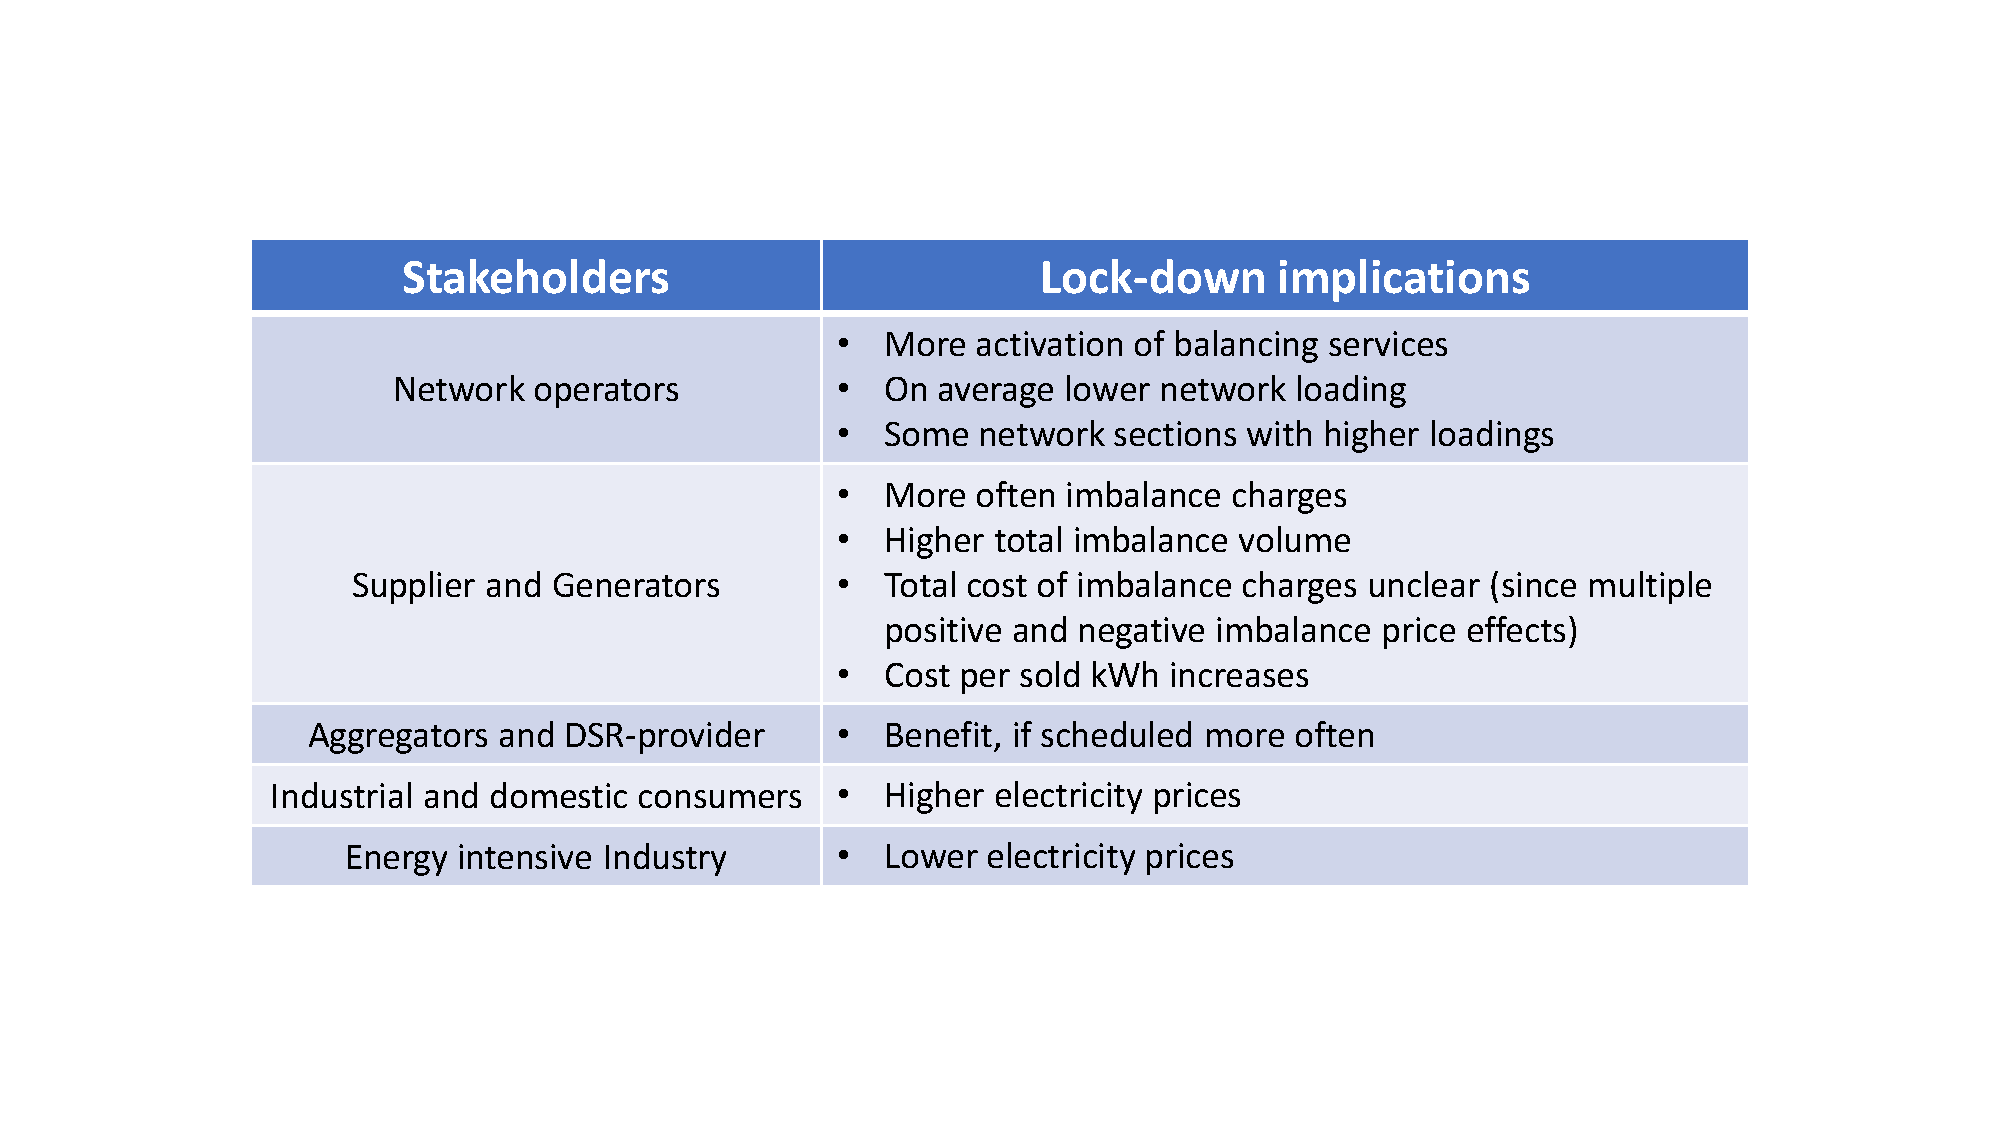
\includegraphics[trim={2cm 3cm 2cm 3.5cm},clip,width=1\textwidth]{Graphics/Stakeholder - lock-down implications.pdf}
% \caption{The implication of the lock-down on the various stakeholders}
% \label{fig:imbalance-price-trade-off}
% \end{figure} 



\begin{table}[H]
\caption{The implication of the post-COVID-19 electricity market for the stakeholders.
}\label{table:Implications}
\centering
%% \tablesize{} %% You can specify the fontsize here, e.g., \tablesize{\footnotesize}. If commented out \small will be used.
\begin{tabular}{cc}
\toprule
\textbf{Stakeholders} & \textbf{Implications}	\\
\midrule

\multirow{3}{10em}{Network Operators} 
& More activation of balancing services \\ 
& On average lower network loading \\ 
& Some network sections with higher loadings \\\\ 

\multirow{5}{10em}{Supplier and Generators} 
& Lower wholesale market price \\
& More often imbalance charges \\ 
& Higher total imbalance volume \\ 
& Total cost of imbalance charges unclear \\
& \textit{(single multiple positive and negative imbalance price effects)} \\ 
& Fix cost per generated or supplied kWh increases \\\\

\multirow{3}{10em}{Aggregator and DSR provider} 
& Benefit, if scheduled more often \\ \\ \\

\multirow{1}{10em}{Domestic and Industrial consumer} 
& Fixed pricing. Electricity price impact vague,\\ & since lower wholesale market prices might not be transferred by supplier \\\\ 


\multirow{2}{10em}{Domestic and Industrial consumer} 
& Variable pricing. ... \\\\ 



\bottomrule
\end{tabular}
\end{table}


%===============================================================
%                           CONCLUSIONS
%===============================================================
\section{Conclusions}

This section is not mandatory, but can be added to the manuscript if the discussion is unusually long or complex.
*copy from intro
*summarise contributions
***This paper encourages further research***

\vspace{6pt} 

%===============================================================
%                           MISC
%===============================================================

%%%%%%%%%%%%%%%%%%%%%%%%%%%%%%%%%%%%%%%%%%
%% optional
%\supplementary{The following are available online at \linksupplementary{s1}, Figure S1: title, Table S1: title, Video S1: title.}

%%%%%%%%%%%%%%%%%%%%%%%%%%%%%%%%%%%%%%%%%%
\authorcontributions{For research articles with several authors, a short paragraph specifying their individual contributions must be provided. The following statements should be used ``conceptualization, X.X. and Y.Y.; methodology, X.X.; software, X.X.; validation, X.X., Y.Y. and Z.Z.; formal analysis, X.X.; investigation, X.X.; resources, X.X.; data curation, X.X.; writing--original draft preparation, X.X.; writing--review and editing, X.X.; visualization, X.X.; supervision, X.X.; project administration, X.X.; funding acquisition, Y.Y.'', please turn to the  \href{http://img.mdpi.org/data/contributor-role-instruction.pdf}{CRediT taxonomy} for the term explanation. Authorship must be limited to those who have contributed substantially to the work reported.}

%%%%%%%%%%%%%%%%%%%%%%%%%%%%%%%%%%%%%%%%%%
\funding{Please add: ``This research received no external funding'' or ``This research was funded by NAME OF FUNDER grant number XXX.'' and  and ``The APC was funded by XXX''. Check carefully that the details given are accurate and use the standard spelling of funding agency names at \url{https://search.crossref.org/funding}, any errors may affect your future funding.}

%%%%%%%%%%%%%%%%%%%%%%%%%%%%%%%%%%%%%%%%%%
\acknowledgments{In this section you can acknowledge any support given which is not covered by the author contribution or funding sections. This may include administrative and technical support, or donations in kind (e.g., materials used for experiments).}

%%%%%%%%%%%%%%%%%%%%%%%%%%%%%%%%%%%%%%%%%%
\conflictsofinterest{The authors declare no conflict of interest. The funders had no role in the design of the study; in the collection, analyses, or interpretation of data; in the writing of the manuscript, or in the decision to publish the results.} 

%%%%%%%%%%%%%%%%%%%%%%%%%%%%%%%%%%%%%%%%%%
% %% optional
% \abbreviations{The following abbreviations are used in this manuscript:\\

% \noindent 
% \begin{tabular}{@{}ll}
% MDPI & Multidisciplinary Digital Publishing Institute\\
% DOAJ & Directory of open access journals\\
% TLA & Three letter acronym\\
% LD & linear dichroism
% \end{tabular}}

%%%%%%%%%%%%%%%%%%%%%%%%%%%%%%%%%%%%%%%%%%
%% optional
\appendixtitles{no} %Leave argument "no" if all appendix headings stay EMPTY (then no dot is printed after "Appendix A"). If the appendix sections contain a heading then change the argument to "yes".
\appendix
\section{Extras}

\begin{figure}[H]
\centering
\hspace{-25pt}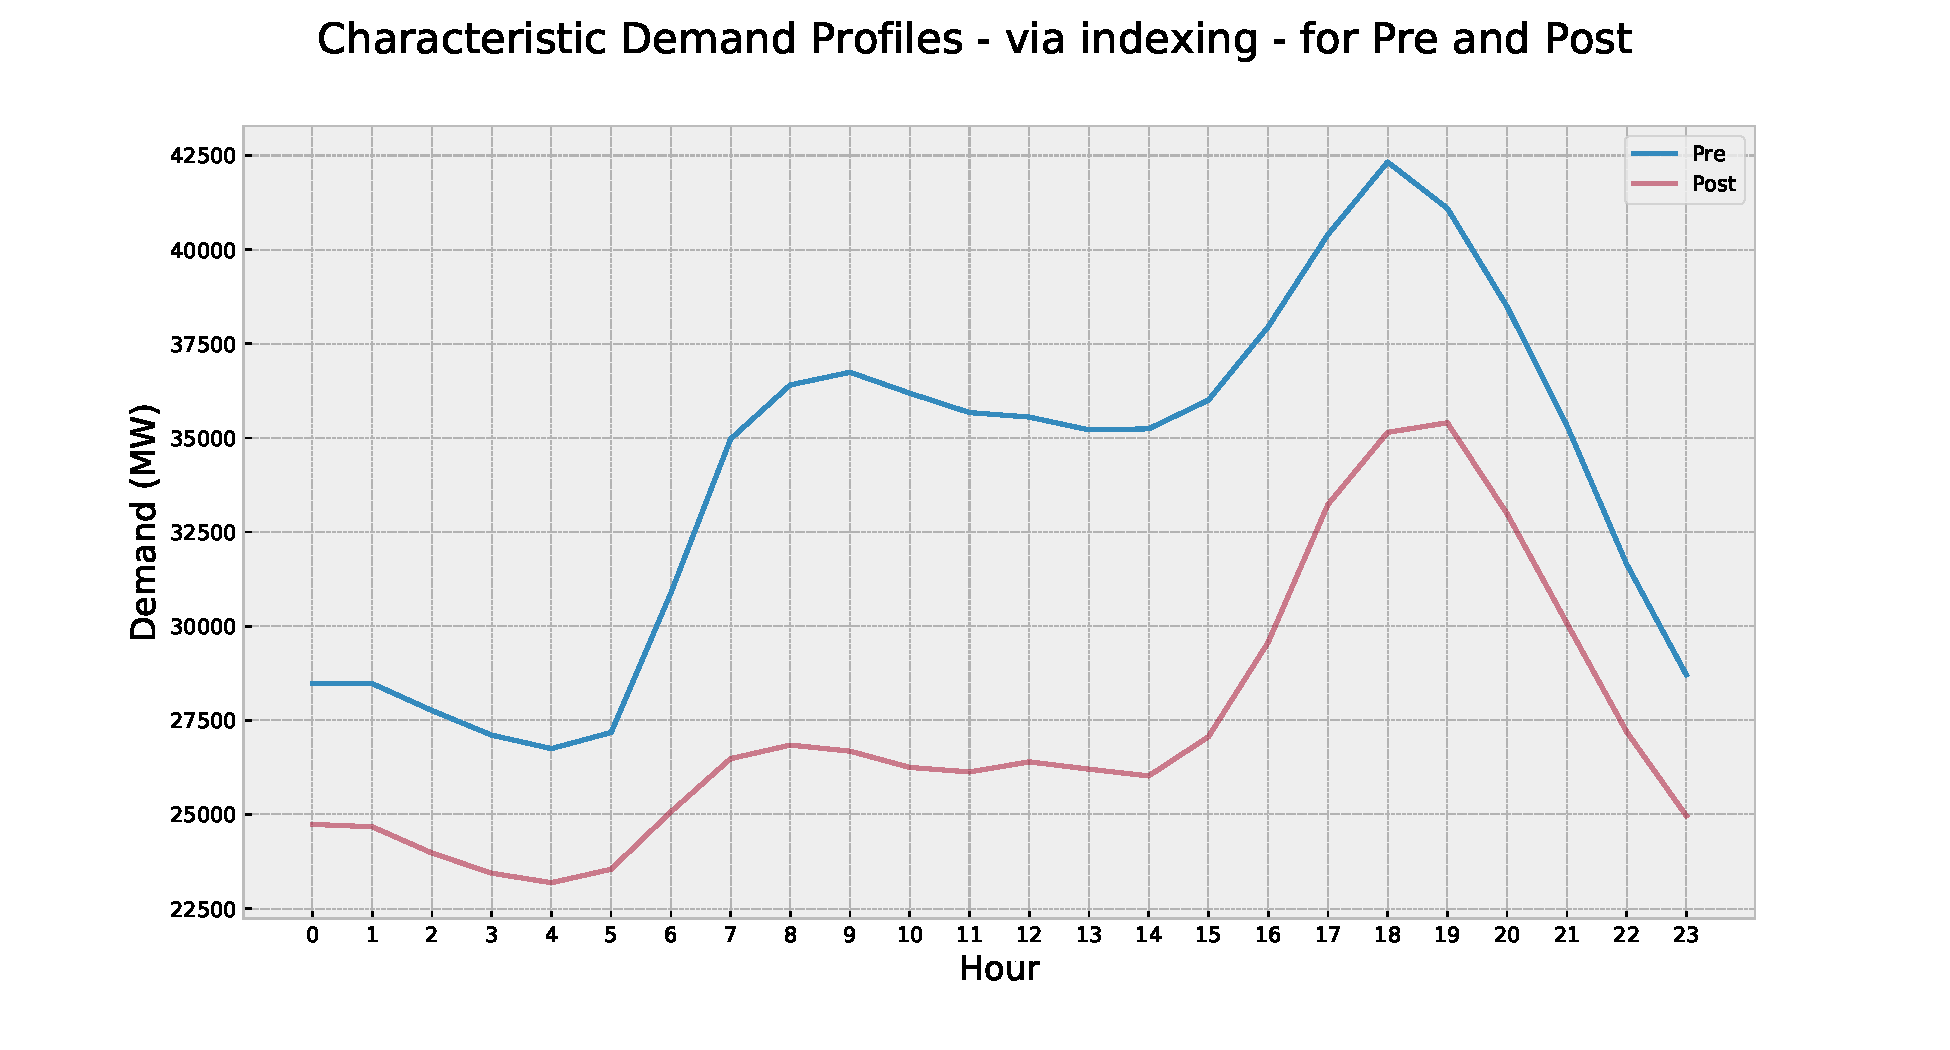
\includegraphics[width=15 cm]{Graphics/Characteristic_Profiles_pre_post.pdf}
\end{figure}

\section{The Data Pipeline\label{section:PipelineCode}}
%%%INSERT py file - auto-conversion will hopefully work here%%%%
% \lstinputlisting[language=Python]{source.py}

\section{Agile Tariff Plots}
For completeness, the plots for the pre and post-COVID-19 weeks (i.e. week commencing on the 2\textsuperscript{nd} and 23\textsuperscript{rd} of March 2020) used for demand and system frequency analysis are included.
\begin{figure}[H]
\centering
\hspace{-25pt}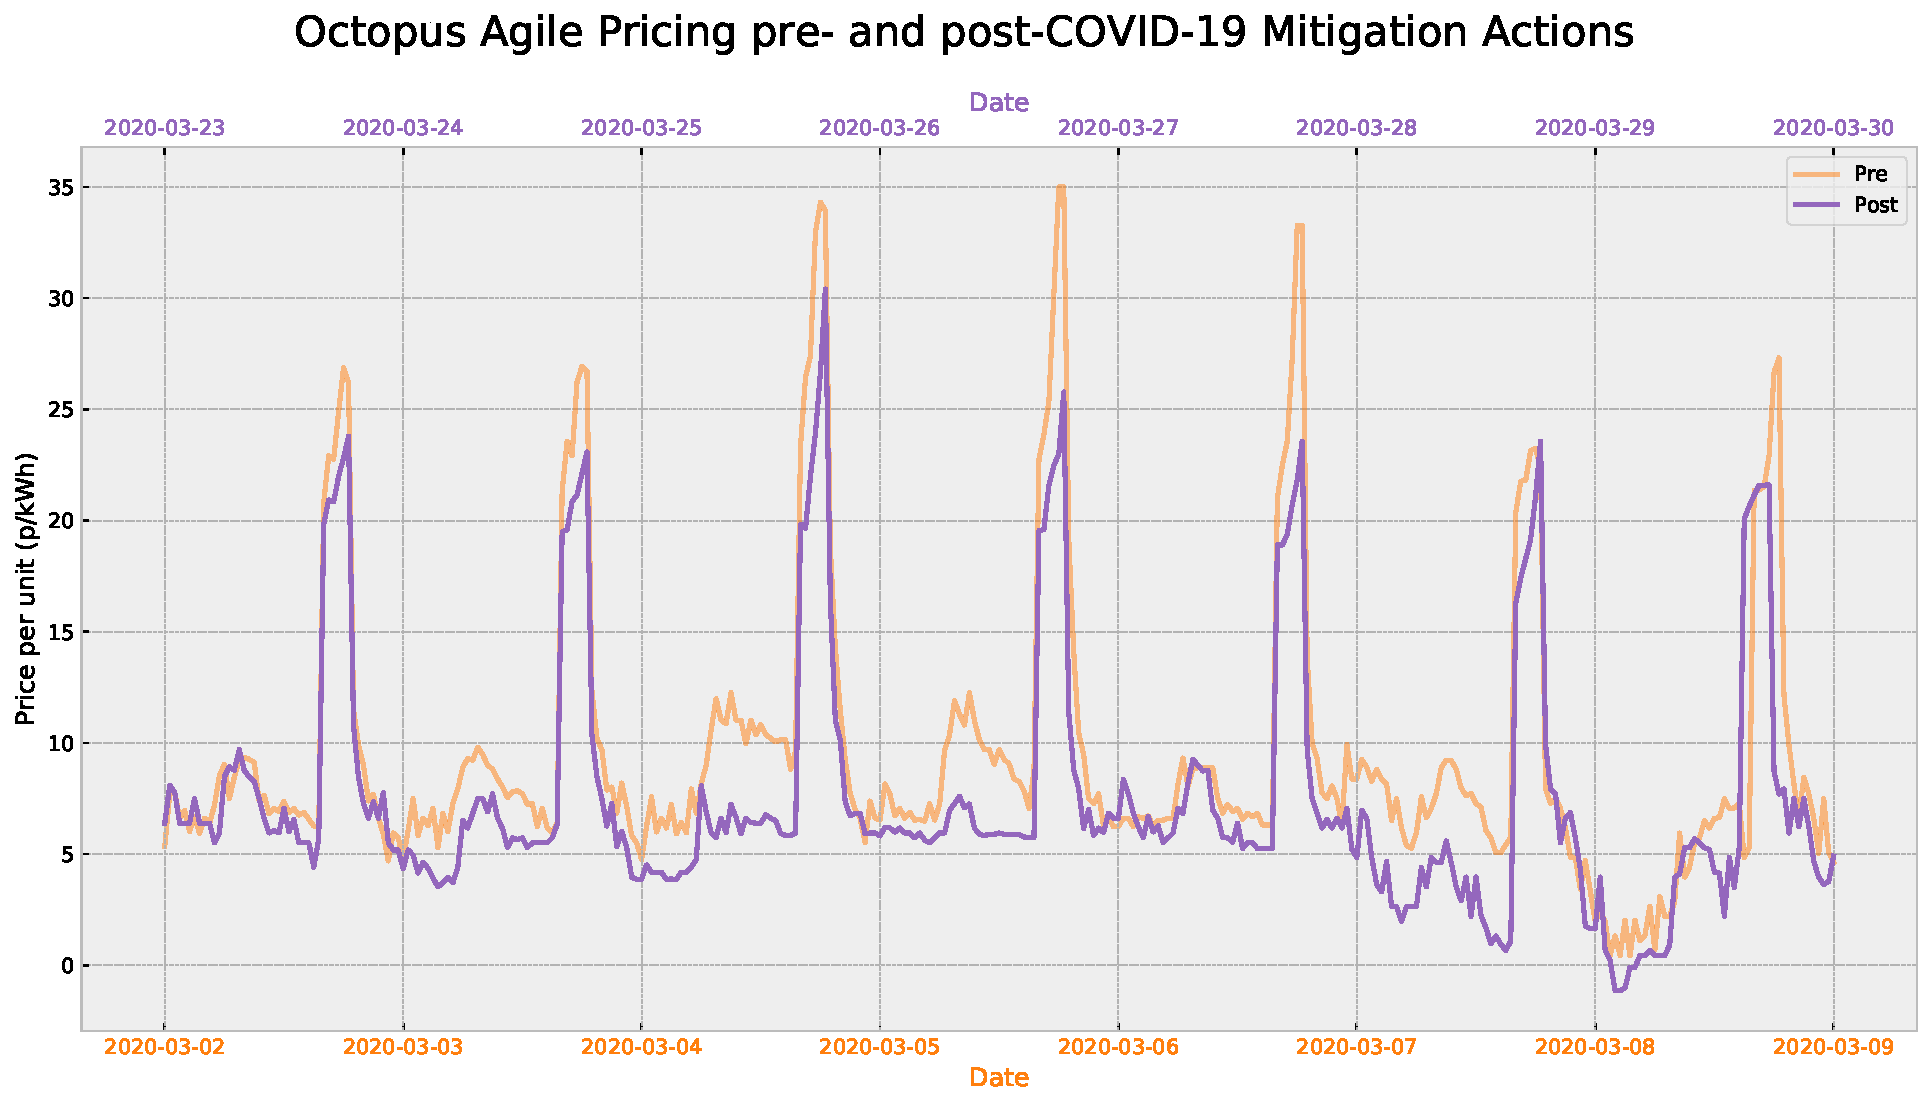
\includegraphics[width=15 cm]{Graphics/Pre-post_Agilecomp.pdf}
\caption{Octopus Agile Pricing comparison of before and after the COVID-19 actions.-using the data from \cite{HomeUK}}\label{fig:agile_comp_prepost}
\end{figure}

\begin{figure}[H]\centering
\hspace{-25pt}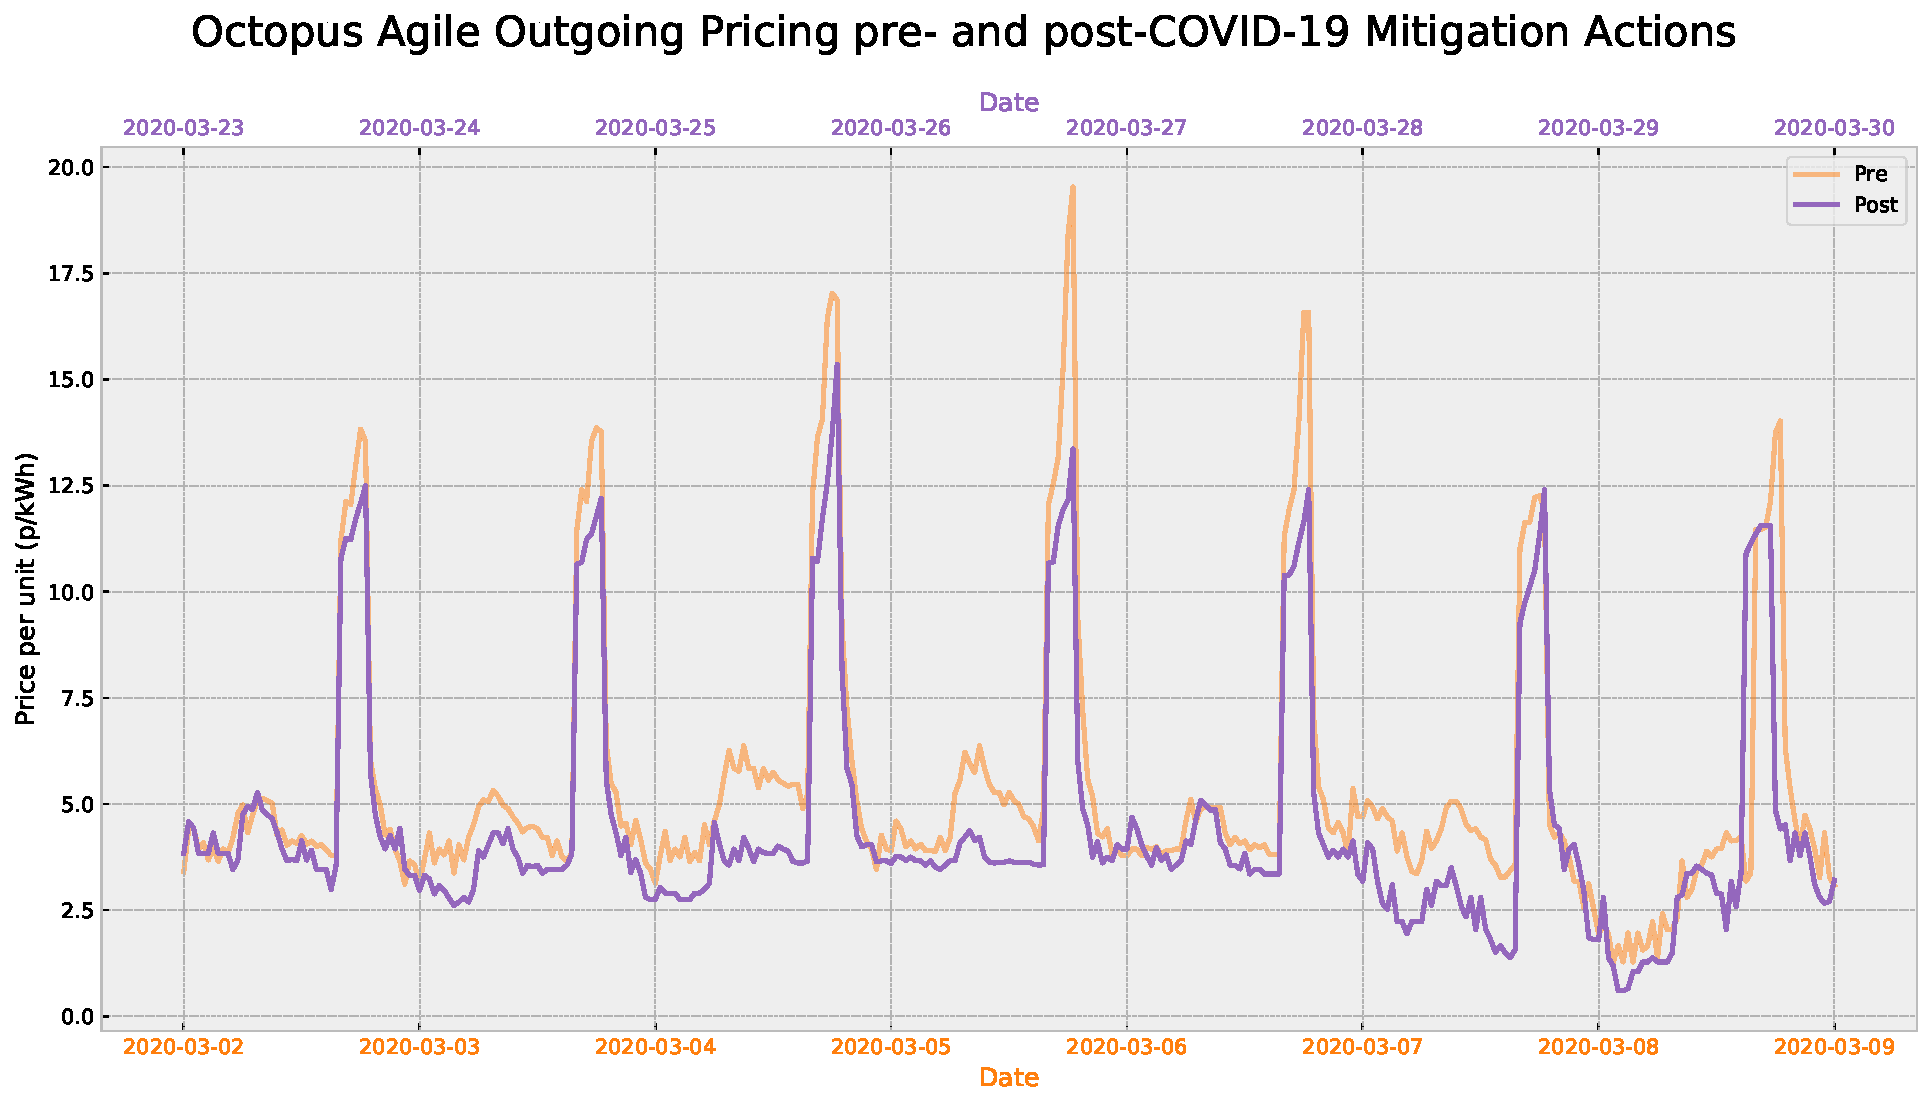
\includegraphics[width=15 cm]{Graphics/Pre-post_AgileOUTGO_comp.pdf}
\caption{Octopus Agile sell pricing comparison of before and after the COVID-19 actions.-using the data from \cite{HomeUK}}\label{fig:agile_OUT_comp_prepost}
\end{figure}  
\section{LOLP Plots}
For completeness, the LOLP plots for the pre and post-COVID-19 weeks (i.e. week commencing on the 2\textsuperscript{nd} and 23\textsuperscript{rd} of March 2020) used for demand and system frequency analysis are included.
% \begin{figure}[H]\centering
% \hspace{-25pt}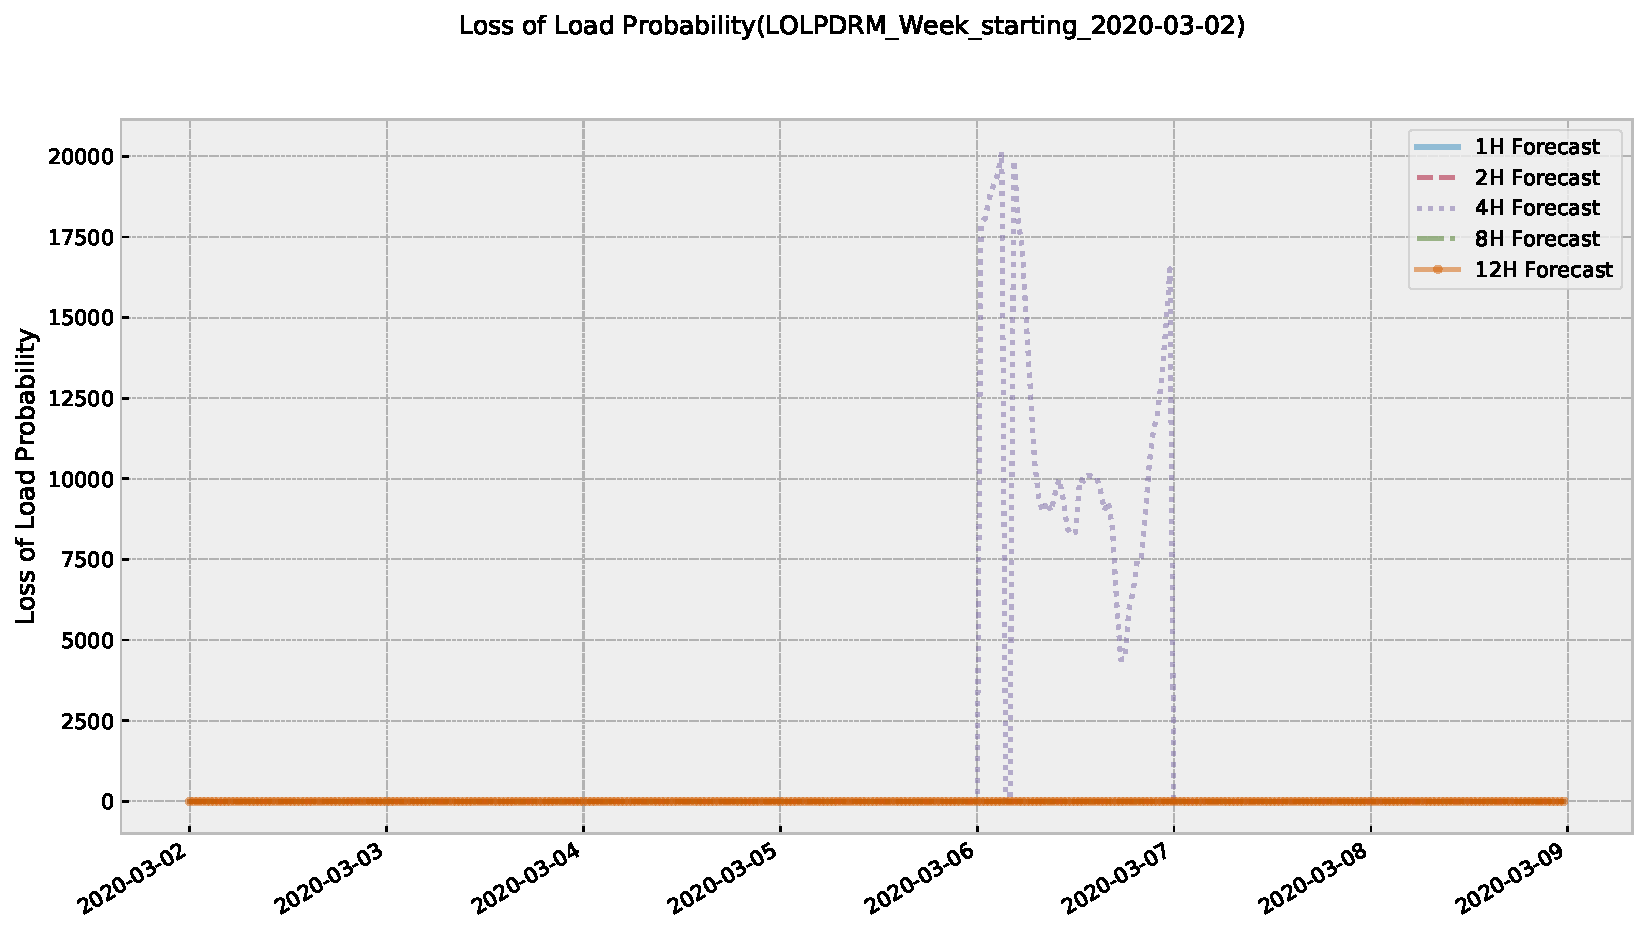
\includegraphics[width=15 cm]{Graphics/LOLPDRM_Week_starting_2020-03-02.pdf}
% \caption{}\label{}
% \end{figure}  
\begin{figure}[H]\centering
\hspace{-25pt}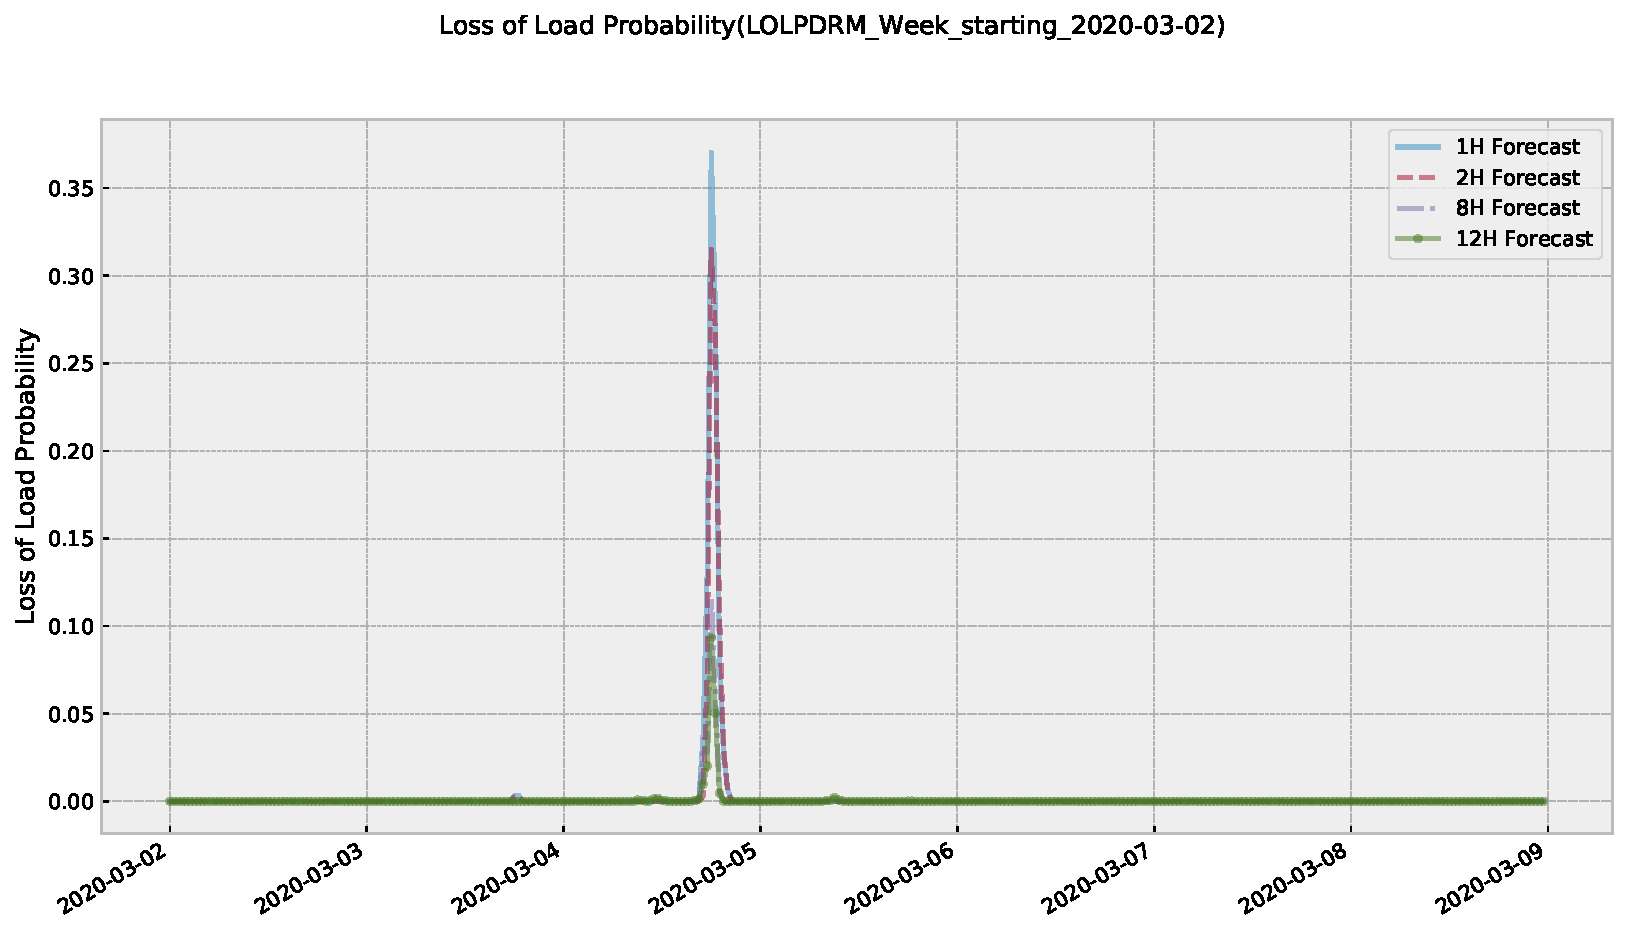
\includegraphics[width=15 cm]{Graphics/LOLPDRM_Week_starting_2020-03-02no4H.pdf}
\caption{LOLP plot for the pre-COVID-19 action week.}\label{LOLPDRM_Week_starting_2020-03-02no4H}
\end{figure}  
% \begin{figure}[H]\centering
% \hspace{-25pt}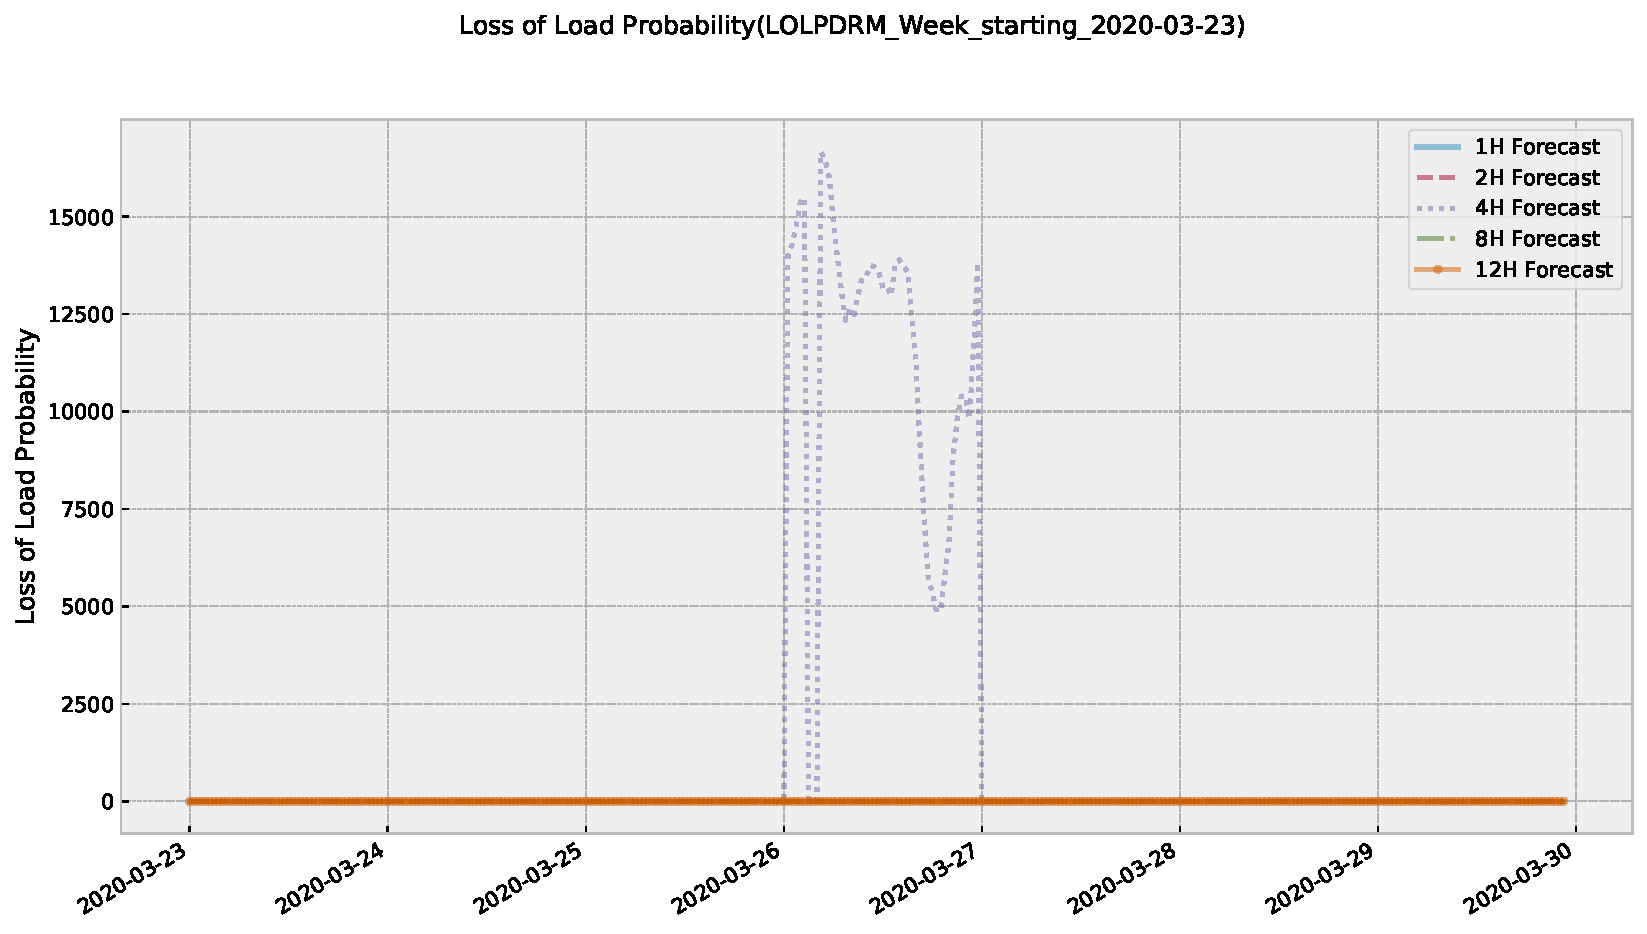
\includegraphics[width=15 cm]{Graphics/LOLPDRM_Week_starting_2020-03-23.pdf}
% \caption{}\label{}
% \end{figure}  
\begin{figure}[H]\centering
\hspace{-25pt}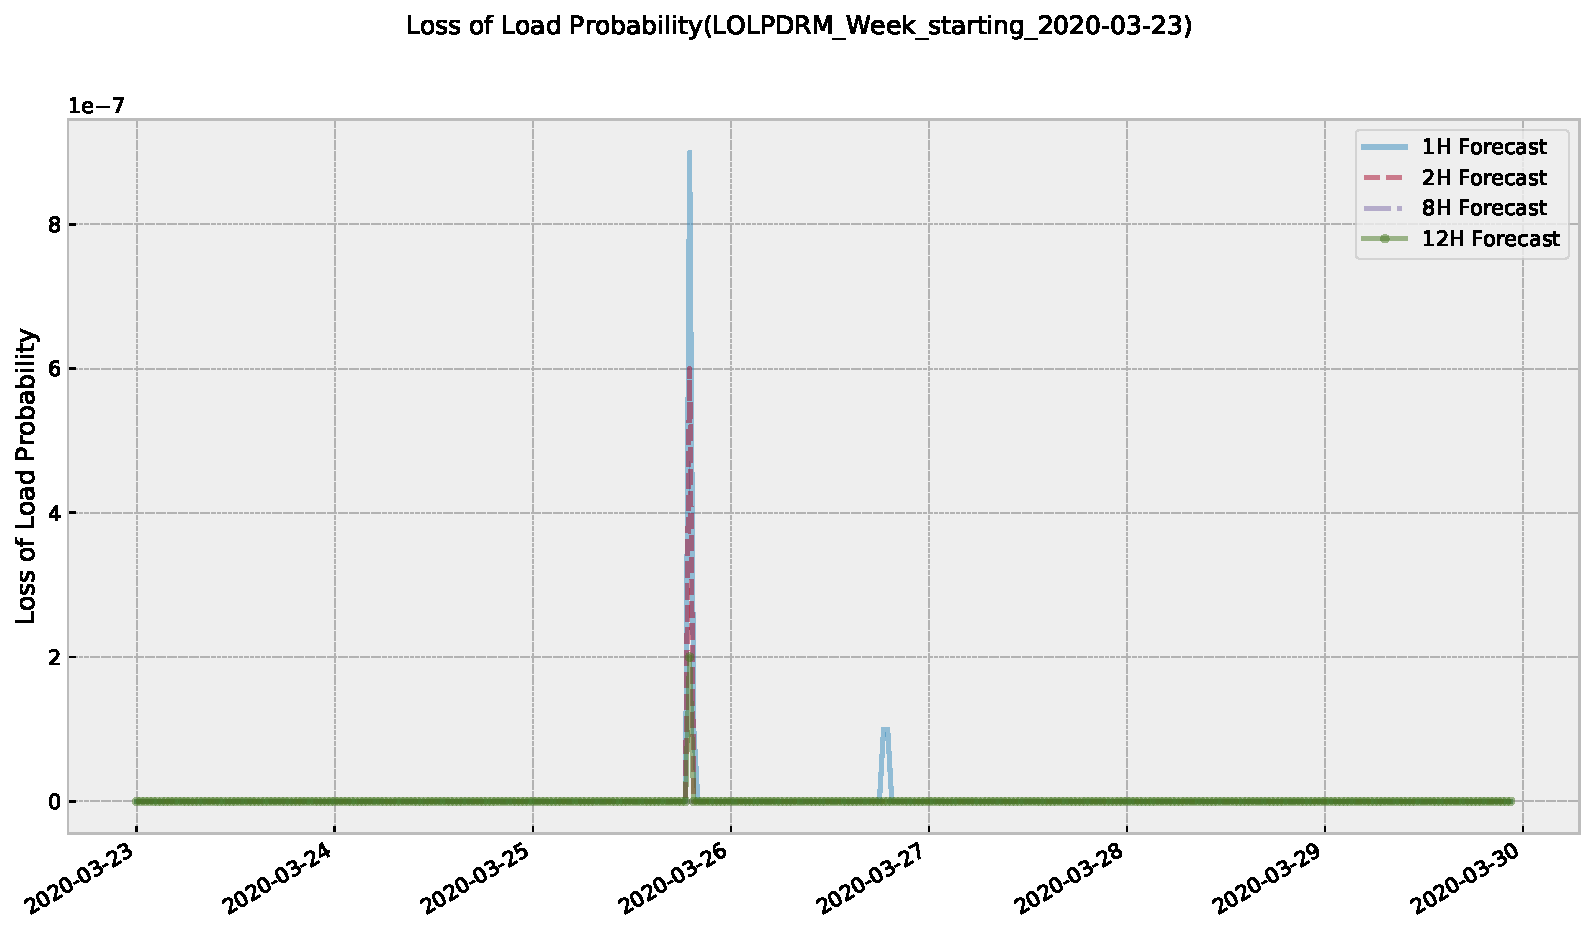
\includegraphics[width=15 cm]{Graphics/LOLPDRM_Week_starting_2020-03-23no4H.pdf}
\caption{LOLP plot for the post-COVID-19 action week.}\label{LOLPDRM_Week_starting_2020-03-23no4H}
\end{figure}  






%===============================================================
%                           REFERENCES
%===============================================================

\reftitle{References}
\externalbibliography{yes}
\bibliography{references.bib}
\bibliography{referencesmax.bib}

\end{document}



% \begin{thebibliography}{999}
% % Reference 1
% \bibitem[Author1(year)]{ref-journal}
% Author1, T. The title of the cited article. {\em Journal Abbreviation} {\bf 2008}, {\em 10}, 142--149.
% % Reference 2
% \bibitem[Author2(year)]{ref-book}
% Author2, L. The title of the cited contribution. In {\em The Book Title}; Editor1, F., Editor2, A., Eds.; Publishing House: City, Country, 2007; pp. 32--58.
% \end{thebibliography}


% To cite two works by the same author: \citeauthor{ref-journal-1a} (\citeyear{ref-journal-1a}, \citeyear{ref-journal-1b}). This produces: Whittaker (1967, 1975)
% To cite two works by the same author with specific pages: \citeauthor{ref-journal-3a} (\citeyear{ref-journal-3a}, p. 328; \citeyear{ref-journal-3b}, p.475). This produces: Wong (1999, p. 328; 2000, p. 475)

%=====================================
% References, variant B: external bibliography
%=====================================


% \section{Results}

% This section may be divided by subheadings. It should provide a concise and precise description of the experimental results, their interpretation as well as the experimental conclusions that can be drawn.
% \begin{quote}
% This section may be divided by subheadings. It should provide a concise and precise description of the experimental results, their interpretation as well as the experimental conclusions that can be drawn.
% \end{quote}

% %%%%%%%%%%%%%%%%%%%%%%%%%%%%%%%%%%%%%%%%%%
% \subsection{Subsection}
% \unskip
% \subsubsection{Subsubsection}

% Bulleted lists look like this:
% \begin{itemize}[leftmargin=*,labelsep=5.8mm]
% \item	First bullet
% \item	Second bullet
% \item	Third bullet
% \end{itemize}

% Numbered lists can be added as follows:
% \begin{enumerate}[leftmargin=*,labelsep=4.9mm]
% \item	First item 
% \item	Second item
% \item	Third item
% \end{enumerate}

% The text continues here.

% \subsection{Figures, Tables and Schemes}

% All figures and tables should be cited in the main text as Figure 1, Table 1, etc.

% \begin{figure}[H]
% \centering
% 
\includegraphics[width=2 cm]{Definitions/logo-mdpi}
% \caption{This is a figure, Schemes follow the same formatting. If there are multiple panels, they should be listed as: (\textbf{a}) Description of what is contained in the first panel. (\textbf{b}) Description of what is contained in the second panel. Figures should be placed in the main text near to the first time they are cited. A caption on a single line should be centered.}
% \end{figure}   
 
% Text

% Text

% \begin{table}[H]
% \caption{This is a table caption. Tables should be placed in the main text near to the first time they are cited.}
% \centering
% %% \tablesize{} %% You can specify the fontsize here, e.g., \tablesize{\footnotesize}. If commented out \small will be used.
% \begin{tabular}{ccc}
% \toprule
% \textbf{Title 1}	& \textbf{Title 2}	& \textbf{Title 3}\\
% \midrule
% entry 1		& data			& data\\
% entry 2		& data			& data\\
% \bottomrule
% \end{tabular}
% \end{table}

% Text

% Text

% %\begin{listing}[H]
% %\caption{Title of the listing}
% %\rule{\textwidth}{1pt}
% %\raggedright Text of the listing. In font size footnotesize, small, or normalsize. Preferred format: left aligned and single spaced. Preferred border format: top border line and bottom border line.
% %\rule{\textwidth}{1pt}
% %\end{listing}



% %%%%%%%%%%%%%%%%%%%%%%%%%%%%%%%%%%%%%%%%%%
% \section{Discussion}

% Authors should discuss the results and how they can be interpreted in perspective of previous studies and of the working hypotheses. The findings and their implications should be discussed in the broadest context possible. Future research directions may also be highlighted.

